\documentclass[jsan,article,submit,moreauthors,pdftex]{Definitions/mdpi}
%\documentclass[preprints,article,submit,pdftex,moreauthors]{Definitions/mdpi} 
%%%%%%%%%%%%%%%%%%%%%%%%%%%%%%%%%%%%%%%%%%%
\usepackage{listings}
\usepackage{xcolor}
\usepackage{caption}
%\usepackage{subcaption}
\usepackage{algorithm}
\usepackage{algpseudocode}
%\usepackage{float}
\usepackage{placeins}
\usepackage{tikz}
\usepackage{afterpage}
\usepackage{booktabs} 
\usepackage{tcolorbox}
\tcbuselibrary{listings,skins}
\usepackage{booktabs}
\usepackage{tabularx}
\usepackage{tcolorbox}
\tcbuselibrary{listings,skins}
%\usepackage{graphicx}
%\usepackage{subfig}
%\usepackage{orcidlink}
\usepackage{subcaption}
\usepackage{listings}
\usepackage{float}
\usepackage{bm} % Required for the bold math in your algorithm
%%%%%%%%%%%%%%%%%%%%%%%%%%%%%%%%%%%%%%%%%
\firstpage{1} 
\makeatletter 
\setcounter{page}{\@firstpage} 
\makeatother
\pubvolume{1}
\issuenum{1}
\articlenumber{0}
\pubyear{2026}
\copyrightyear{2026}
%\externaleditor{Firstname Lastname} % More than 1 editor, please add `` and '' before the last editor name
\datereceived{ } 
\daterevised{ } % Comment out if no revised date
\dateaccepted{ } 
\datepublished{ } 
%\datecorrected{} % For corrected papers: "Corrected: XXX" date in the original paper.
%\dateretracted{} % For retracted papers: "Retracted: XXX" date in the original paper.
%\doinum{} % Used for some special journals, like molbank
%\pdfoutput=1 % Uncommented for upload to arXiv.org
%\CorrStatement{yes}  % For updates
%\longauthorlist{yes} % For many authors that exceed the left citation part
%\IsAssociation{yes} % For association journals

%=================================================================
% Add packages and commands here. The following packages are loaded in our class file: fontenc, inputenc, calc, indentfirst, fancyhdr, graphicx, epstopdf, lastpage, ifthen, float, amsmath, amssymb, lineno, setspace, enumitem, mathpazo, booktabs, titlesec, etoolbox, tabto, xcolor, colortbl, soul, multirow, microtype, tikz, totcount, changepage, attrib, upgreek, array, tabularx, pbox, ragged2e, tocloft, marginnote, marginfix, enotez, amsthm, natbib, hyperref, cleveref, scrextend, url, geometry, newfloat, caption, draftwatermark, seqsplit
% cleveref: load \crefname definitions after \begin{document}

%=================================================================
% Please use the following mathematics environments: Theorem, Lemma, Corollary, Proposition, Characterization, Property, Problem, Example, ExamplesandDefinitions, Hypothesis, Remark, Definition, Notation, Assumption
%% For proofs, please use the proof environment (the amsthm package is loaded by the MDPI class).

%=================================================================
% Full title of the paper (Capitalized)
\Title{STGen: A Lightweight Sensor Testbed for Scenario-Based IoT Protocol Evaluation}


% Authors, for the paper (add full first names)

% Authors, for the paper (add full first names)
\Author{Hasan MA Islam $^{1,*}$\orcidA, Md MR Maharaz $^{1}$\orcidB, M Georgiades $^{2}$\orcidC, SMN Shahriar $^{1}$\orcidD, P Akibuzzaman $^{1}$\orcidE, NJ Aurna$^{1}$\orcidF and Riadul Islam $^{3}$\orcidG}

% \longauthorlist{yes}

% MDPI internal command: Authors, for metadata in PDF
\AuthorNames{Hasan MA Islam, Md MR Maharaz, Michael Georgiades, SMN Shahriar, P Akibuzzaman, NJ Aurna and Riadul Islam}

% Affiliations / Addresses (Add [1] after \address if there is only one affiliation.)
\address{%
$^{1}$ \quad Dept. of Computer Science and Engineering, East West University; hasan.mahmood@ewubd.edu\\
$^{2}$ \quad Dept. of Computer Science, Neapolis University of Pafos; m.georgiades@nup.ac.cy\\
$^{3}$ \quad University of Maryland, Baltimore County; riaduli@umbc.edu}


% Contact information of the corresponding author
\corres{Correspondence: hasan.mahmood@ewubd.edu}

% Current address and/or shared authorship
%\firstnote{Current address: Affiliation.}  
% Current address should not be the same as any items in the Affiliation section.

%\secondnote{These authors contributed equally to this work.}
% The commands \thirdnote{} till \eighthnote{} are available for further notes.

%\simplesumm{} % Simple summary

%\conference{} % An extended version of a conference paper

% % Abstract (Do not insert blank lines, i.e. \\) 
% \abstract{This paper introduces the Sensor Traffic Generator (STGen), a lightweight, pure-software testbed for evaluating {IoT} application-layer and transport-layer protocols at scale. Operating above OSI Layer~4, STGen does not model PHY or MAC behavior (RF interference, CSMA/CA collision avoidance, duty cycling), which keeps the evaluation on the protocol logic that researchers actually write. Thousands of virtual sensor nodes  run in software and generate stochastic sensor streams governed by physical models. Its sensor models are calibrated against 1,826,223 real-world readings from the Intel Berkeley Research Laboratory; for temperature the synthetic stream matches the 37-day field measurements of 54 Mica2Dot motes with a Kolmogorov-Smirnov $D$ of 0.071 and a Jensen-Shannon Divergence of 0.018, establishing that the generated traffic reproduces the statistical structure of real sensor data rather than merely plausible values. A modular three-tier architecture separates experiments into {IoT} Protocols ($N$), Scenarios ($M$), and Network ($L$) tiers, reducing cross-domain configuration effort from a combinatorial ($N \times M \times L$) to a linear ($N+M+L$) problem, and any conforming protocol is integrated by overriding a four-method abstract interface. In our experiments, STGen instantiates 6{,}000 concurrently emulated nodes, each an independent operating-system process, on a commodity workstation in 1.02\,s using 0.62\,GB of memory (99\,KB per node), more than two orders of magnitude less memory per emulated node than the container and VM-based testbeds. Furthermore, it exposes deployment-relevant behavior such as MQTT reconnect storms under wide-area jitter that purely emulated environments do not reveal.}

\abstract{This paper introduces the Sensor Traffic Generator (STGen), a lightweight, pure-software testbed for evaluating IoT application-layer and transport-layer protocols at scale. STGen operates above OSI Layer 4 and therefore does not model PHY- or MAC-layer behavior such as RF interference, CSMA/CA collision avoidance, or duty cycling. Instead, it provides a controlled baseline for studying the protocol logic implemented by researchers, with the link layer treated as ideal or uniformly degraded. Thousands of virtual sensor nodes run in software and generate stochastic sensor streams governed by physically grounded models. These models are calibrated against 1,826,223 real-world readings from the Intel Berkeley Research Laboratory; for temperature, the synthetic stream matches the 37-day measurements of 54 Mica2Dot motes with a Kolmogorov-Smirnov D of 0.071 and a Jensen-Shannon Divergence of 0.018, showing that STGen reproduces the statistical structure of real sensor data rather than only plausible values. By inverting these calibrated models, STGen also synthesises labelled false-data-injection anomalies, separable from normal traffic at a receiver-operating-characteristic AUC of 0.955 for stealthy drift and 1.0 for hard physical-range violations. STGen uses a modular three-tier architecture that separates experiments into IoT Protocols (N), Scenarios (M), and Network (L) tiers, reducing configuration effort from a combinatorial N x M x L problem to a linear N + M + L workflow. New protocols can be integrated by overriding a four-method abstract interface, making the framework protocol-agnostic and extensible. In our experiments, STGen instantiates 6,000 concurrently emulated sensor nodes, each represented as an independent operating-system process, on a commodity workstation in 1.02 s using 0.62 GB of memory, corresponding to approximately 99 KB per node for the lightweight process-based node model. This is more than two orders of magnitude lower than the per-node memory cost of container- and VM-based testbeds. Beyond scalability, STGen also exposes deployment-relevant behavior that controlled emulation alone may hide: under live wide-area jitter, MQTT and CoAP exhibit different loss and latency patterns from those observed under uniformly degraded NetEm conditions, including MQTT reconnect storms. These results show that STGen provides a scalable, reproducible, and protocol-agnostic bridge between lightweight protocol emulation and practical deployment-oriented IoT protocol evaluation.}
% Keywords
\keyword{IoT testbed; protocol evaluation; synthetic sensor data; wireless sensor networks; network emulation; MQTT; CoAP; scalability}


%%%%%%%%%%%%%%%%%%%%%%%%%%%%%%%%%%%%%%%%%%
% ORCID definitions
\newcommand{\orcidauthorA}{0009-0005-7028-7902} % Hasan MA Islam
\newcommand{\orcidauthorB}{0009-0006-4513-6552} % Mahamudur Rahman Maharaz
\newcommand{\orcidauthorC}{0009-0006-7414-6434} % S. M. Nafis Shahriar
\newcommand{\orcidauthorD}{0009-0004-4119-2333} % Pulok Akibuzzaman
\newcommand{\orcidauthorE}{0009-0006-9867-7117} % Subrata Nath
\newcommand{\orcidauthorF}{0009-0005-4056-9757} % Mahdin Islam Ohi
\newcommand{\orcidauthorG}{0000-0002-5930-8814} % Michael Georgiades
\newcommand{\orcidauthorH}{0000-0002-4649-3467} % Riadul Islam

\begin{document}
\setlength{\headheight}{20.0pt}
\nolinenumbers


%%%%%%%%%%%%%%%%%%%%%%%%%%%%%%%%%%%%%%%%%%

\section{Introduction}
\label{sec:introduction}
Wireless Sensor Networks (WSNs) are distributed sensor networks that collect data from their surroundings and broadcast within range \cite{YICK20082292, matin2012overview}. These are similar to ad-hoc networks \cite{ramanathan2002brief} in that they rely on wireless connectivity and spontaneous network formation to transport sensor data. A typical sensor node consists of a communication module, a processing unit, multiple sensor interfaces, and a power source, usually a battery or an embedded energy source \cite{5522465}. The energy limitation, along with the computational constraints of the sensor nodes, requires efficient protocol design and evaluation to improve efficiency \cite{saginbekov2016testing}. As network infrastructure simultaneously spans severely constrained low-power links (e.g., LoRaWAN at 250 \,bit/s) and high-throughput backhauls (e.g., 5G NR at multi-Gbps), evaluation frameworks must characterize the application-layer and transport-layer protocol behavior throughout the entire link-capacity spectrum~\cite{fi15110348}.

\begin{table}[ht]
\centering
\footnotesize
\caption{Common network simulators used for WSN evaluation}
\renewcommand{\arraystretch}{1.3}
\begin{tabularx}{\columnwidth}{l l X l l}
\hline
\textbf{Sim} & \textbf{Lang} & \textbf{Focus} & \textbf{Curve} & \textbf{Scale} \\
\hline
ns-3~\cite{riley2010ns} & C++ & Packet-level net sim, PHY/MAC models. & High & $10^4$+ \\
OMNeT++~\cite{varga2008overview}& C++ & Modular protocol sim; component modeling. & V. High & \ 3000+\footnote{https://www.spec.org/cpu2006/Docs/471.omnetpp.html} \\
Cooja  ~\cite{velinov2016running} & Java & OS-level emulation (Contiki), WSNs. & Mod. & $<100$ \\
\hline
\end{tabularx}

\label{tab:simulator-limits}
\end{table}
%%%%%%%%%%%%%%%%%%%%%%%%%%%%%%%%%%%%%%%%%%%%
% \begin{table*}[ht]
% \centering
% \footnotesize
% \renewcommand{\arraystretch}{1.3}
% \newcolumntype{L}{>{\raggedright\arraybackslash}X} 

% \caption{Comparison of IoT Protocol Evaluation Testbeds and Frameworks. (N/R = Not Reported, Mod. = Moderate)}
% \label{tab:testbed-comparison}

% \begin{tabularx}{\textwidth}{l l L L l l l}
% \hline
% \textbf{System} & \textbf{Type} & \textbf{Architecture / Scale} &
% \textbf{Protocols} & \textbf{Boot Time} &
% \textbf{Mem} & \textbf{Net Emul.} \\
% \hline

% % --- SECTION 1 ---
% \multicolumn{7}{l}{\textit{\textbf{Physical Testbeds}}} \\
% FIT IoT-LAB \cite{adjih2015fit} & Phy & Physical nodes (2700+ devices) & Hardware (any) & N/A & N/R & Ext. Tools \\
% SmartSantander \cite{sanchez2014smartsantander} & Phy & City-wide heterogeneous & Various & N/A & N/R & No \\

% \hline
% % --- SECTION 2 ---
% \multicolumn{7}{l}{\textit{\textbf{VM-Based \& Hybrid Testbeds}}} \\
% Gotham \cite{saez2023gotham} & Hybrid & Docker + QEMU ($\sim$10 GB) & MQTT, CoAP & $>$20 min & $\sim$10 GB & Limited \\
% GothX \cite{poisson2024gothx} & Hybrid & VM + Docker ($\sim$20 GB RAM) & MQTT, Kafka & $\sim 26$ min & 20 GB & Limited \\
% IOTier \cite{nikolaidis2021iotier} & Virt & Cluster-based & Agnostic & $>$5 min & High & Yes \\

% \hline
% % --- SECTION 3 ---
% \multicolumn{7}{l}{\textit{\textbf{Application Frameworks \& Simulators}}} \\
% IoT-Flock \cite{ghazanfar2020iot} & Frmwk & App-level (Host dependent) & MQTT, CoAP & Mod. & $\sim$400 MB & No \\
% Patr{IoT} \cite{bures2021patriot} & Frmwk & JUnit-based (CI/CD) & Code-defined & N/R & High & No \\
% IoTSim-Edge \cite{jha2020iotsim} & Sim & Edge/Cloud Modeling & Stream/MapRed & Mod. & N/R & Abstract \\
% TOSSIM \cite{10.1145/958491.958506} & Sim & Discrete Event & TinyOS Only & Fast & Low & Built-in \\
% SENS \cite{sundresh2004sens} & Sim & Generic Framework & Generic & Mod. & N/R & No \\

% \hline
% % --- YOUR WORK ---
% % \textbf{STGen (This Work)} & \textbf{Proc} & \textbf{Process-based (6000+ nodes)} & \textbf{Pluggable} & \textbf{$\sim$1.02 s} & \textbf{0.62 GB} & \textbf{Yes} \\
% \textbf{STGen (This Work)} & \textbf{Proc} & \textbf{Process-based (6000+ nodes)} & \textbf{Pluggable} & \textbf{0.32--1.02 s}$^\dagger$ & \textbf{0.62 GB} & \textbf{Yes} \\
% \hline
% \end{tabularx}
% \multicolumn{7}{l}{\footnotesize{$^\dagger$Startup scales linearly with node count: 0.32\,s at 100 nodes, 0.44\,s at 1{,}000 nodes, 1.02\,s at 6{,}000 nodes ($R^2=0.9995$). See Table~\ref{tab:scalability}.}} \\
% \end{table*}


%%%%%%%%%%%%%%%%%%%%%%%%%%%%%%%%%%%%%%%%%%%%%%%%%%%%

Protocol researchers and network engineers often use traffic generation tools to benchmark network performance and troubleshoot problems \cite{swann2021tools}. Although many frameworks and tools \cite{saez2023gotham, poisson2024gothx, ghazanfar2020iot, bures2021patriot,li2024iotgemini,sundresh2004sens} have been proposed by research communities and software industries, most of them lack support for lightweight and easily configurable traffic generation capabilities, as well as extensibility for Internet of Things (IoT) specific application-layer protocols, particularly in controlled environments such as WSNs. 

Several widely used network simulators have been proposed for evaluating WSNs, each offering different trade-offs in scalability, modeling fidelity, and ease of use, as summarized in Table~\ref{tab:simulator-limits}. Although network simulators give users control over the entire network stack, they create challenges in testing application-layer protocols. For example, OMNeT++~\cite{varga2008overview} requires advanced C++ proficiency, presenting a substantial barrier to entry for researchers. ns-3~\cite{riley2010ns} requires complex setup and configuration through Python or C++. Cooja (Contiki)~\cite{velinov2016running} provides a real operating system-based simulation, but suffers from limited scalability and a Java-based GUI. Although these tools are strong for network-layer research, developing application-layer protocols can take weeks or even months. STGen does not replace ns-3, OMNeT++, or Cooja: those reproduce PHY- and MAC-layer dynamics. In contrast, this work targets the complementary problem, the early-stage evaluation of application- and transport-layer protocols at thousands-of-nodes scale, where PHY/MAC fidelity is not the variable under study, and scalability and real protocol-stack behavior are.

In order to facilitate the analysis of a protocol evaluation, this article proposes STGen, a lightweight, protocol-agnostic, scenario-based testbed designed to emulate large-scale IoT-based wireless sensor network (WSN) environments. STGen instantiates thousands of virtual sensor nodes that produce a high volume of sensor traffic. It can be used for assessing protocol performance in traditional IoT networks where bandwidth is limited, but also for evaluating the scalability, CPU performance, and end-to-end latency in networks representative of modern high-speed networks.

The STGen Core is able to handle a large number of virtual sensor nodes with low memory overhead, allowing large-scale application- and transport-layer experiments to be conducted on a single machine. Moreover, STGen's scenario-based architecture makes use of extensible JSON scenarios that allow for the definition of domain-specific scenarios, like smart healthcare and smart home scenarios. This way, researchers can closely recreate real-world conditions and test protocols across a variety of application scenarios. Overall, the design enables the easy integration of simulated IoT environments and real-world application clients, which enables scalable, repeatable and practical protocol research.

% \begin{sloppypar} To enable extensive and scalable protocol evaluation, this article introduces STGen, a lightweight, protocol-agnostic, scenario-based testbed designed to emulate large-scale IoT-based wireless sensor network (WSN) environments. STGen supports the instantiation of thousands of virtual sensor nodes that generate high-volume sensor traffic. This makes it suitable not only for evaluating protocol performance in traditional {IoT} settings with limited bandwidth, but also for assessing scalability, CPU efficiency, and end-to-end latency under conditions representative of modern high-speed networks. \end{sloppypar} 



% The STGen Core efficiently manages a large number of virtual sensor nodes while maintaining low memory overhead, enabling realistic large-scale experimentation on a single machine. In addition, STGen’s scenario-based architecture leverages extensible JSON files to define domain-specific scenarios, such as smart healthcare and smart home environments. This approach allows researchers to closely mimic real-world conditions and evaluate protocols in diverse application contexts. In general, the design facilitates seamless integration between emulated {IoT} environments and real-world client applications, thus supporting scalable, reproducible and practical protocol research.

% To validate the capabilities of STGen, we implemented a custom application-layer protocol built on top of UDP \cite{postel1980rfc768}, following a publish/subscribe communication paradigm \cite{fotiou2012illustrating}. Protocol, scenario, and network configurations can be crafted to reflect realistic deployment environments, enabling the transmission of synthetic data to a designated sink node, the STGen Core in our architecture. The STGen Core handles resource-intensive tasks such as maintaining the client state table and delivering data to clients immediately upon subscription. Our evaluation focuses explicitly on the end-to-end communication path between external clients and the STGen Core using this custom protocol. This includes measuring performance metrics, notably latency, packet loss, and memory and CPU utilization under varying load levels. Throughout the communication process, network traffic, including sensor data, is logged for subsequent analysis. These logs are utilized in conjunction with a robust data visualization stack (ELK) \cite{sachdeva2017practical} to assess system performance and obtain deeper analytical insights.

To evaluate STGen, we measure end-to-end latency, packet loss, and host resource scaling (CPU and memory) under varying load levels using a custom UDP-based publish-subscribe protocol \cite{postel1980rfc768, fotiou2012illustrating}. The STGen Core acts as the designated sink node, servicing concurrent subscriptions and forwarding captured network traffic to an ELK stack \cite{sachdeva2017practical} for real-time latency and jitter extraction.

STGen enables researchers and developers to prototype device integration and evaluate the behavior of {IoT} application services such as real-time monitoring, traffic shaping and edge-level data analytics.

We frame the work around four questions. \textbf{(RQ1)} Can physically grounded synthetic sensor streams reproduce the statistical structure (marginal, temporal, and cross-modality) of real deployment data? \textbf{(RQ2)} Can a process-based architecture scale beyond VM- and container-based approaches on commodity hardware while keeping per-node cost low? \textbf{(RQ3)} Can such a testbed expose protocol behavior that packet-level simulation hides? \textbf{(RQ4)} Can the same physically-validated models generate labelled application-layer anomalies that are statistically separable from normal traffic? 

The key contributions of this work are as follows.
\vspace{.1cm}

\begin{enumerate}
    \item A physically validated synthetic sensor generator. Temperature, humidity, light, and voltage streams are produced by hardware-grounded models (Ornstein-Uhlenbeck thermal drift, PIR refractory logic, MEMS noise floors) and validated against 1,826,223 real readings from the Intel Berkeley deployment, matching the marginal distribution (temperature Kolmogorov-Smirnov $D=0.071$), the temporal structure (autocorrelation within 0.035 of the measured curve at every tested lag), and the cross-modality coupling (temperature-humidity Pearson $r=-0.403$ against the measured $-0.426$).
    \item A three-tier protocol/scenario/network decomposition that reduces experiment-specification effort from a multiplicative $N \times M \times L$ to an additive $N+M+L$.
    \item A process-based emulation model that instantiates 6{,}000 independent sensor-node processes on one 16\,GB workstation at a marginal 99\,KB per node, where each process holds a live transport stack and exposes per-message latency, loss, and session state rather than an aggregate count.
    \item Evidence that the protocol behavior observed under emulated (NetEm) congestion does not carry over to a live deployment: across a three-site Tailscale/WireGuard overlay in Dhaka, the MQTT/CoAP loss ordering \emph{inverts} relative to the emulated benchmark, because steady-state uniform loss and bursty wide-area loss stress the two transports differently. A distributed deployment model in which software-defined nodes run across heterogeneous hosts and report to a central sink supports this measurement.
    \item A reproducible evaluation workflow. STGen includes named scripts for regenerating the reported tables and figures, statistical checks for protocol-latency comparisons, and a dual-archiving mechanism using local files and MongoDB to preserve sensor streams during long-running experiments.
    \item An integrated adversarial engine that produces reproducible, labelled false-data-injection (FDI) datasets by perturbing STGen's statistically validated sensor models. This feature generates configurable attack scenarios with complete ground-truth labels, enabling systematic benchmarking of protocol resilience and anomaly-detection methods.
   

\end{enumerate}

The remainder of the article is organized as follows: Section~\ref{sec:related_work} reviews existing {IoT} testbeds and identifies the gaps in scalability and architectural flexibility that STGen addresses. The core components and system architecture, including the physically-validated sensor profiles and the three-tier configuration model, are detailed in Section~\ref{sec:system_architecture}. Section~\ref{sec:setup} describes the simulation metrics, the network emulation profiles, and the hardware environment utilized for the benchmarking.  The evaluation methodology of the STGen framework is detailed in Section~\ref{sec:eval_stgen}. The experimental findings and discussion are provided in Section~\ref{sec:Experiment}. Section~\ref{sec:protocol-agnosticism} discusses the protocol-agnostic nature of the framework and the integration workflow for custom protocols. Section~\ref{sec:threats} states the limitations and threats to validity. Potential future work is described in Section~\ref{sec:future-work}. Moreover,  Section~\ref{sec:reproducibility} documents reproducibility and artifact availability. Finally, Section~\ref{sec:conclusion} concludes the article.

\section{State of the Art}
\label{sec:related_work}

In recent years, several experimental testbeds have been developed to support large-scale {IoT} environments for the experimentation of {IoT} protocols and their applications. For example, FIT IoT-LAB \cite{adjih2015fit} and SmartSantander \cite{sanchez2014smartsantander} have advanced the field by providing researchers with extensive sensor networks. However, these testbeds often come with limitations in node accessibility and complex configurations. For instance, the main limitations of SmartSantander are its battery life and limited user reprogramming options, while FIT IoT-LAB focuses on providing access to bare metal but requires careful management of heterogeneous nodes and experimental setup.

SENS~\cite{sundresh2004sens} is a modular simulator for wireless sensor networks that integrates sensor, environment, and network components. It enables realistic modeling of physical environments using tile-based propagation and supports application portability by allowing the same source code to run on simulated and real nodes. However, SENS is an older framework focused on component-based WSNs and provides limited support for evaluating modern {IoT} application-layer protocols.

TOSSIM \cite{10.1145/958491.958506} is a discrete event simulator designed to be used with the TinyOS operating system. It is high-fidelity in the sense that it just in time builds TinyOS component graphs into the simulation infrastructure, allowing network behavior to be modeled at the bit level.  However, TOSSIM is closely linked to the TinyOS-nesC environment and is therefore not suitable for analyzing general-purpose {IoT} application protocols, such as MQTT or CoAP, running on a generic embedded C or Linux platform. Besides, its implementation model fails to consider CPU time sharing or preemption, and performance is reduced considerably when dealing with network-intensive workloads.

Several frameworks have attempted to bridge the gap between simulation and emulation. IoTSim-Edge~\cite{jha2020iotsim} focuses on modeling edge computing behaviors, whereas IOTier~\cite{nikolaidis2021iotier} offers a fully virtualized testbed environment. However, recent benchmarking by Bendaouch et al.~\cite{bendaouch2025benchmarking} demonstrates that multi-tier (Edge-Fog-Cloud) simulations suffer from substantial computational overhead, largely stemming from heavy virtualization dependencies.

%%%%%%%%%%%%%%%%%%%%%%%%%%%%%%%%%%%%%%%%%%
\begin{table*}[ht]
\centering
\footnotesize
\renewcommand{\arraystretch}{1.3}


\caption{Comparison of IoT Protocol Evaluation Testbeds and Frameworks. (N/R = Not Reported, Mod. = Moderate)}
\label{tab:testbed-comparison}

\begin{tabularx}{\textwidth}{l l L L l l l}
\hline
\textbf{System} & \textbf{Type} & \textbf{Architecture / Scale} &
\textbf{Protocols} & \textbf{Boot Time} &
\textbf{Mem} & \textbf{Net Emul.} \\
\hline

% --- SECTION 1 ---
\multicolumn{7}{l}{\textit{\textbf{Physical Testbeds}}} \\
FIT IoT-LAB \cite{adjih2015fit} & Phy & Physical nodes (2700+ devices) & Hardware (any) & N/A & N/R & Ext. Tools \\
SmartSantander \cite{sanchez2014smartsantander} & Phy & City-wide heterogeneous & Various & N/A & N/R & No \\

\hline
% --- SECTION 2 ---
\multicolumn{7}{l}{\textit{\textbf{VM-Based \& Hybrid Testbeds}}} \\
Gotham \cite{saez2023gotham} & Hybrid & Docker + QEMU ($\sim$10 GB) & MQTT, CoAP & $>$20 min & $\sim$10 GB & Limited \\
GothX \cite{poisson2024gothx} & Hybrid & VM + Docker ($\sim$20 GB RAM) & MQTT, Kafka & $\sim 26$ min & 20 GB & Limited \\
IOTier \cite{nikolaidis2021iotier} & Virt & Cluster-based & Agnostic & $>$5 min & High & Yes \\

\hline
% --- SECTION 3 ---
\multicolumn{7}{l}{\textit{\textbf{Application Frameworks \& Simulators}}} \\
IoT-Flock \cite{ghazanfar2020iot} & Frmwk & App-level (Host dependent) & MQTT, CoAP & Mod. & $\sim$400 MB & No \\
Patr{IoT} \cite{bures2021patriot} & Frmwk & JUnit-based (CI/CD) & Code-defined & N/R & High & No \\
IoTSim-Edge \cite{jha2020iotsim} & Sim & Edge/Cloud Modeling & Stream/MapRed & Mod. & N/R & Abstract \\
TOSSIM \cite{10.1145/958491.958506} & Sim & Discrete Event & TinyOS Only & Fast & Low & Built-in \\
SENS \cite{sundresh2004sens} & Sim & Generic Framework & Generic & Mod. & N/R & No \\

\hline
% --- YOUR WORK ---
\textbf{STGen (This Work)} & \textbf{Proc} & \textbf{Process-based (6000+ nodes)} & \textbf{Pluggable + FDI}$^{\ddagger}$ & \textbf{0.32--1.02 s}$^\dagger$ & \textbf{0.62 GB} & \textbf{Yes} \\
\hline
\end{tabularx}
\vspace{2pt}
\raggedright \footnotesize{$^\dagger$Startup scales linearly with node count: 0.32\,s at 100 nodes, 0.44\,s at 1{,}000 nodes, 1.02\,s at 6{,}000 nodes ($R^2=0.9995$). See Table~\ref{tab:scalability}.\\
$^{\ddagger}$STGen additionally generates labelled false-data-injection (FDI) anomalies as departures from its physically-validated baseline (Section~\ref{sec:adversarial}).}
\end{table*}
Gotham \cite{saez2023gotham} and GothX \cite{poisson2024gothx} are tools for creating {IoT} datasets with both legitimate and malicious traffic. Gotham supports protocols such as MQTT and CoAP. GothX adds Kafka and SINETStream for better {IoT} traffic generation. These tools allow testing across different communication protocols and automate scenario execution. GothX offers greater flexibility with customizable topologies and automatic dataset labeling. They run each emulated IoT device as a Docker container and each network router as a QEMU virtual machine, which costs about 37\,MB per device and 470\,MB per router VM \cite{poisson2024gothx}. On a resource-constrained workstation, this limits the testbed at a few hundred nodes before memory is exhausted, and the shared virtualization layer adds resource contention between co-located guests.

the use of heavy virtualization technologies can incur significant resource overhead. This leads to long boot times and higher memory usage, constraining the maximum node density that can be run on a single machine. These tools generate network-level attack traffic; STGen instead injects application-layer false-data anomalies defined as departures from a physically-validated sensor baseline (Section~\ref{sec:adversarial}), and labels every record, which is a different point in the design space rather than a replacement.

The Patr{IoT} \cite{bures2021patriot} has been developed to offer a flexible {IoT} system testbed. This testbed scales from a physical setup to a simulated environment and supports mixed configurations. The framework is built on JUnit 5, which has been extended to support interoperability and integration testing. However, Patr{IoT} requires users to explicitly manage complex event synchronization within the test code, which increases the development effort and complexity when simulating asynchronous {IoT} network conditions.

IoT-Flock \cite{ghazanfar2020iot} is an open-source framework that creates {IoT} traffic to help develop security solutions for smart homes by mimicking real-world {IoT} devices. It works with two {IoT} application-layer protocols such as MQTT and CoAP. However, its native execution is currently non-functional, mandating a VM deployment, which introduces substantial hypervisor overhead. Furthermore, it does not publish resource-utilization metrics, making it difficult to assess its viability for large-scale benchmarking where resource constraints are critical.

{IoTGemini}~\cite{li2024iotgemini} generates synthetic {IoT} traffic that models device functions and network behaviors using Packet Sequence GAN (PS-GAN). The framework focuses on statistical traffic modeling rather than stateful protocol execution. Consequently, it is unable to confirm the functional integrity of the application-layer protocols, including the integrity of message delivery.

Table~\ref{tab:testbed-comparison} compares STGen against representative physical testbeds, VM-based and hybrid platforms, simulators, and application-level frameworks. The comparison reveals a consistent gap: existing platforms either provide high-fidelity physical or packet-level modelling with limited ease of application-layer protocol experimentation, or support IoT traffic generation at the cost of heavy virtualization overhead, limited scalability, weak network-emulation support, or restricted protocol extensibility. These limitations motivate the need for a lightweight, scalable, and protocol-agnostic architecture that can support repeatable application- and transport-layer IoT protocol evaluation on commodity hardware.

\begin{figure*}[ht]
  \centering
  \includegraphics[width=.95\textwidth]{images/base_diagram.jpg}
  \caption{
  Overview of the STGen Distributed {IoT} Evaluation Architecture. The framework bridges the Distributed Sensor World with analytical {IoT} Applications via the central Protocol-Agnostic STGen Core, facilitating comprehensive protocol evaluation under realistic network conditions. }
  \label{stgen-eco-overview}
\end{figure*}

% \begin{figure*}[htbp]
%   \centering
%   \includegraphics[width=\textwidth]{images/STGen_System_architecture.jpg}
%   \caption{ 
%   Workflow diagram of STGen testbed.
%  }
%   \label{fig:sys_archi_2}
% \end{figure*}



%%%%%%%%%%%%%%%%%%%%%%%%%%%%%%%%%%%%%%%%%%
%%%%%%%%%%%%%%%%%%%%%%%%%%%%%%%%%%%%%%%%%%
\section{System Architecture of STGen}

\label{sec:system_architecture}

STGen provides a flexible and extensible platform for simulating {IoT} environments and testing communication protocols. Its architecture is designed to support diverse scenarios while ensuring scalability and modularity.


\subsection{Architectural Overview}
\label{sec:sub_architectural_overview}
% The high-level architecture of STGen is presented in Fig.~\ref{stgen-eco-overview}. The STGen core acts as the middleware between the distributed sensor world and the client. In the distributed model, multiple STGen core instances can run concurrently, where each core coordinates numerous emulated sensors and client nodes.  Fig.~\ref{fig:sys_archi_2} shows the STGen workflow sequence, demonstrating the flow of configuration, orchestration, and observation. This structural decoupling allows for easy testing of various protocols in different scenarios such as smart homes, smart agriculture, or industrial {IoT} (IIoT) \cite{stojkoska2017review, sfar2018roadmap} without changing the core itself. During a run, the observability layer collects logs and performance metrics so that protocol behavior can be compared across workloads and traffic patterns.

The high-level architecture of STGen is presented in Fig.~\ref{stgen-eco-overview}. The STGen core acts as the middleware between the distributed sensor world and the client. In the distributed model, multiple STGen core instances can run concurrently, where each core coordinates numerous emulated sensors and client nodes. This structural decoupling allows for easy testing of various protocols in different scenarios such as smart homes, smart agriculture, or industrial {IoT} (IIoT) \cite{stojkoska2017review, sfar2018roadmap} without changing the core itself. During a run, the observability layer collects logs and performance metrics so that protocol behavior can be compared across workloads and traffic patterns.



\subsection{Core Components}
\label{core-components}

The core components of STGen tesbed are described below:

\begin{table*}[ht]
\centering
\caption{Summary of Mathematical Variables and Parameters used in STGen Sensor Profiles}
\label{tab:nomenclature}
\begin{tabularx}{\textwidth}{@{}lllX@{}}
\toprule
\textbf{Category} & \textbf{Symbol} & \textbf{Unit/Type} & \textbf{Description} \\ \midrule
\textbf{Thermal Dynamics} \cite{uhlenbeck1930} & $T_t$ & $^\circ\text{C}$ / Float & Temperature value at time $t$  \\
 & $\theta$ & $\text{s}^{-1}$ & Thermal relaxation rate (resistance to change)  \\
 & $\mu$ & $^\circ\text{C}$ & Long-term mean or ambient temperature \\
 & $dW_t$ & Brownian & Wiener process (Gaussian white noise)  \\ \midrule
\textbf{Hardware Constraints} \cite{hcsr501, mpu6050}  & $T_{\text{dwell}}$ & s & Sensor high-state duration after activation \\
 & $T_{\text{blocking}}$ & s & Refractory period where sensor is unresponsive  \\
 & $\sigma_{\text{noise}}$ & RMS & Calculated noise floor for vibration sensing  \\
 & NSD & $\mu g/\sqrt{\text{Hz}}$ & Noise Spectral Density from device datasheet  \\
 & $BW$ & Hz & Sensor bandwidth  \\ \midrule
\textbf{Mobility \& Kinematics} \cite{bettstetter2001, snyder1987map}  & $v_{\max}$ & m/s & Maximum allowable user or asset speed \\
 & $\Delta t$ & s & Time interval between generation steps \\
 & $\Delta_{\text{deg}}$ & Degrees & Geodesic distance change in coordinates  \\ \midrule
\textbf{Traffic \& Control} \cite{6662948} & $k$ & Shape ($k < 1$) & Weibull parameter controlling burstiness  \\
 & $\lambda$ & Scale & Weibull parameter for characteristic IAT  \\
 & $IAT$ & s & Inter-arrival time between packet bursts \\ \bottomrule
\end{tabularx}
\end{table*}

\subsubsection{Sensor Profile}
\label{sensor-profile}
Synthetic data becomes meaningless when they do not align with the physical constraints of the underlying architecture. To validate the synthetic data, STGen adheres to physical laws and hardware specific dynamics through the following models. Moreover, Table~\ref{tab:nomenclature} summarizes the mathematical symbols, units, and parameters governing the STGen sensor profiles.


\begin{itemize}
    \item \textbf{Thermal Drift (Ornstein-Uhlenbeck Process):} 
    Thermal inertia is observed in the temperature measurements. Randomly generated temperature often produce unrealistic spikes that may trigger false alarms. To address this, STGen models temperature evolution using the Ornstein-Uhlenbeck (OU) process~\cite{uhlenbeck1930}:
    \begin{equation}
    dT_t = \theta(\mu - T_t)dt + \sigma dW_t,
    \end{equation}
    here, $\theta$ is the thermal relaxation rate, $\mu$ the long-term ambient mean, $\sigma$ the volatility that scales the random fluctuations, and $dW_t$ the Wiener process (Gaussian white noise).

    \item \textbf{Hardware Lockouts in PIR Sensors:} 
    Standard simulations treat Passive Infrared (PIR) sensors as ideal instantaneous switches, whereas real modules (e.g., the HC-SR501) contain capacitors and internal logic that impose a refractory period~\cite{hcsr501}. After activation, the sensor remains in a high state for a dwell time ($T_{\text{dwell}}$) and then becomes unresponsive for a blocking time ($T_{\text{blocking}}$). The minimum permissible trigger interval is defined as:
    \begin{equation}
    \Delta t_{\text{trig}} \ge T_{\text{dwell}} + T_{\text{blocking}}
    \end{equation}
    This prevents unrealistic rapid bursts of motion events, ensuring that packet rates and energy consumption reflect the limitations of physical PIR hardware~\cite{shaikh2016energy}.
    
    \item \textbf{Noise Floor Injection for Accelerometers:}      
    In vibration sensing, perfectly smooth signals are unrealistic. Instead of adding arbitrary random noise, STGen derives the Root Mean Square (RMS) noise floor based on the MPU-6050 datasheet~\cite{mpu6050}:
    \begin{equation}
    \sigma_{\text{noise}} = \text{NSD} \times \sqrt{BW \times 1.6},
    \end{equation}
    where NSD is the Noise Spectral Density and $BW$ is the sensor bandwidth. The resulting noise is injected as a Gaussian process, $\mathcal{N}(0, \sigma_{\text{noise}}^2)$, ensuring that accelerometer readings exhibit realistic micro-vibrations.
    
    \item \textbf{Kinematic Clamping for GPS Sensors:}           
    To maintain plausible mobility trajectories, we enforce a velocity-based spatial clamp similar to mobility-constrained models. Using geodesic approximations of 111~km per degree~\cite{snyder1987map}, STGen applies a velocity clamp:
    \begin{equation}
    |\Delta_{\text{deg}}| \le \frac{v_{\max} \Delta t}{111{,}000},
    \end{equation}
    where $v_{\max}$ is the maximum allowable asset speed and $\Delta t$ is the time step. This constraint prevents non-physical teleportation transitions between coordinate points.

    \item \textbf{Traffic Shaping Using the Weibull Distribution:}           
    {IoT} traffic seldom follows a Constant Bit Rate (CBR) pattern. Instead, devices typically transmit in irregular bursts, exhibiting self-similarity \cite{leland1994nature}. To model this, STGen generates inter-arrival times (IATs) using a Weibull distribution with a shape parameter $k < 1$ (typically $k \approx 0.8$)~\cite{6662948}:
    \begin{equation}
    f(t; \lambda, k) = \frac{k}{\lambda}\left(\frac{t}{\lambda}\right)^{k-1} e^{-(t/\lambda)^k}.
    \end{equation}
    This distribution produces long quiet periods followed by short bursts of packets, revealing congestion and queue overflows that are otherwise hidden in smooth simulations.
\end{itemize}

STGen follows the generation strategy outlined in Algorithm~\ref{alg:sensor_sim} to coordinate these physical models across multiple concurrent sensor nodes. The algorithm implements deterministic round-robin scheduling, ensuring that all $N$ sensors transmit packets in a fair temporal sequence without head-of-line blocking. Critically, the system employs drift compensation timing by maintaining a monotonic target wake time $t_{\text{target}}$ and computing adaptive sleep intervals. The round-robin scheduler gives each sensor an effective physical update interval of
\begin{equation}
\Delta t_{\mathrm{sensor}} = \tau N ,
\end{equation}
where $\tau$ is the global inter-transmission interval and $N$ is the number of active sensor nodes. To avoid cumulative timing drift, STGen updates the target wake-up time after each transmission as
\begin{equation}
t_{\mathrm{target}}^{(k+1)} = t_{\mathrm{target}}^{(k)} + \tau ,
\end{equation}
and computes the adaptive sleep duration as
\begin{equation}
\delta_{\mathrm{sleep}} = \max\left(0, t_{\mathrm{target}} - t_{\mathrm{now}}\right).
\end{equation}
This ensures that variable processing delays do not accumulate across successive packet transmissions. Furthermore, it eliminates cumulative timing errors caused by variable processing delays, a technique reminiscent of slack stealing in real-time systems \cite{lehoczky1992slack}. This approach  ensures that inter-arrival times remain accurate even under high CPU load. The effective physical timestep $\Delta t = \tau \times N$ accounts for the round-robin period, ensuring that the updates to the temporal state correctly reflect the elapsed time between successive transmissions from the same device. Finally, as summarized in Table~\ref{tab:nomenclature}, all governing parameters are derived from manufacturer datasheets and validated against real-world sensor logs.




\begin{algorithm}[H]
\caption{Physically-Validated Sensor Data Generation with Drift Compensation}
\label{alg:sensor_sim}
\begin{algorithmic}[1]
\Require Set of sensors $\mathcal{S} = \{S_1, \ldots, S_N\}$, total messages $M$
\Require Inter-arrival time $\tau$, OU parameters $\theta, \mu, \sigma$
\Require Hardware: $T_{\text{dwell}}, T_{\text{block}}$ (PIR), $\text{NSD}$ (Accel), $v_{\max}$ (GPS)
\Ensure Time-synchronized stream of sensor packets

\State $t_{\text{target}} \leftarrow \text{CurrentTime}()$ \Comment{Drift compensation baseline}
\State $\Delta t \leftarrow \tau \times N$ \Comment{Effective physical timestep per sensor}
\State Initialize states $\mathbf{x}$, means $\bm{\mu}$, and timestamps $\mathbf{t}^{\text{PIR}}$
\State $k \leftarrow 0$

\While{$k < M$}
    \State $i \leftarrow k \bmod N$ \Comment{Round-robin device selection}
    \State $t_{\text{now}} \leftarrow \text{CurrentTime}()$

    \State \Comment{\textbf{Update Sensor Physics}}
    \If{$S_i$ is Temperature} \Comment{Ornstein-Uhlenbeck Process}
        \State $z \sim \mathcal{N}(0, 1)$
        \State $x_i \leftarrow x_i + \theta(\mu_i - x_i)\Delta t + \sigma \sqrt{\Delta t} \cdot z$
    \ElsIf{$S_i$ is PIR} \Comment{Refractory Logic}
        \If{$t_{\text{now}} - t_{i}^{\text{PIR}} > T_{\text{dwell}} + T_{\text{block}}$}
            \State $x_i \leftarrow \text{Bernoulli}(p)$
            \If{$x_i = \text{true}$} $t_{i}^{\text{PIR}} \leftarrow t_{\text{now}}$ \EndIf
        \Else
            \State $x_i \leftarrow \text{false}$
        \EndIf
    \ElsIf{$S_i$ is Accelerometer} \Comment{MEMS Noise Injection}
        \State $\sigma_n \leftarrow \text{NSD} \cdot \sqrt{\text{BW} \cdot 1.6}$
        \State $x_i \leftarrow \mathbf{a} \sim \mathcal{N}(\mathbf{0}, \sigma_n^2 \mathbf{I}_3)$
    \ElsIf{$S_i$ is GPS} \Comment{Kinematic Random Walk}
        \State $\phi \sim \mathcal{U}(0, 2\pi), \quad s \sim \mathcal{U}(0, 1)$
        \State $d_{\text{deg}} \leftarrow (s \cdot v_{\max} \cdot \Delta t) / 111{,}000$ \Comment{m/deg at equator}
        \State $x_i \leftarrow x_i + d_{\text{deg}} \cdot [\cos\phi, \sin\phi]^T$
    \EndIf

    \State \textbf{Transmit} UDP packet $\langle \text{id}_i, t_{\text{now}}, k, x_i \rangle$
    
    \State \Comment{\textbf{Precise Drift Compensation}}
    \State $t_{\text{target}} \leftarrow t_{\text{target}} + \tau$
    \State $\delta_{\text{sleep}} \leftarrow \max(0, t_{\text{target}} - \text{CurrentTime}())$
    \State \textbf{Sleep}($\delta_{\text{sleep}}$)
    \State $k \leftarrow k + 1$
\EndWhile
\end{algorithmic}
\end{algorithm}


\subsubsection{STGen Core}
\label{STGen-core}

The STGen Core receives physically-validated sensor streams generated by Algorithm~\ref{alg:sensor_sim} and serves as the central orchestration hub between sensor nodes and client applications. It includes a node registry that records the states of both clients and sensors, acting as a sink node that accumulates data from sensor nodes and facilitates delivery to client applications through the public Internet. 

For experimental validation, the STGen Core is equipped with a custom-designed, lightweight application-layer protocol based on the publish/subscribe (pub/sub) communication model. Upon receiving a sensor subscription request from a client, the protocol persistently records the client's state and subscription metadata. As multiple clients subscribe to one or more sensors, the Core maintains a concurrent, scalable state registry for all active subscriptions, ensuring the efficient, timely dissemination of sensor data to relevant subscribers as soon as it becomes available. In addition, the STGen Core stores collected sensor data and application logs on the local hard disk and periodically persists sensor data in MongoDB \cite{plugge2015definitive} at runtime for further analysis. This architecture enables long-term evaluation of protocol performance under realistic {IoT} workloads while maintaining high-precision timing measurements through the drift compensation mechanism implemented in the sensor generation layer.

\subsubsection{Flexible Configuration}
\label{system-architect}
The STGen testbed can operate in both command-line interface (CLI) mode and Web server mode, offering flexible configuration options. User selections made through the Web interface are translated into API calls, which are subsequently converted by the Web server into CLI commands to execute the required setup and control actions.

Overall, STGen is designed as a user-friendly tool with simple and intuitive configuration parameters. Its adaptability across a wide range of {IoT} research domains enables researchers and developers to model complex experimental settings efficiently and with minimal effort.

The backend service automates experimental workflows by exposing REST endpoints that map API requests directly to CLI executions. This abstraction eliminates the need for manual terminal interaction, streamlining the provisioning of sensors, clients, and core components while ensuring high reproducibility. When integrated with the frontend, the service utilizes WebSockets to stream real-time application logs and performance metrics directly to the browser, providing transparent insight into ongoing operations.
Documentation for the REST API is handled through a comprehensive OpenAPI specification, accessible via the built-in Swagger UI at /docs. This interface provides interactive testing capabilities and detailed endpoint documentation to facilitate third-party integration and versioning. For users who prefer low-level control, a complete reference of the underlying CLI commands is provided in the Appendix \ref{sec:appendix_cli}.

\subsubsection{Client Application}
\label{Client-Application}
     Client applications of the STGen platform are connected to the STGen Core to interact indirectly with the sensor nodes. Clients initiate subscriptions by sending sensor node requests to the STGen Core, which manages the state and data flow. This architectural separation of concerns ensures that the core is solely responsible for handling the complexities of sensor registration, state management, and data dissemination, while clients remain focused on consuming and processing sensor data. This architecture accommodates numerous clients who are interfacing with the identical STGen Core. 

%%%%%%%%%%%%%%%%%%%%%%%%%%%%%%%%%%%%%%%%%%     
% \begin{figure}[H]
%     \centering
    
%     % --- Tier 1: Protocol ---
%     \begin{subfigure}[b]{0.30\textwidth}
%         \begin{lstlisting}[language=json, frame=single]
% {
%   "protocol": "coap",
%   "mode": "active",
%   "server_port": 5683,
%   "weibull_k": 0.8,
%   "weibull_scale": 2.0,
%   "use_weibull_iat": true,
%   "packets_per_client": 50
% }
%         \end{lstlisting}
%         \caption{Tier 1: Protocol Configuration}
%         \label{fig:config_tier1}
%     \end{subfigure}
%     \hfill
%     % --- Tier 2: Scenario ---
%     \begin{subfigure}[b]{0.36\textwidth}
%         \begin{lstlisting}[language=json, frame=single]
% {
%   "name": "Smart Agriculture",
%   "sensors": ["temp", "soil"],
%   "traffic_pattern": {
%     "temp": {
%       "rate_hz": 0.017,
%       "burst": false
%     },
%     "soil": {
%       "rate_hz": 0.0033,
%       "burst": false
%     }
%   },
%   "network_profile": "congested"
% }
%         \end{lstlisting}
%         \caption{Tier 2: Scenario Settings}
%         \label{fig:config_tier2}
%     \end{subfigure}
%     \hfill
%     % --- Tier 3: Network ---
%     \begin{subfigure}[b]{0.30\textwidth}
%         \begin{lstlisting}[language=json, frame=single]
% {
%   "name": "Congested Net",
%   "description": "Stress Test",
%   "latency_ms": 300,
%   "jitter_ms": 150,
%   "loss_percent": 15.0,
%   "corruption_percent": 2.0,
%   "bandwidth_kbps": 512
% }
%         \end{lstlisting}
%         \caption{Tier 3: Network Profile}
%         \label{fig:config_tier3}
%     \end{subfigure}
    
%     \caption{JSON configuration examples demonstrating the modular three-tier architecture. Figure.~\ref{fig:config_tier1} defines protocol mechanics; Figure.~\ref{fig:config_tier2} defines the application logic and links the tiers; Figure.~\ref{fig:config_tier3} sets environmental constraints.}
%     \label{fig:config_tiers}
% \end{figure}
\begin{figure}[H]
    \centering
    
    % --- Tier 1: Protocol ---
    \begin{minipage}[b]{0.32\textwidth}
        \begin{lstlisting}[frame=single, basicstyle=\scriptsize\ttfamily, framesep=2pt, breaklines=true]
{
 "protocol": "coap",
 "mode": "active",
 "server_port": 5683,
 "weibull_k": 0.8,
 "weibull_scale": 2.0,
 "use_weibull_iat": true,
 "packets_per_client": 50
}
        \end{lstlisting}
        \vspace{2pt}
        \centering\footnotesize (a) Tier 1: Protocol Configuration
    \end{minipage}\hfill
    % --- Tier 2: Scenario ---
    \begin{minipage}[b]{0.32\textwidth}
        \begin{lstlisting}[frame=single, basicstyle=\scriptsize\ttfamily, framesep=2pt, breaklines=true]
{
 "name": "Smart Agriculture",
 "sensors": ["temp", "soil"],
 "traffic_pattern": {
  "temp": {
   "rate_hz": 0.017,
   "burst": false
  },
  "soil": {
   "rate_hz": 0.0033,
   "burst": false
  }
 },
 "network_profile": "congested"
}
        \end{lstlisting}
        \vspace{2pt}
        \centering\footnotesize (b) Tier 2: Scenario Settings
    \end{minipage}\hfill
    % --- Tier 3: Network ---
    \begin{minipage}[b]{0.32\textwidth}
        \begin{lstlisting}[frame=single, basicstyle=\scriptsize\ttfamily, framesep=2pt, breaklines=true]
{
 "name": "Congested Net",
 "description": "Stress Test",
 "latency_ms": 300,
 "jitter_ms": 150,
 "loss_percent": 15.0,
 "corruption_percent": 2.0,
 "bandwidth_kbps": 512
}
        \end{lstlisting}
        \vspace{2pt}
        \centering\footnotesize (c) Tier 3: Network Profile
    \end{minipage}
    
    \caption{JSON configuration examples demonstrating STGen’s modular three-tier architecture: (a) Protocol Configuration defines protocol mechanics; (b) Scenario Settings define the application context and link to the selected network profile; and (c) Network Profile defines environmental constraints such as latency, jitter, packet loss, corruption, and bandwidth.}
    \label{fig:config_tiers}
\end{figure}
%%%%%%%%%%%%%%%%%%%%%%%%%%%%%%%%%%%%%%%%%
\subsection{STGen as a Hybrid Network Model}
\label{sub_hybrid_network_model}
In STGen, the emulated Wireless Sensor Network (WSN) nodes are not constrained to a single physical machine. These software-defined nodes can be spread over several systems and can be connected to the STGen Core either by wired channels or wirelessly. This architectural flexibility allows the creation of spatially separated WSN clusters while keeping them synchronized with the core. The STGen Core is isolated from the host system of the emulated nodes, allowing for a hybrid network model which combines wired and wireless communication modalities. In addition to this, STGen provides a testbed as shown in Fig.~\ref{stgen-eco-overview} that will be a powerful tool for traffic generation and protocol evaluation in hybrid {IoT} networks. The testbed will emulate thousands of resources-constrained sensors and actuators~\cite{shelby2022rfc}. In Wireless Sensor Networks (WSNs), sensor nodes are typically placed in the private network area. Therefore, direct communication with external systems is usually done via a designated sink node. The proposed hybrid network model assigns a physical machine as the sink node, which is called STGen Core, and acts as an offloading node for the emulated sensor nodes to offload their computational and communication load.

\subsection{Three-Tier Configuration Model}
\label{sub_three_tier_configuration}

As highlighted in Table \ref{tab:testbed-comparison}, existing frameworks often suffer from high initialization times and complex deployment procedures. To address this, STGen introduces a configuration model that partitions experiments into three independent tiers. This structural decoupling ensures that the protocol logic remains distinct from application scenarios and environmental constraints, as illustrated in Fig.~\ref{fig:config_tiers}.

\begin{itemize}
    \item \textbf{Tier 1: Protocol Configuration} This tier separates protocol-specific parameters from the rest of the system. It controls how data is delivered (e.g., setting MQTT QoS levels) without affecting how the data is actually generated. Fig.~\ref{fig:config_tiers}a illustrates this separation, defining a CoAP configuration that specifies a Weibull distribution for inter-arrival times while remaining agnostic to the specific sensors being simulated.
    
    \item \textbf{Tier 2: Scenario Configuration.} This defines the application context. It dictates the active sensor types, node counts, and specific traffic patterns. As shown in Fig.~\ref{fig:config_tiers}b, a Smart Agriculture scenario specifies low-bandwidth temperature and soil moisture sensors. Crucially, this file acts as the bridge, referencing the target network profile to link the tiers at runtime.

    \item \textbf{Tier 3: Network Profile.} This layer controls the environment. It applies specific link characteristics, such as latency, jitter, and packet loss, to simulate real-world network instability.   Fig.~\ref{fig:config_tiers}c demonstrates a Congested Network profile, imposing high latency (300 ms) and significant packet loss (15\%) to stress test the chosen protocol.
\end{itemize}


These tiers merge at runtime to form a complete executable experiment. This approach significantly reduces the configuration workload by converting the effort from a multiplicative factor to an additive one. For instance, evaluating 4 protocols across 6 scenarios under 5 network conditions requires defining only 15 source files ($4+6+5$) rather than managing 120 separate monolithic configuration files ($4 \times 6 \times 5$).

Formally, if $N$ protocols, $M$ scenarios, and $L$ network profiles are evaluated, a monolithic configuration approach requires
\begin{equation}
C_{\mathrm{monolithic}} = NML
\end{equation}
configuration files, whereas the STGen three-tier model requires only
\begin{equation}
C_{\mathrm{STGen}} = N + M + L .
\end{equation}

\subsection{Dual-Archiving for Redundancy and Scalability}
\label{sub:dual_archiving}
As the STGen Core is ephemeral, it is essential to aggregate the data transmitted by the different sensor nodes in a storage system. For this, the STGen architecture performs two distinct tasks: first, distributing the data to MongoDB for efficient retrieval and analysis, and second, ensuring that the sensor data is aggregated locally. This dual-archiving strategy ensures redundancy and facilitates access in real-time or temporal analysis later on. The network traffic log is indexed and stored in Elasticsearch for real-time visualization and meaningful insights.


\subsection{Real-time Network Log Analysis}
\label{sub_realtime_net}
To determine the efficacy of the underlying protocols, network performance analysis is crucial during client-sensor interactions through the STGen middleware. Capturing real-time network traffic at the designated STGen middleware ports is achieved using TShark, the command-line version of Wireshark. However, raw traffic data lacks structure and requires transformation for meaningful analysis, necessitating the identification of key performance metrics such as latency, jitter, packet loss, retransmissions, and protocol overhead. To address this, Logstash preprocesses and transforms raw traffic data in real-time, extracting relevant features before forwarding it to Elasticsearch, where it is indexed and stored for efficient querying and analysis \cite{elastic_kibana_visualizations}.


%%%%%%%%%%%%%%%%%%%%%%%%%%%%%%%%%%%%%%%%%%%

%%%%%%%%%%%%%%%%%%%%%%%%%%%%%%%%%%%%%%%%%%%

The STGen Core node captures this network traffic by extracting real-time data from specific ports and outputting it in JSON format, making it easier to feed into Elasticsearch for further processing. Researchers evaluating communication protocols can leverage this indexed data to analyze protocol performance under various conditions. By integrating Elasticsearch with Kibana, researchers gain access to dynamic, real-time visualizations that enable effective benchmarking of network behaviors. Kibana’s dashboards, time-series charts, and heatmaps provide insights into latency trends, traffic congestion points, and packet size distributions across different sensor nodes. By tailoring these visualizations to emphasize specific network performance metrics, researchers can extract actionable insights from STGen’s network traffic, optimizing both protocol design and middleware efficiency. Fig.~\ref{elk} illustrates real-time delay statistics visualized in Kibana, showcasing the effectiveness of this TShark and ELK workflow in STGen’s testbed analysis.
\begin{figure}[H]
  \centering
 \includegraphics[width=\textwidth]{images/elk-stack.png}
  \caption{Real-time statistics of network traffic delay in STGen Traffic Analyzer. This graph shows the minimum, average, standard deviation, and 95th percentile of frame time delta (delay) over time, visualized using the ELK stack for real-time traffic analysis.}
  \label{elk}
\end{figure}
\subsubsection{Interaction Layers and User Interfaces}
\label{sub_interaction}
STGen offers functionality via three major interfaces.

\begin{enumerate}
    \item \textbf{Command Line Interface (CLI):} 
    STGen primarily offers a CLI-based interface allowing users to configure the system parameters. Users can launch the entire testbed and customize its behavior through command-line arguments.
    \item \textbf{Web-Based Graphical User Interface:}
    The Web interface makes configuration management easier. It connects directly to the backend services and converts user input into standard API calls.
    \item \textbf{REST API on OpenAPI Standards:} 
    The main functionality is provided via a RESTful API. The standardized interface allows interactive testing.
\end{enumerate}



%%%%%%%%%%%%%%%%%%%%%%%%%%%%%%%%%%%%%%%%%%
\section{Experimental Configuration}
\label{sec:setup}

We ran several experiments in defined scenarios. This section lists their hardware, measurement methods, and network configurations.

\subsection{Hardware Environment}
The hardware specifications of the workstations used in this study are summarized in Table~\ref{tab:hardware-specs}. Multiple heterogeneous machines were intentionally selected to evaluate STGen under both controlled and non-uniform execution environments.

\begin{itemize} 
    % \item \textbf{Workstation A (Baseline Benchmarking):} A high-performance host employed to compare STGen against existing {IoT} traffic generation frameworks, including Gotham and GothX, under compute-rich conditions. 
    \item \textbf{Workstation A (Standard Testbench and Distributed Core):} Served as the primary platform for single-machine scalability analysis and functioned as the central orchestrator in the distributed setup. 
    \item \textbf{Workstations B and C (Distributed Clients):} Geographically dispersed hosts located in Old Dhaka and Demra, respectively. These nodes were used to emulate external sensor clients operating under stochastic network conditions over a public internet overlay. \end{itemize}

%%%%%%%%%%%%%%%%%%%%%%%%%%%%%%%%%%%%%%%%%%%

% \begin{figure}[H]
%   \centering \includegraphics[width=0.7\textwidth]{images/stgen-web-ui.jpg}
%   \caption{Web interface for the STGen testbed launcher.}
%   \label{stgenLauncher}
% \end{figure}
% %%%%%%%%%%%%%%%%%%%%%%%%%%%%%%%%%%%%%%%%%%%


% \begin{table*}[t]
% \centering
% \caption{Hardware Specifications of Experimental Workstations}
% \label{tab:hardware-specs}
% \begin{tabular}{
% >{\raggedright\arraybackslash}p{2.8cm}
% >{\raggedright\arraybackslash}p{3.3cm}
% >{\raggedright\arraybackslash}p{3.3cm}
% >{\raggedright\arraybackslash}p{3.3cm}
% }
% \toprule
% \textbf{Feature} & \textbf{Workstation A} & \textbf{Workstation B} & \textbf{Workstation C} \\
% \midrule
% \textbf{Primary Role} & Scalability \& Protocols & Distributed Node 1 & Distributed Node 2 \\
% \textbf{CPU} & AMD Ryzen 5 5600G & Intel Core i3-3110M & Intel Core i5-10210U \\
% \textbf{RAM} & 16\,GB DDR4 & 8\,GB DDR3 & 8\,GB DDR4 \\
% \textbf{OS} & Ubuntu 24.10 & Linux Mint 22.2 & Kali GNU/Linux Rolling \\
% \textbf{Location} & Dhaka (23.74°N, 90.43°E) & Dhaka (23.72°N, 90.43°E) & Dhaka (23.68°N, 90.43°E) \\
% \bottomrule
% \end{tabular}
% \end{table*}
\begin{table*}[t]
\centering
\caption{Hardware Specifications of Experimental Workstations}
\label{tab:hardware-specs}
\begin{tabularx}{\textwidth}{
>{\raggedright\arraybackslash}L
>{\raggedright\arraybackslash}X
>{\raggedright\arraybackslash}X
>{\raggedright\arraybackslash}X
}
\toprule
\textbf{Feature} & \textbf{Workstation A} & \textbf{Workstation B} & \textbf{Workstation C} \\
\midrule
\textbf{Primary Role} & Scalability \& Protocols & Distributed Node 1 & Distributed Node 2 \\
\textbf{CPU} & AMD Ryzen 5 5600G & Intel Core i3-3110M & Intel Core i5-10210U \\
\textbf{RAM} & 16\,GB DDR4 & 8\,GB DDR3 & 8\,GB DDR4 \\
\textbf{OS} & Ubuntu 24.10 & Linux Mint 22.2 & Kali GNU/Linux Rolling \\
\textbf{Location} & Dhaka (23.74°N, 90.43°E) & Dhaka (23.72°N, 90.43°E) & Dhaka (23.68°N, 90.43°E) \\
\bottomrule
\end{tabularx}
\end{table*}
\subsection{Measurement Methodology}
To ensure consistent comparison across scalability and protocol experiments, we measured both system-level resource usage and communication-level performance using the following metrics.
\begin{itemize}
    \item \textbf{Startup Time:} Measured using \texttt{time.perf\_counter()} with 1\,ms precision and defined as the elapsed time between the orchestration launch command and the initialization of all client threads.
    \item \textbf{Memory Usage:} Resident Set Size (RSS) measured via $\texttt{psutil}$ every 0.1 seconds and aggregated across the parent process and all child processes.
    \item \textbf{CPU Load:} Instantaneous CPU utilization sampled at 10\,Hz (0.1\,s interval) and the reported value represents the peak utilization observed during the test window.
    \item \textbf{Throughput \& Latency:} Throughput is reported as the message rate from valid server-side receipts over the test duration, which is protocol-independent. A bandwidth figure in Mbps is derived only for the custom UDP protocol, whose frame is a fixed 112\,bytes (12-byte STGen header plus 100-byte payload); we do not report a byte-rate for MQTT or CoAP because their header and option lengths vary per message (topic length, token length, QoS flags), so a single frame size would not represent them. Latency is computed as $\Delta t$ between the client-side send timestamp and the server-side write timestamp.
\end{itemize}

\subsection{Network Emulation Profiles}
All protocol comparisons were conducted using the Linux NetEm tool \cite{hemminger2005network} on Workstation A to inject artificial network impairments. NetEm is part of the Linux \texttt{tc} subsystem, so this impairment injection runs on Linux hosts only; every single-machine and distributed run in this article used Linux, and cross-platform support through WSL2 is left to future work (Section~\ref{sec:future-work}). Table~\ref{tab:net-profiles} lists the NetEm network condition presets.


\begin{table*}[!t]
\centering
\caption{Network Condition Profiles}
\label{tab:net-profiles}
\begin{tabular}{p{3cm} c c c c}
\hline
\textbf{Profile} & \textbf{Delay (ms)} & \textbf{Jitter (ms)} & \textbf{Loss (\%)} & \textbf{Bandwidth (Kbps)} \\ \hline
Wi-Fi & 20 & 5 & 0.5 & 54000 \\
4G/LTE & 70 & 10 & 1.2 & 15000 \\
LoRaWAN & 600 & 40 & 2.5 & 50 \\
Congested & 150 & 30 & 5.0 & 1000 \\
Perfect & 1 & 0 & 0 & Unbounded \\
\hline
\end{tabular}
\end{table*}


\begin{table}[ht]
\centering
\footnotesize
\caption{Configuration Parameters for STGen Simulation Setups}
\label{tab:stgen_params}
\renewcommand{\arraystretch}{1.25}
\begin{tabularx}{\columnwidth}{l X}
\hline
\textbf{Parameter} & \textbf{Description} \\
\hline
\textit{\textbf{Protocol Tier}} & \\
Protocol & {IoT} protocol to evaluate (\texttt{mqtt}, \texttt{coap}, \texttt{srtp}, \texttt{custom udp}) \\
Mode & active \texttt{(traffic generation)} or passive \texttt{(traffic replay)} \\
Server IP/Port & Networking coordinates for the STGen Core or broker \\
\hline
\textit{\textbf{Scenario Tier}} & \\
Num. Clients & Total number of simulated concurrent sensor nodes \\
Duration & Total experiment execution time in seconds \\
Sensors & List of sensor types (\texttt{temp}, \texttt{humidity}, \texttt{gps}, \texttt{camera}) \\
Role & core \texttt{(orchestrator)} or sensor \texttt{(generator)} \\
\hline
\textit{\textbf{Network Tier}} & \\
Profile & Presets: \texttt{wifi}, \texttt{4g}, \texttt{lorawan}, \texttt{congested}, \texttt{perfect} \\
Network Stats & Manual overrides for Latency (ms), Loss (\%), and Jitter \\
\hline
\end{tabularx}
\end{table}


\subsection{Simulation Parameter Description} 
This sub-section details the configuration parameters required for the STGen testbed. To facilitate a modular and reproducible experimental design, STGen utilizes a tiered configuration schema that decouples communication logic from environmental constraints.

As summarized in Table~\ref{tab:stgen_params}, the configuration is categorized into three functional tiers: Protocol Tier, Scenario Tier, and Network Tier. These parameters ensure the three-tier configuration model of STGen.   

Furthermore, to maintain consistency across comparative studies, STGen provides pre-configured Network Condition Profiles. As detailed in Table~\ref{tab:net-profiles}, these profiles (e.g., Wi-Fi, 4G/LTE, and LoRaWAN) define specific parameters for delay, jitter, packet loss, and bandwidth. This structured approach lets the platform run in both local and distributed environments, allowing researchers to evaluate protocol performance under realistic, varying levels of network stress.
%%%%%%%%%%%%%%%%%%%%%%%%%%%%%%%%%%%%%%%%%%%%%%


\section{Evaluating the STGen Framework}
\label{sec:eval_stgen}
%%%%%%%%%%%%%%%%%%%%%%%%%%%%%%%%%%%%%%%%%%%%%%%
We evaluated STGen along three axes to validate its design and practical utility: goal-based, process-based, and outcome-based.
\begin{itemize}
    \item \textbf{Goal-based evaluation} examines whether the features implemented align with the objectives established during the requirements phase. For STGen, this meant verifying physical sensor accuracy, timing precision, and the capability to support researchers and enthusiasts in verifying protocols during early development stages.
    
    \item \textbf{Process-based evaluation} assesses the system's quality and architectural implementation, specifically validating the modularity of the protocol-agnostic design.
    
    \item \textbf{Outcome-based evaluation} examines practical use: whether the system supports valid, reproducible {IoT} protocol evaluation.
\end{itemize}
%%%%%%%%%%%%%%%%%%%%%%%%%%%%%%%%%%%%%%%%%%%%%%
\begin{figure}[H]
    \centering
    \includegraphics[width=.85\textwidth]{images/stgen_lifecycle.jpg}
    \caption{STGen Evaluation Lifecycle: The cycle illustrates the iterative flow between internal validation (Goal-Based), stakeholder feedback (Process-Based), and research utility (Outcome-Based).}
    \label{fig:stgen_lifecycle}
\end{figure}
Fig.~\ref{fig:stgen_lifecycle} shows how the three axes feed back into the design. The goal-based check is the sensor-fidelity result of Section~\ref{sec:fidelity}: the stochastic models reproduce the Intel Berkeley distributions to KS~$D=0.071$ for temperature, which is the requirement the OU model was built to meet. The process-based check is architectural and is evidenced by the integration results of Section~\ref{sec:protocol-agnosticism}: three structurally different transports (MQTT over threads, CoAP over coroutines, and custom UDP over processes) were each implemented against the same four-method \texttt{ProtocolInterface} without modifying the Core, which is the modularity the protocol-agnostic design was built to provide. The same separation of concerns decouples sensor generation from transmission, so that a new sensor type is added without touching the network path.

The outcome-based check is practical use. STGen lets a group verify an {IoT} protocol implementation, and reproduce a protocol bug, without buying hardware. The MQTT and CoAP studies in Section~\ref{sec:Experiment} are examples of that workflow.
%%%%%%%%%%%%%%%%%%%%%%%%%%%%%%%%%%%%%%%%%%%%%

% \section{Limitations and Threats to Validity}
% \label{sec:threats}

% This section states the conditions under which the results hold and the boundaries beyond which they should not be generalised. We separate internal threats, which could affect the correctness of our measurements, from external threats, which limit how far the results carry to other settings.

% \subsection*{Internal Validity}

% \begin{enumerate}

% \item \textbf{Process-Based Emulation vs.\ Physical Hardware Fidelity.}
% STGen emulates sensor nodes as Linux OS processes sharing a single kernel scheduler on a commodity x86-64 host. This design deliberately avoids simulating the physical layer: MAC-layer collisions, RF interference, frequency-selective fading, and per-node battery depletion dynamics are not modelled. As a consequence, STGen accurately characterises \emph{application-layer} and \emph{transport-layer} protocol behavior (latency, loss, throughput, session management), but it cannot replace hardware-in-the-loop validation for protocols that depend critically on PHY/MAC interactions, such as IEEE 802.15.4 CSMA/CA or LoRa chirp modulation. Researchers targeting energy-harvesting or duty-cycled MAC protocols should treat STGen results as indicative performance bounds and supplement them with physical testbed measurements on representative hardware.

% \item \textbf{Sensor Model Calibration Scope.}
% The Ornstein-Uhlenbeck parameters governing temperature ($\theta = 0.0755$, $\sigma = 1.313$) and the bivariate temperature-humidity coupling ($\rho = -0.38$) were calibrated against the IBRL indoor office deployment~\cite{intel-berkeley-lab}: a 37-day record from a Berkeley laboratory building with a median temperature of $22.4\,^\circ\text{C}$ and a characteristic thermal relaxation timescale of approximately four hours. These parameters fit indoor climate-controlled environments. Very different thermal regimes (outdoor fields with diurnal swings above $20\,^\circ\text{C}$, cold-chain logistics at $-20$ to $+4\,^\circ\text{C}$, or industrial furnace monitoring) need environment-specific recalibration of $\theta$, $\mu$, and $\sigma$ to preserve fidelity. STGen provides the recalibration interface through its configuration JSON; the current defaults are intentionally conservative for the general indoor case.

% \item \textbf{Light Intensity Distribution.}
% The default light model reaches only moderate agreement with the IBRL ground truth (KS~$D=0.330$, JSD~$=0.125$) because the data is strongly bimodal (CV~$=1.078$), reflecting the contrast between dark corridors and intermittently illuminated workspaces. As shown in Section~\ref{sec:fidelity}, the optional Gaussian-mixture light profile closes this gap (held-out KS~$D=0.065$). The residual limitation is that the mixture has to be fitted to each venue's illumination regimes rather than used out of the box, so it does not generalise automatically to an unseen deployment. This affects only applications that respond to light-triggered events, such as energy-harvesting systems that wake on an illumination threshold. For temperature, humidity, and voltage, the default models already reach KS~$D < 0.14$.

% \item \textbf{Voltage Long-Lag Temporal Correlation.}
% The STGen voltage ACF decays faster than the IBRL ground truth at long temporal lags ($0.737$ vs.\ $0.992$ at lag $\ell=50$, corresponding to approximately 26 minutes of wall-clock time at the IBRL 31\,s sampling interval). This divergence arises because the OU voltage model simulates a finite battery discharge trajectory that shortens the effective time constant relative to a freshly deployed sensor node. For short-duration protocol evaluation experiments (duration $\lesssim$ 1 hour), this discrepancy is inconsequential: voltage remains nearly constant within any 60-second window, and both curves agree closely at $\ell \leq 20$ ($0.896$ vs.\ $0.996$). For experiments that explicitly model voltage-adaptive protocol behavior over multi-hour horizons, users should parameterise the discharge curve to match the target battery capacity and energy consumption profile.

% \item \textbf{Scalability Measurement Hardware Dependency.}
% The 6{,}000-node scalability benchmarks (Table~\ref{tab:scalability}) were conducted exclusively on Workstation~A (AMD Ryzen~5 5600G, 16\,GB DDR4-3200, Ubuntu 24.10). The empirical linear models $T(n) \approx 1.17\times10^{-4}\,n + 0.31$\,s and $M(n) \approx 98.7\,n + 29{,}000$\,KB were derived by ordinary least-squares regression over this single hardware configuration. Systems with non-uniform memory access (NUMA) topology, slower storage subsystems, or different OS scheduler configurations may exhibit different intercept or slope values. The $R^2$ values of 0.9995 and 1.000 confirm strong linearity on the tested hardware, but users should re-execute the scalability sweep on their target platform before extrapolating the models to predict node limits.

% \end{enumerate}

% \subsection*{External Validity}

% \begin{enumerate}

% \item \textbf{Network Emulation vs.\ Production Network Dynamics.}
% The controlled protocol benchmark (Section~\ref{sec:protocol-comp}) uses Linux NetEm operating at IP Layer~3 to inject uniform latency, Gaussian jitter, and independent Bernoulli packet loss. This model does not reproduce correlated burst loss (Gilbert-Elliott model), TCP slow-start ramp-up during the initial congestion window expansion, or QUIC connection migration. The distributed experiment (Section~\ref{sec:Experiment}) addresses this partially by running over a live Tailscale (WireGuard-based) overlay across the public internet, where path asymmetry, transient route flaps, and TCP reconnection are naturally present. Two caveats bound that result. First, the overlay falls back to a DERP relay when direct NAT traversal fails, and the 180--200\,ms baseline RTT over a sub-10\,km path indicates relay-routed rather than direct delivery, so the absolute latencies reflect the overlay path, not geographic distance. Second, the three sites sit within one metropolitan area; transcontinental links with higher path diversity may show different jitter and loss correlation. The transport-level conclusions (CoAP loss-driven tail, MQTT reconnection inflation) follow from the transport mechanisms and do not depend on the absolute baseline, but the millisecond figures should be read as overlay-specific.

% \item \textbf{Protocol Coverage and QoS Tier Scope.}
% The comparative benchmark evaluates MQTT at QoS~0 (fire-and-forget) and CoAP with confirmable messaging (CON) and default RFC~7252 retransmission parameters. MQTT QoS~1 (at-least-once with broker-side PUBACK) and QoS~2 (exactly-once with a four-step handshake) impose progressively higher per-message overhead and broker-side state; their latency and throughput characteristics under loss are substantially different from QoS~0 and were not evaluated in this study. Similarly, CoAP over DTLS (for end-to-end security) and CoAP Observe mode (RFC~7641, for long-lived subscriptions) were not characterised. Researchers drawing deployment conclusions from Table~\ref{tab:agri-comp} for security-critical or subscription-heavy workloads should validate at the relevant QoS tier.

% \item \textbf{Scenario Generalisability.}
% All emulated experiments used the Smart Agriculture scenario (20 nodes, 0.017\,Hz temperature sampling, 0.0033\,Hz soil moisture sampling). This represents a low-duty-cycle, sparse-traffic regime. Dense urban sensing scenarios (thousands of nodes, sub-second sampling rates) or industrial control applications (sub-100\,ms closed-loop requirements) may expose Python GIL contention or OS scheduler jitter not observable at 20-node scale. The scalability sweep (Section~\ref{sec:scalability}) reports loopback P95 latency up to 6{,}000 nodes for the custom UDP client, and Section~\ref{sec:protocol-scale} extends this to MQTT and CoAP up to the point where their client libraries saturate, a few hundred concurrent connections on this host. These are loopback measurements that isolate orchestrator and broker queuing, not network latency. Protocol-level latency at hundreds of \emph{networked} nodes, distributed across machines, was not measured and is left to future work.

% \end{enumerate}



\section{Experimental Results and Discussion}
\label{sec:Experiment}

This section reports six experiments, each stated as a question before its measurements. Section~\ref{sec:scalability} asks how single-machine resource use scales with node count. Section~\ref{sec:protocol-scale} asks whether per-protocol latency stays bounded as concurrency rises and where each protocol's client stack saturates. Section~\ref{sec:fidelity} asks whether the synthetic sensor streams match field data. Section~\ref{sec:adversarial} asks whether the same validated models generate labelled anomalies that are statistically separable from normal traffic. Section~\ref{sec:protocol-comp} asks how MQTT and CoAP behave under emulated congestion. The distributed study asks how the same two protocols behave over a live wide-area overlay rather than an emulated link.


\subsection{Single-Machine Scalability}
\label{sec:scalability}
This experiment measures how STGen's resource use scales when the entire testbed runs on one workstation (Workstation~A). It answers two questions:
\begin{enumerate}
    \item How do startup time, memory, throughput, and CPU grow with the number of sensor nodes?
    \item What is the single-machine node ceiling on this hardware, and which resource sets it?
\end{enumerate}
This experiment is protocol-agnostic. It uses STGen's native node model, in which every emulated sensor runs as an independent operating-system process launched by the orchestrator, and measures the cost of instantiating and holding $n$ such processes rather than the cost of any one protocol's broker or acknowledgement path (that is measured separately in Section~\ref{sec:protocol-comp}). Each node generated at a realistic 1\,Hz; the footprint is rate-independent because per-node memory is the process image, not the traffic. We swept the node count from 100 to 6{,}000 and recorded startup time, memory, and CPU of the whole process tree. Memory is reported as Proportional Set Size (PSS), which charges shared library and binary pages once across the identical node processes; summed resident set size double-counts those shared pages and overstates the per-node cost. All seven points are means over the process tree on Workstation~A.
%%%%%%%%%%%%%%%%%%%%%%%%%%%%%%%%%%%%%%%%%%%

% \begin{figure}[H]
%     \centering
%     % Row 1: Startup and Memory
%     \begin{subfigure}[b]{0.30\textwidth}
%         \centering
%         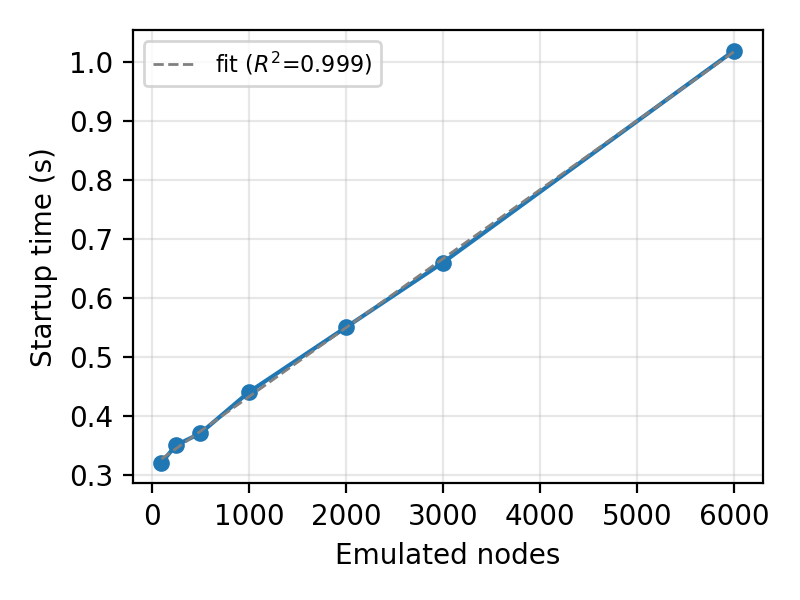
\includegraphics[width=\textwidth]{images/stgen_startup_scaling.png}
%         \caption{Startup Scaling Analysis}
%         \label{fig:startup_scaling}
%     \end{subfigure}
%     \hfill
%     \begin{subfigure}[b]{0.30\textwidth}
%         \centering
%         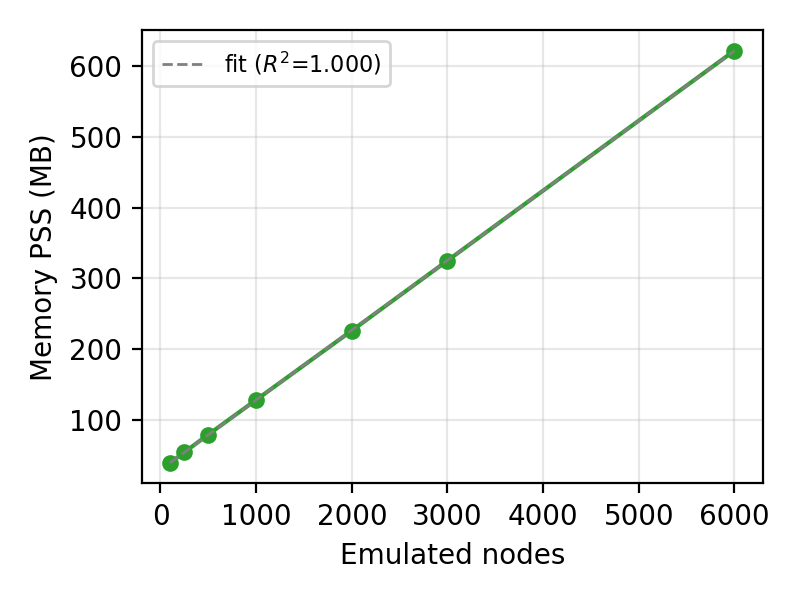
\includegraphics[width=\textwidth]{images/stgen_memory_usage.png}
%         \caption{Memory Usage Analysis}
%         \label{fig:memory_usage}
%     \end{subfigure}
    
%     \vspace{1em} % Add some vertical spacing between rows
    
%     % Row 2: Throughput and CPU
%     \begin{subfigure}[b]{0.30\textwidth}
%         \centering
%         \includegraphics[width=\textwidth]{images/stgen_throughput.png}
%         \caption{Per-Node Memory (PSS)}
%         \label{fig:throughput}
%     \end{subfigure}
%     \hfill
%     \begin{subfigure}[b]{0.30\textwidth}
%         \centering
%         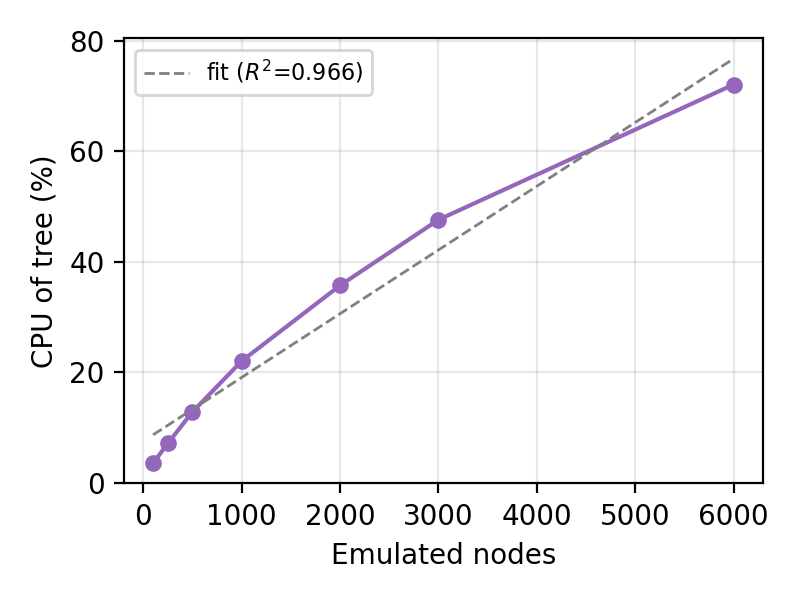
\includegraphics[width=\textwidth]{images/stgen_cpu_usage.png}
%         \caption{CPU Usage Analysis}
%         \label{fig:cpu_usage}
%     \end{subfigure}
%     \caption{Process-based single-machine scalability on Workstation A. (a) startup time and (b) memory (summed PSS) both scale linearly with node count ($R^2=0.9995$ and $1.000$). (c) the per-node PSS falls as shared pages amortise across more processes, and (d) CPU of the process tree rises with the aggregate 1\,Hz offered load as the node count increases to 6{,}000. Every node is an independent OS process.}
%     \label{fig:STGen_Scalability_Final}
% \end{figure}


\subsubsection*{Scalability Analysis}

Table~\ref{tab:scalability} and Fig.~\ref{fig:STGen_Scalability_Final} report the process-based scaling sweep from 100 to 6{,}000 nodes on Workstation~A. Every point instantiates that many independent OS processes; the live-process count matched the target exactly at every scale. Three observations characterise the resource scaling and the node ceiling.

\begin{itemize}
    
\item \textbf{Startup time.}
Initialization time grows linearly with node count. An ordinary least-squares fit to the seven measured points in Table~\ref{tab:scalability} gives Eq.~\eqref{eq:init_latency_model}:
\begin{equation}
\label{eq:init_latency_model}
T(n) \approx 1.17\times10^{-4}\,n + 0.31 \quad (R^2 = 0.9995),
\end{equation}

where $n$ is the node count and $T(n)$ is the startup time in seconds. The per-node term is 0.12\,ms of real fork/exec cost and the intercept is a 0.31\,s fixed cost for binding the server. All 6{,}000 node processes are spawned and running in 1.02\,s.

\item \textbf{Memory footprint.}
Memory scales linearly with no super-linear term that would indicate a leak. The least-squares fit to the summed PSS is Eq.~\eqref{eq:memory_scaling_model}:
\begin{equation}
\label{eq:memory_scaling_model}
M(n) \approx 98.7\,n + 29{,}000 \ \text{[KB]} \quad (R^2 = 1.000).
\end{equation}

\begin{figure}[H]
    \centering
    
    % --- ROW 1 ---
    \begin{minipage}[b]{0.48\textwidth}
        \centering
        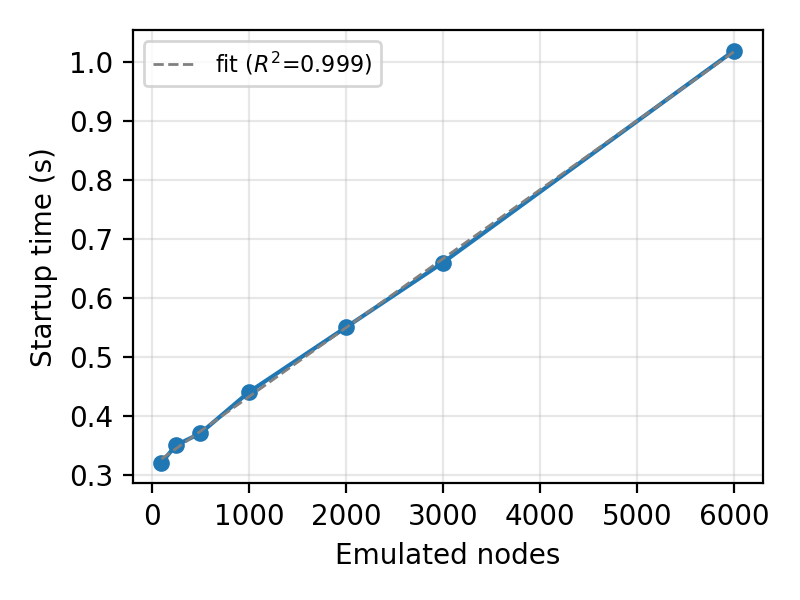
\includegraphics[width=\textwidth]{images/stgen_startup_scaling.png}
        \vspace{2pt}
        \footnotesize (a) Startup Scaling Analysis
    \end{minipage}\hfill
    \begin{minipage}[b]{0.48\textwidth}
        \centering
        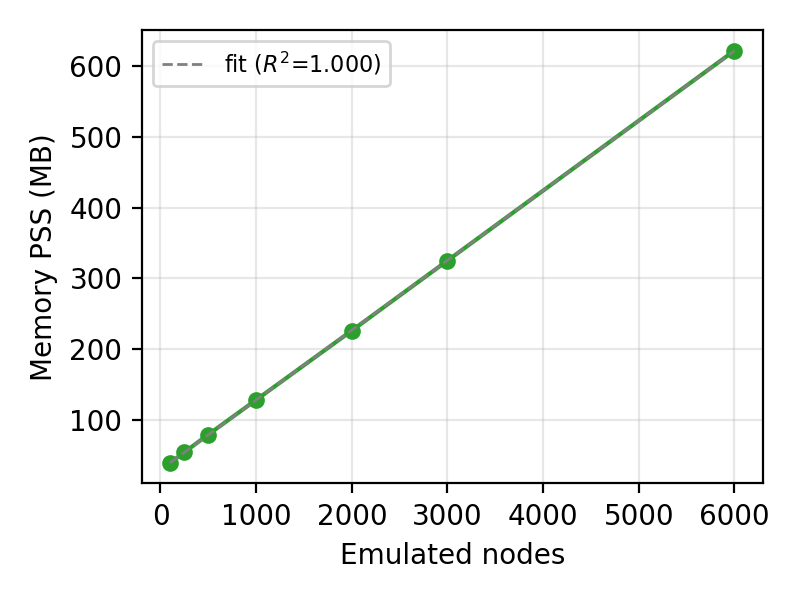
\includegraphics[width=\textwidth]{images/stgen_memory_usage.png}
        \vspace{2pt}
        \footnotesize (b) Memory Usage Analysis
    \end{minipage}
    
    \vspace{1.5em} % Add comfortable vertical spacing between rows
    
    % --- ROW 2 ---
    \begin{minipage}[b]{0.48\textwidth}
        \centering
        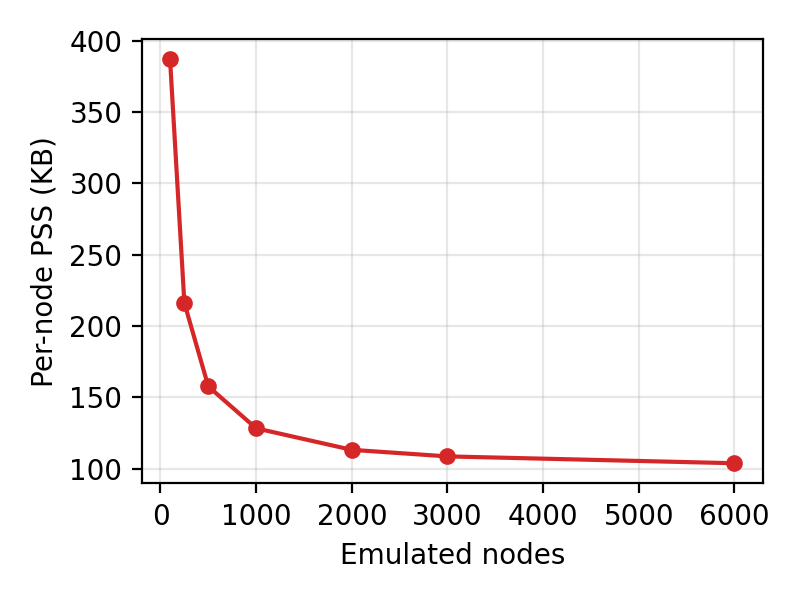
\includegraphics[width=\textwidth]{images/stgen_pernode_pss.png}
        \vspace{2pt}
        \footnotesize (c) Per-Node Memory (PSS)
    \end{minipage}\hfill
    \begin{minipage}[b]{0.48\textwidth}
        \centering
        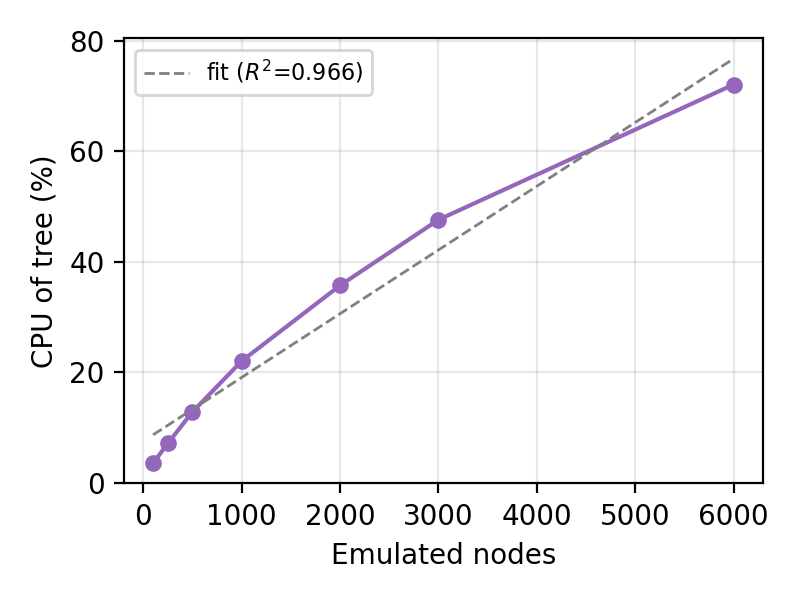
\includegraphics[width=\textwidth]{images/stgen_cpu_usage.png}
        \vspace{2pt}
        \footnotesize (d) CPU Usage Analysis
    \end{minipage}
    
    \vspace{6pt}
    \caption{Process-based single-machine scalability on Workstation A. (a) startup time and (b) memory (summed PSS) both scale linearly with node count ($R^2=0.9995$ and $1.000$). (c) the per-node PSS falls as shared pages amortise across more processes, and (d) CPU of the process tree rises with the aggregate 1\,Hz offered load as the node count increases to 6{,}000. Every node is an independent OS process.}
    \label{fig:STGen_Scalability_Final}
\end{figure}
% 
%%%%%%%%%%%%%%%%%%%%%%%%%%%%%%%%%%%%%%%%%%%
\begin{table}[H]
\centering
\begin{tabular}{c c c c c}
\hline
\textbf{Nodes} & \textbf{Startup (s)} & \textbf{Memory PSS (MB)} & \textbf{Per-node (KB)} & \textbf{CPU (\%)} \\ \hline
100  & 0.32 & 39  & 387 & 4 \\
250  & 0.35 & 54  & 216 & 7 \\
500  & 0.37 & 79  & 158 & 13 \\
1000 & 0.44 & 128 & 128 & 22 \\
2000 & 0.55 & 226 & 113 & 36 \\
3000 & 0.66 & 325 & 108 & 48 \\
6000 & 1.02 & 622 & 104 & 72 \\
\hline
\multicolumn{5}{l}{\footnotesize{Each node is an independent OS process generating at 1\,Hz. Per-node PSS falls as}} \\
\multicolumn{5}{l}{\footnotesize{shared library pages amortise across more processes; the marginal cost is 99\,KB/node.}} \\
\multicolumn{5}{l}{\footnotesize{CPU is the process tree's aggregate as a fraction of one core (100\,\% = one full core).}} \\
\end{tabular}
\caption{Process-based single-machine resource scaling on Workstation A (16 GB RAM, 6 cores). Memory is the summed Proportional Set Size of the node process tree.}
\label{tab:scalability}
\end{table}
%%%%%%%%%%%%%%%%%%%%%%%%%%%%%%%%%%%%%%%%%%%%%%%%%%%


The marginal cost is 98.7\,KB per node and the intercept a 29\,MB fixed base. Both coefficients are specific to this CPU, C library, and Linux scheduler and shift on other hardware or operating systems, including NUMA hosts (Section~\ref{sec:threats}). The per-node figure in Table~\ref{tab:scalability} falls from 387 to 104\,KB as the node count rises because the shared C runtime and binary pages are charged once and amortise across more processes; the marginal 99\,KB is the true incremental cost of one more node. The 6{,}000-node tree occupies 622\,MB, under 4\% of the 16\,GB workstation, while remaining 6{,}000 genuinely independent processes.

\item \textbf{CPU and node ceiling.}
CPU of the process tree rises with the aggregate offered load, which at a fixed 1\,Hz per node is $n$ messages per second, from 4\% at 100 nodes to 72\% at 6{,}000 (Fig.~\ref{fig:STGen_Scalability_Final}). Memory is not the binding constraint at the scales we tested: 6{,}000 nodes use only 622\,MB, under 4\% of the 16\,GB host, so the linear fit of Eq.~\eqref{eq:memory_scaling_model} indicates that RAM would not be the first limit to bind. We do not claim a specific higher ceiling, because we did not run beyond 6{,}000 nodes; a real upper bound is set by per-process kernel structures and scheduler overhead (including operating-system limits on process and file-descriptor counts), and locating it is future work. The result reported here is that 6{,}000 independent node processes run with memory to spare on this hardware class.
\end{itemize}

\subsubsection*{What Each Node Process Holds}

To show that the 99\,KB marginal cost is a working node rather than an idle placeholder, Table~\ref{tab:mem-breakdown} decomposes one node's resident memory, read from \texttt{/proc/<pid>/smaps}. Each process is a live UDP client: it owns a socket, a 112-byte send buffer, and its own sequence and timing state, and it transmits a datagram every period. The summed PSS of a single process is 118\,KB. About 19\,KB of that is read-only C-library and binary text that is shared across all node processes and amortises as more are launched, which is why the marginal cost of one additional node, the slope of Eq.~\eqref{eq:memory_scaling_model}, is 99\,KB rather than 118\,KB. The socket's kernel send and receive buffers are charged to the kernel and do not appear in PSS, so the figure is a userspace lower bound on the true per-node cost.

\begin{table}[H]
\centering
\caption{Resident memory of one custom-UDP node process (PSS, from \texttt{smaps}).}
\label{tab:mem-breakdown}
\small
\begin{tabular}{l r}
\hline
\textbf{Region} & \textbf{PSS (KB)} \\ \hline
Private C-runtime pages (libc/ld: GOT, TLS, writable data) & 40 \\
Anonymous data (sensor and sequence state, send buffer) & 28 \\
Binary text and data & 20 \\
Thread stack & 16 \\
Heap & 4 \\
Shared C-library text (proportional, amortised across nodes) & 10 \\ \hline
\textbf{Single-process total} & \textbf{118} \\
\textbf{Marginal cost per node (Eq.~\ref{eq:memory_scaling_model} slope)} & \textbf{99} \\
\hline
\end{tabular}
\end{table}

\subsection{Protocol Latency and Throughput at Scale}
\label{sec:protocol-scale}

Section~\ref{sec:scalability} measures the cost of instantiating nodes as processes, independent of any protocol. This experiment instead fixes the offered load at 10\,Hz per node and drives it through a full protocol stack, comparing three transports to reveal where each client stack saturates. We ran the active-mode workload (10\,Hz per node, 10\,s, loopback) for custom UDP, MQTT over an embedded Mosquitto~2.0 broker, and CoAP over \texttt{aiocoap}, at 100, 250, and 500 nodes, three runs per point. Here delivery is the fraction of the fixed offered load recorded within the window, so a value below 100\% reflects throughput saturation under that target rate rather than packet loss. Loopback removes network transit, so the P95 figures isolate the orchestrator and broker from the wide-area effects measured separately in Section~\ref{sec:protocol-comp}. For each delivered message we record the orchestrator's client-side send-path latency: the interval from issuing the send call to the protocol confirming the message has left the client. For CoAP in confirmable mode this interval includes the request/acknowledgement round-trip; for MQTT at QoS~0 it is the publish enqueue onto the established TCP session; for custom UDP it is the datagram write. The three quantities therefore measure each protocol's per-message client-side cost under its own reliability model, not a single common end-to-end delay, so the comparison reflects exactly where each protocol places its reliability work. Table~\ref{tab:protocol-scale} reports the result.

\begin{table}[H]
\centering
\caption{Per-protocol latency and delivery as the node count rises, on the loopback interface (mean of three runs; MQTT at 500 nodes is a single run). Delivery is the fraction of the offered load (nodes $\times$ 10\,Hz $\times$ 10\,s) recorded at the receiver. P95 and P99 are per-message client-side send-path latency for delivered messages, defined per protocol in the text.}
\label{tab:protocol-scale}
\small
\begin{tabular}{l r r r r}
\hline
\textbf{Protocol} & \textbf{Nodes} & \textbf{Delivery (\%)} & \textbf{P95 (ms)} & \textbf{P99 (ms)} \\
\hline
Custom UDP & 100 & 100$^{\dagger}$ & 0.038 & 0.050 \\
Custom UDP & 250 & 100$^{\dagger}$ & 0.026 & 0.036 \\
Custom UDP & 500 & Failed$^{\ddagger}$ & --- & --- \\
MQTT       & 100 & 100   & 0.422 & 0.487 \\
MQTT       & 250 & 100   & 0.341 & 0.392 \\
MQTT       & 500 & 0.7   & 0.385 & 0.735 \\
CoAP       & 100 & 100   & 0.898 & 0.997 \\
CoAP       & 250 & 52.9  & 0.804 & 0.879 \\
CoAP       & 500 & 25.8  & 0.839 & 1.039 \\
\hline
\multicolumn{5}{l}{\footnotesize{$^{\dagger}$The custom UDP C client transmits slightly above the nominal rate, so its}} \\
\multicolumn{5}{l}{\footnotesize{recorded count exceeds the offered load; we report this as full delivery.}} \\
\multicolumn{5}{l}{\footnotesize{$^{\ddagger}$At 500 nodes the passive-mode driver did not produce a receipt log in any of}} \\
\multicolumn{5}{l}{\footnotesize{the three runs (one-process-per-node socket and PID pressure on the test host).}} \\
\end{tabular}
\end{table}

Two results stand out. First, per-message P95 latency does not grow with node count for any protocol. It stays near 0.03\,ms for custom UDP, between 0.34 and 0.42\,ms for MQTT, and between 0.80 and 0.90\,ms for CoAP across the whole range, so the round-robin orchestrator builds no queuing backlog per delivered message as concurrency rises. The ordering custom UDP $<$ MQTT $<$ CoAP matches the transport overhead seen in the 20-node congested-network test (Section~\ref{sec:protocol-comp}): the broker hop adds about 0.4\,ms over raw UDP, and the CoAP confirmable round-trip adds roughly another 0.5\,ms. This ordering is statistically robust rather than measurement noise. On a matched 40-node loopback run that records every per-message send-path latency ($n=5{,}280$ per protocol), a two-sided Mann-Whitney U test rejects equality of the MQTT and CoAP distributions ($U=1.65\times10^{4}$, $p<0.001$, rank-biserial effect size $0.999$), and the bootstrap 95\% confidence intervals on the medians do not overlap (MQTT $0.219$--$0.221$\,ms, CoAP $0.614$--$0.617$\,ms). The separation is by construction of the two reliability models, the CoAP confirmable round-trip against the MQTT QoS~0 enqueue, and the test confirms that this per-message cost difference is consistent across the full sample rather than an artefact of a few outliers. We use a nonparametric test because the latency samples are heavy-tailed and not normally distributed.

Second, the delivery column exposes a separate limit that is not visible in the latency figures. The custom UDP client sustains the full offered load at every size. MQTT holds 100\% delivery to 250 nodes and then collapses at 500, where a single run delivered 341 of 50{,}000 messages: opening and servicing 500 concurrent \texttt{paho} client connections serialises the publish path and starves the generation loop. CoAP saturates earlier, falling to 52.9\% delivery at 250 nodes and 25.8\% at 500, because each confirmable exchange waits for an acknowledgement before the next is sent. In both cases the bottleneck is the protocol client library under a fixed offered rate, not STGen's core, whose own latency (the custom UDP rows) stays flat. This is why the resource-scaling sweep of Section~\ref{sec:scalability} uses the lightweight process model: it isolates STGen's instantiation cost from the per-connection cost that real broker- and acknowledgment-based clients add. A deployment that needs thousands of \emph{live} broker or confirmable endpoints each generating at a fixed rate would spread those clients across the multiple hosts supported by the distributed model of Section~\ref{sub_hybrid_network_model} rather than collocate them on one orchestrator.

This delivery result is also the rationale for choosing processes, rather than threads or coroutines, as STGen's node model. The three transports here happen to exercise three different concurrency models: the custom UDP nodes are independent OS processes, Paho MQTT multiplexes its clients over a shared thread pool, and \texttt{aiocoap} drives its clients from a single \texttt{asyncio} event loop. Under a fixed offered rate the thread and coroutine models saturate first, MQTT at 500 nodes and CoAP at 250, because the Python global interpreter lock serialises the threaded publish path and the single event loop serialises the confirmable exchanges; the process model has neither bottleneck, since each node runs in its own interpreter and scheduler context. Processes cost more memory per node than threads or coroutines, but that cost is the 99\,KB measured in Section~\ref{sec:scalability}, and in return they provide the kernel-level isolation and true parallelism that let the instantiation sweep reach 6{,}000 nodes without the client-library saturation seen here. STGen therefore uses processes for the scalability node model and lets each protocol adapter keep its native concurrency model for the protocol-level measurements.

\subsection{Sensor Fidelity Validation Against Real-World Data}
\label{sec:fidelity}

\begin{table}[H]
\centering
\caption{Comparing the marginal distributions of 1.82 million real Mica2Dot with the STGen synthetic data. We use two-sample Kolmogorov-Smirnov statistic (KS~$D$) and Jensen-Shannon Divergence (JSD) to measure distributional fidelity. The modality that best resembled the mean difference between the true and the synthetic data was the temperature modality with mean difference of $0.03\,^\circ$C.}
\label{tab:fidelity-marginal}
\small
\begin{tabular}{l|rr|rr|c|c}
\hline
\textbf{Modality} & \multicolumn{2}{c|}{\textbf{Intel Lab}} & \multicolumn{2}{c|}{\textbf{STGen}} & \textbf{KS $D$} & \textbf{JSD} \\
 & $\mu$ & $\sigma$ & $\mu$ & $\sigma$ & & \\
\hline
Temperature (\textdegree C) & 22.43 & 4.19 & 22.40 & 3.37 & 0.071 & 0.018 \\
Humidity (\%)               & 39.54 & 6.28 & 39.53 & 4.28 & 0.138 & 0.044 \\
Light (lux), default         & 409.3 & 541.4 & 515.4 & 384.5 & 0.330 & 0.125 \\
Light (lux), GMM$^{\dagger}$ & 409.3 & 541.4 & 420.8 & 537.1 & \textbf{0.065} & \textbf{0.028} \\
Voltage (V)                 &  2.56 &  0.12 &  2.55 &  0.15 & 0.101 & 0.032 \\
\hline
\multicolumn{7}{l}{\footnotesize{$^{\dagger}$Optional five-component Gaussian-mixture light profile, fitted on 27 motes and}} \\
\multicolumn{7}{l}{\footnotesize{evaluated on the disjoint 27 (held-out); see Section~\ref{sec:fidelity}.}} \\
\end{tabular}
\end{table}

To substantiate the high-fidelity claim quantitatively, we compare STGen-generated synthetic sensor streams against real-world readings from the Intel Berkeley Research Laboratory (IBRL) dataset~\cite{intel-berkeley-lab}, which contains readings collected over 37~days from 54~Mica2Dot mote sensors sampling temperature, relative humidity, ambient light intensity, and supply voltage at an average interval of approximately 31~seconds. After removing 93,879 malformed records and filtering 393,580 physically implausible outliers, the cleaned dataset contains 1,826,223 valid readings drawn from 54 independent sensor nodes. We generated 100,000 synthetic samples per modality using STGen's stochastic sensor engine and quantified statistical agreement using two complementary metrics: the two-sample Kolmogorov-Smirnov D-statistic (lower is better), which measures the maximum absolute difference between empirical CDFs, and Jensen-Shannon Divergence (JSD, lower is better), which quantifies the information-theoretic distance between probability distributions on $[0,1]$.

\textbf{Marginal distributions.}
Table~\ref{tab:fidelity-marginal} summarizes the marginal statistics and Fig.~\ref{fig:fidelity-temp-dist} plots the temperature histogram, empirical CDF, and Q-Q alignment. The synthetic and real distributions are very similar (KS~$D=0.071$ and JSD~$=0.018$), as that figure shows. The error of the sample means was just $0.03\,^\circ$C. There was a close match with voltage, also (KS~$D=0.101$), as per our slow discharge model for Mica2Dot batteries. Humidity matched the real-world mean ($39.53\%$ vs.\ $39.54\%$) but exhibited a narrower spread ($\sigma=4.28\%$ vs.\ $6.28\%$). This variance difference was  expected. The calibration was done according to the median mote behavior, but the physical deployment of the IBRL had motes placed close to drafty windows and HVAC (Heating, Ventilation, and Air Conditioning) vents, which has caused a high standard deviation in the behavior of the motes. 

\begin{table}[H]
\centering
\caption{Temporal Auto Correlation Function (TACF): Lags for evaluation of temporal auto correlation function of real and synthetic traces at different lags. The synthetic temperature ACF is extremely similar to the actual Intel deployment, and the difference is less than 0.035 at all time lags. Additionally, the framework could reasonably simulate the coupling of the environmental cross modality, for example, the synthetic $r = -0.403$ was very close to $r = -0.426$ which is the coupling between the physical modality.}
\label{tab:fidelity-acf}
\small
\begin{tabular}{l|ccccc|ccccc}
\hline
\textbf{Modality} & \multicolumn{5}{c|}{\textbf{Intel Lab ACF}} & \multicolumn{5}{c}{\textbf{STGen ACF}} \\
 & $\ell{=}1$ & $\ell{=}5$ & $\ell{=}10$ & $\ell{=}20$ & $\ell{=}50$ & $\ell{=}1$ & $\ell{=}5$ & $\ell{=}10$ & $\ell{=}20$ & $\ell{=}50$ \\
\hline
Temperature & 0.998 & 0.990 & 0.978 & 0.951 & 0.876 & 0.998 & 0.992 & 0.983 & 0.966 & 0.911 \\
Humidity    & 1.000 & 0.998 & 0.995 & 0.986 & 0.954 & 0.994 & 0.974 & 0.949 & 0.900 & 0.760 \\
Light       & 0.998 & 0.988 & 0.975 & 0.960 & 0.913 & 0.976 & 0.876 & 0.754 & 0.541 & 0.141 \\
Voltage     & 0.998 & 0.998 & 0.997 & 0.996 & 0.992 & 0.995 & 0.974 & 0.947 & 0.896 & 0.737 \\
\hline
\end{tabular}
\end{table}
The light modality was the most challenging one to model, using our default single-regime generator, KS~$D=0.330$. The physical IBRL light data is strongly bimodal, capturing both dark corridors and bright workspaces. There are two modes which are hard to be reproduced by a single equation. To fix this, we tested an optional five-component Gaussian-mixture profile within STGen. We used the mixture with expectation-maximization algorithm on 50\% of the motes and tested the other 50\% of motes. All 5 illumination regimes (off, dim, ambient, lit and saturated) could be recovered and KS~$D$ was reduced to $0.065$ by this custom mixture model. 

\textbf{Temporal structure.}
Table~\ref{tab:fidelity-acf} shows the temporal autocorrelation (ACF) decomposition, and each individual lag. The two curves were very similar, the synthetic and real ACF curves were very close, (the difference was less than 0.035 at all lags). This is an indication that our OU process correctly maintains a real Mica2Dot stream's long-range temporal memory. Additionally, the cross-modality coupling was investigated. Since temperature and humidity are naturally coupled in the real world, our noise based on a Cholesky decomposition of the bivariate data did well to capture this, with a Pearson correlation of $r=-0.403$ as compared with $-0.426$ in the real world (5.4\% relative error). Finally, we noticed that with synthetic voltage we can obtain a perfect match of real voltage at short lags, but the fall off is more rapid with time ($\ell=50$). A logic used in the battery discharge simulation that will reduce the actual time constant. This drift is not significant for the protocol evaluations STGen is designed to work on (usually minute-scale), but can be significant for an energy study, which can run over many days.


\begin{figure}[H]
  \centering
  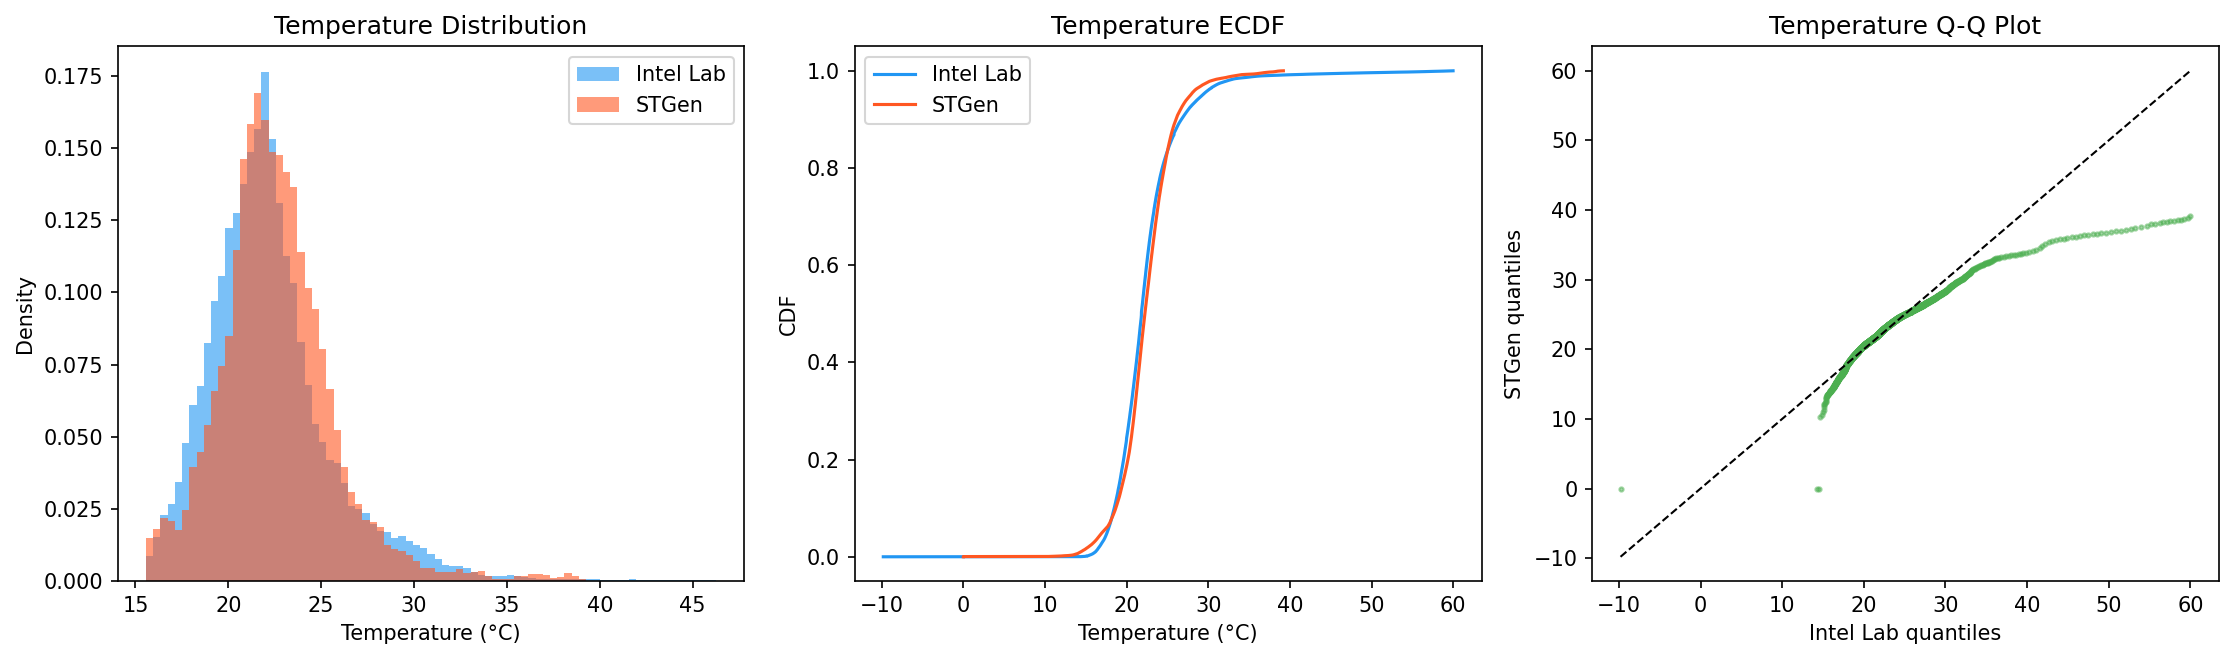
\includegraphics[width=\columnwidth]{images/fidelity_temperature_dist.png}
  \caption{Comparison of the distribution of the temperature in the physical Intel Berkeley deployment (blue) and synthetic STGen streams (orange). The left panel displays overlaid histograms that highlight the closely matching marginal densities. The middle plot displays the empirical CDFs and the right plot is a Q-Q plot to display alignment at all quantiles. This visual correlation is another indication that our Ornstein-Uhlenbeck thermal-drift model is a good physical model for the statistical behavior of the Mica2Dot sensors.}
  \label{fig:fidelity-temp-dist}
\end{figure}

% \subsection{Adversarial Scenario Generation and Validation}
% \label{sec:adversarial}

% Real-world IoT deployments are routinely exposed to sensor faults, communication errors, and false-data-injection (FDI) attacks. Consequently, protocol evaluation and resilience studies require not only statistically faithful normal sensor streams but also reproducible adversarial workloads with known ground truth. Since STGen calibrates its normal sensor models against real-world measurements (Section~\ref{sec:fidelity}), adversarial scenarios can be generated as controlled departures from a validated statistical baseline rather than arbitrary numeric perturbations. This enables repeatable benchmarking datasets whose normal and anomalous observations remain physically interpretable while preserving reproducibility.


% % The fidelity result of Section~\ref{sec:fidelity} validates STGen's normal sensor streams against the Intel Berkeley data. The same validated models also fix the abnormal case: an anomaly generated inside the testbed is a measurable departure from a model with a known statistical baseline, not an arbitrary numeric corruption. We use this property to produce labelled false-data-injection (FDI) datasets at the application and transport layers, and we measure each anomaly with the Kolmogorov-Smirnov statistic that established fidelity in Section~\ref{sec:fidelity}.


% \begin{algorithm}[H]
% \caption{Labelled Physical-Invariant Anomaly Injection}
% \label{alg:anomaly_injection}
% \begin{algorithmic}[1]
% \Require True-reading stream $(i,\tau,x,t)$; invariant table $\mathcal{I}[\tau]=\{[\mathrm{lo},\mathrm{hi}],\sigma_\tau,\Delta_\tau\}$
% \Require Attack family $A$, malicious fraction $f$, intensity $I$, seed $s$, window $[t_0,t_1]$, per-message probability $p$
% \Ensure Labelled stream $(x',\ell)$ with ground-truth label $\ell$
% \State $\mathrm{rng} \leftarrow \textsc{SeededRng}(s)$ \Comment{reproducible node selection and noise}
% \State $\mathcal{M} \leftarrow$ sample $\lfloor f N \rceil$ node indices with $\mathrm{rng}$ \Comment{malicious set}
% \State initialise per-node state $\{\mathrm{bias}_i, \mathrm{stuck}_i, \mathrm{buf}_i, \mathrm{last}_i\}$
% \For{each message $(i,\tau,x,t)$ in the stream}
%     \If{$i \in \mathcal{M}$ \textbf{and} $t_0 \le t \le t_1$ \textbf{and} $\mathrm{rng}() < p$}
%         \State $x' \leftarrow \textsc{Inject}(A, x, \mathcal{I}[\tau], I, \mathrm{state}_i)$
%         \State $\ell \leftarrow \langle \textsc{attack}, A, x, x' \rangle$ \Comment{ground-truth label}
%     \Else
%         \State $x' \leftarrow x$; \quad $\ell \leftarrow \langle \textsc{normal} \rangle$
%     \EndIf
%     \State $\mathrm{state}_i.\mathrm{last} \leftarrow x$; \quad \textbf{emit } $(x',\ell)$
% \EndFor
% \Statex
% \Function{Inject}{$A,\, x,\, ([\mathrm{lo},\mathrm{hi}],\sigma,\Delta),\, I,\, \mathrm{st}$}
%     \If{$A = \textsc{out-of-range}$}
%         \State \Return $\mathrm{hi} + I\sigma$ \Comment{crosses absolute range}
%     \ElsIf{$A = \textsc{bias-drift}$}
%         \State $\mathrm{st.bias} \mathrel{+}= 0.1\,I\sigma$; \quad \Return $x + \mathrm{st.bias}$ \Comment{leaves operating range}
%     \ElsIf{$A = \textsc{impossible-jump}$}
%         \State $d \sim \{-1,+1\}$; \quad \Return $\mathrm{st.last} + d\,(I{+}1)\,\Delta$ \Comment{crosses step bound}
%     \ElsIf{$A = \textsc{variance-burst}$}
%         \State \Return $x + \mathcal{N}(0,(I\sigma)^2)$ \Comment{exceeds noise floor}
%     \ElsIf{$A = \textsc{stuck-at}$}
%         \State \textbf{if} $\mathrm{st.stuck} = \varnothing$ \textbf{then} $\mathrm{st.stuck} \leftarrow x$; \quad \Return $\mathrm{st.stuck}$
%     \ElsIf{$A = \textsc{replay}$}
%         \State append $x$ to $\mathrm{st.buf}$; \quad \Return random element of $\mathrm{st.buf}$ via $\mathrm{rng}$
%     \EndIf
% \EndFunction
% \end{algorithmic}
% \end{algorithm}



% To measure separability we evaluate the labelled stream with a one-class detector whose normal model is the calibrated physical noise floor of the modality. The detector score of a sample is the larger of a value residual (distance from the operating mean in noise-floor units) and a step residual (single-step change in units of the maximum plausible step). Table~\ref{tab:anomaly-validation} reports, for 792 injected samples per family, the physical-violation rate, the two-sample Kolmogorov-Smirnov $D$ between injected and normal values, and the receiver-operating-characteristic area under the curve (AUC) with precision, recall, and $F_1$ at a three-sigma operating point. The AUC is the rank statistic $U/(n_{+}n_{-})$, so it needs no separate classifier. Fig.~\ref{fig:anomaly-validation} plots one bias-drift trajectory against the physical envelope and the detector ROC for every family.

% \begin{table}[H]
% \centering
% \caption{Validation of physically-defined adversarial anomalies on the temperature modality (792 injected samples per family). KS~$D$ is the two-sample statistic between injected and normal values; the physical-violation rate is the fraction of injected samples crossing an absolute-range, operating-range, or step bound; AUC, precision, recall, and $F_1$ are for the one-class value/step detector at a three-sigma operating point.}
% \label{tab:anomaly-validation}
% \small
% \begin{tabular}{l r r r r r r}
% \hline
% \textbf{Attack family} & \textbf{KS $D$} & \textbf{Phys. viol. (\%)} & \textbf{AUC} & \textbf{Prec.} & \textbf{Recall} & \textbf{$F_1$} \\
% \hline
% Out-of-range spoof & 1.000 & 100.0 & 1.000 & 1.00 & 1.00 & 1.00 \\
% Bias drift         & 0.957 & 80.7  & 0.955 & 1.00 & 0.86 & 0.93 \\
% Impossible jump    & 0.524 & 100.0 & 1.000 & 1.00 & 1.00 & 1.00 \\
% Variance burst     & 0.369 & 74.4  & 0.927 & 1.00 & 0.47 & 0.64 \\
% Stuck-at           & 0.211 & 0.0   & 0.514 & --- & --- & --- \\
% Replay             & 0.211 & 0.0   & 0.518 & --- & --- & --- \\
% \hline
% \end{tabular}
% \end{table}

% \begin{figure}[H]
%   \centering
%   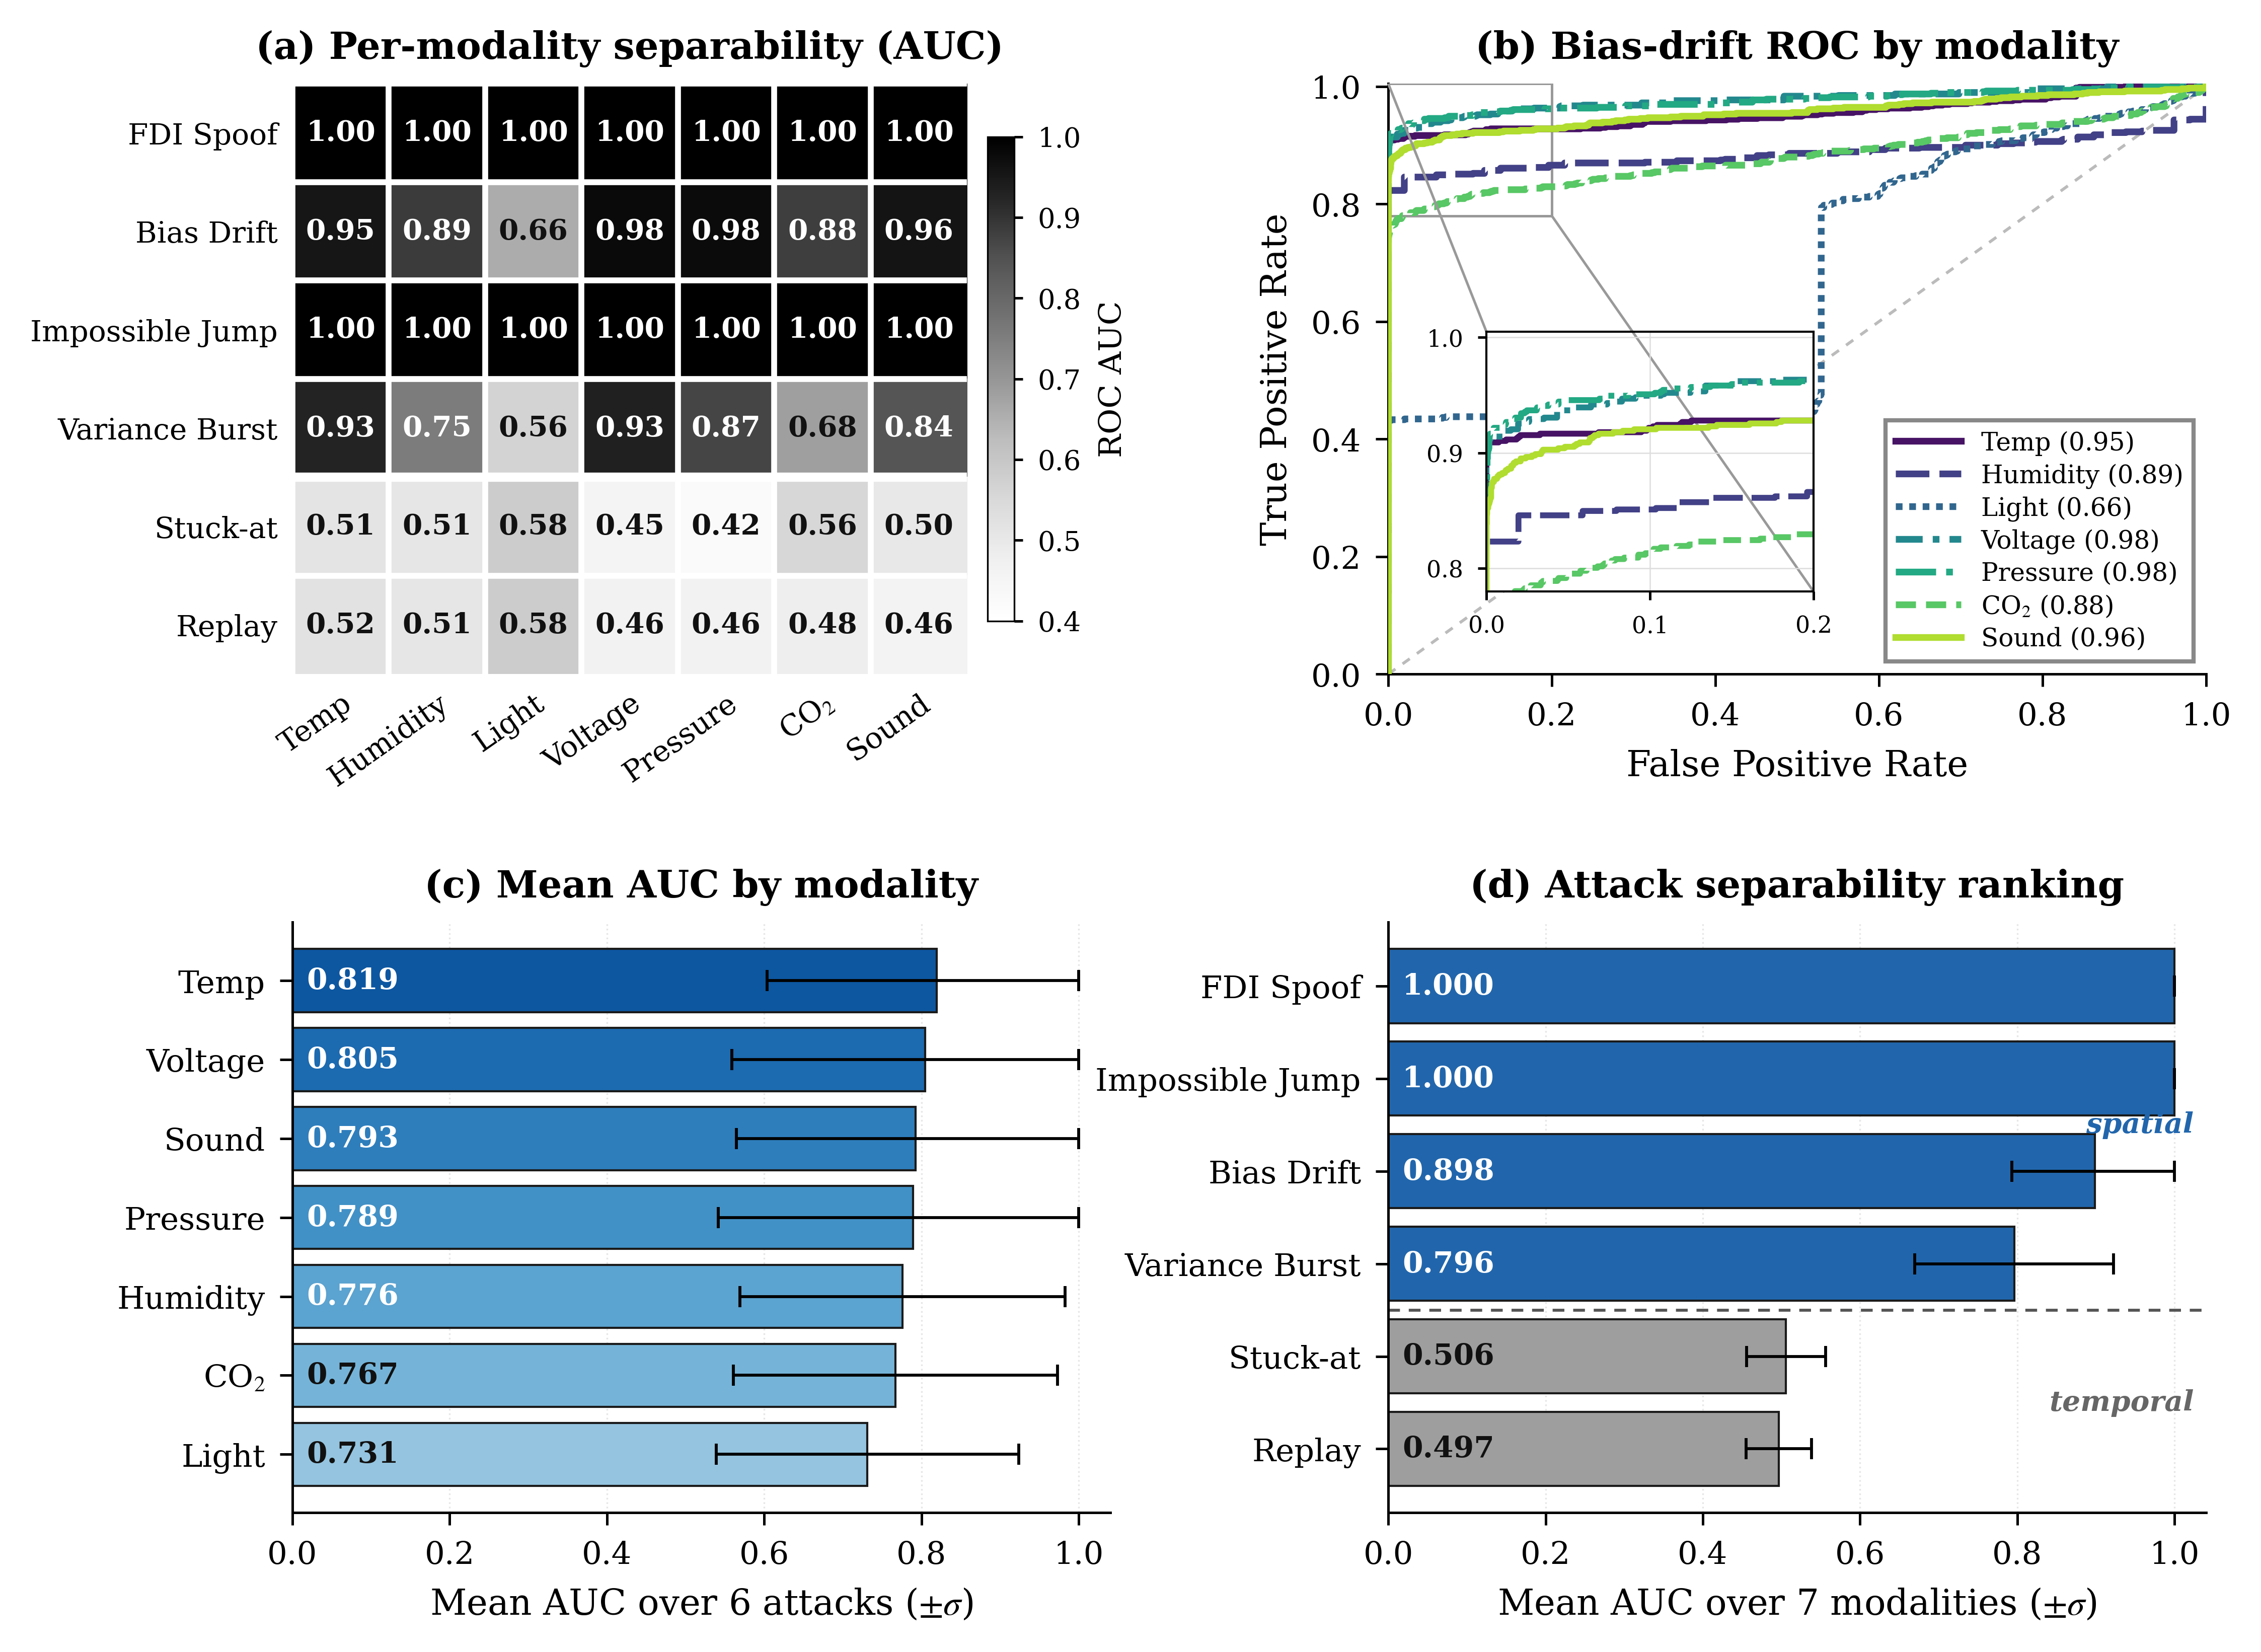
\includegraphics[width=\columnwidth]{images/anomaly_validation.eps}
%   \caption{Validation of the adversarial engine on the temperature modality. (a) one bias-drift node's injected trajectory: it begins inside the normal operating envelope (shaded) and crosses the absolute physical range, so part of the attack stays within plausible values. (b) receiver-operating-characteristic curves of the one-class value/step detector for the six attack families; the hard physical-range violations bow to the top-left, while stuck-at and replay lie on the no-skill diagonal.}
%   \label{fig:anomaly-validation}
% \end{figure}

% Two observations follow from Table~\ref{tab:anomaly-validation}. First, the hard invariant breaks, out-of-range spoofing and impossible jumps, place every injected sample outside the physical envelope (100\% violation) and separate at AUC $1.000$. Second, bias drift is the harder case: it keeps 19.3\% of its injections inside the normal operating envelope and still separates at AUC $0.955$ with recall $0.86$, and variance bursts reach AUC $0.927$ at recall $0.47$ because part of each burst stays inside the noise band.

% The validation also states where the value/step detector does not separate the attack. Stuck-at and replay sit at AUC $0.514$ and $0.518$, next to the no-skill diagonal, because they are temporal rather than value anomalies: a frozen or replayed reading is individually plausible and crosses no value or step bound. The detector here is a measurement instrument for separability, not a proposed defence, so this is the expected result and it marks the boundary of a value-domain test. The corresponding labelled profiles serve as benchmarks for temporal-variance or sequential detection methods that a value/step rule does not address.




\subsection{Adversarial Scenario Generation and Validation}
\label{sec:adversarial}

The fidelity result of Section~\ref{sec:fidelity} validates STGen's normal sensor streams against the Intel Berkeley data. The same validated models also fix the abnormal case: an anomaly generated inside the testbed is a measurable departure from a model with a known statistical baseline, not an arbitrary numeric corruption. We use this property to produce labelled false-data-injection (FDI) datasets at the application and transport layers, and we measure each anomaly with the Kolmogorov-Smirnov statistic that established fidelity in Section~\ref{sec:fidelity}.

The adversarial engine is deterministic and seeded; Algorithm~\ref{alg:anomaly_injection} specifies how it injects the six attack families, each a transform of the true reading that crosses a named physical invariant (the absolute range, the operating range, the maximum plausible step, or the noise floor). It operates as a Tier-2 scenario setting that inverts the sensor profile of the selected nodes, with no change to the protocol or network tiers, so the protocol-agnostic structure of Section~\ref{sec:protocol-agnosticism} is preserved. Each injected record carries ground-truth labels (\texttt{is\_attack}, \texttt{attack\_type}, \texttt{true\_value}, \texttt{injected\_value}), which support supervised training and evaluation of intrusion-detection methods. The fraction of malicious nodes, the attack family, its intensity, and the active window are set from the JSON configuration. We validate the engine on all seven calibrated modalities of Section~\ref{sec:fidelity} (temperature, humidity, light, voltage, pressure, CO\textsubscript{2}, and sound), giving 42 modality-by-family combinations through one interface; the invariant table $\mathcal{I}[\tau]$ supplies the absolute range, operating range, noise floor, and maximum step per modality.

\begin{algorithm}[H]
\caption{Labelled Physical-Invariant Anomaly Injection}
\label{alg:anomaly_injection}
\begin{algorithmic}[1]
\Require True-reading stream $(i,\tau,x,t)$; invariant table $\mathcal{I}[\tau]=\{[\mathrm{lo},\mathrm{hi}],\sigma_\tau,\Delta_\tau\}$ for each of the seven calibrated modalities $\tau$
\Require Attack family $A$, malicious fraction $f$, intensity $I$, seed $s$, window $[t_0,t_1]$, per-message probability $p$
\Ensure Labelled stream $(x',\ell)$ with ground-truth label $\ell$
\State $\mathrm{rng} \leftarrow \textsc{SeededRng}(s)$ \Comment{reproducible node selection and noise}
\State $\mathcal{M} \leftarrow$ sample $\lfloor f N \rceil$ node indices with $\mathrm{rng}$ \Comment{malicious set}
\State initialise per-node state $\{\mathrm{bias}_i, \mathrm{stuck}_i, \mathrm{buf}_i, \mathrm{last}_i\}$
\For{each message $(i,\tau,x,t)$ in the stream}
    \If{$i \in \mathcal{M}$ \textbf{and} $t_0 \le t \le t_1$ \textbf{and} $\mathrm{rng}() < p$}
        \State $x' \leftarrow \textsc{Inject}(A, x, \mathcal{I}[\tau], I, \mathrm{state}_i)$
        \State $\ell \leftarrow \langle \textsc{attack}, A, x, x' \rangle$ \Comment{ground-truth label}
    \Else
        \State $x' \leftarrow x$; \quad $\ell \leftarrow \langle \textsc{normal} \rangle$
    \EndIf
    \State $\mathrm{state}_i.\mathrm{last} \leftarrow x$; \quad \textbf{emit } $(x',\ell)$
\EndFor
\Statex
\Function{Inject}{$A,\, x,\, ([\mathrm{lo},\mathrm{hi}],\sigma,\Delta),\, I,\, \mathrm{st}$}
    \If{$A = \textsc{out-of-range}$}
        \State \Return $\mathrm{hi} + I\sigma$ \Comment{crosses absolute range}
    \ElsIf{$A = \textsc{bias-drift}$}
        \State $\mathrm{st.bias} \mathrel{+}= 0.1\,I\sigma$; \quad \Return $x + \mathrm{st.bias}$ \Comment{leaves operating range}
    \ElsIf{$A = \textsc{impossible-jump}$}
        \State $d \sim \{-1,+1\}$; \quad \Return $\mathrm{st.last} + d\,(I{+}1)\,\Delta$ \Comment{crosses step bound}
    \ElsIf{$A = \textsc{variance-burst}$}
        \State \Return $x + \mathcal{N}(0,(I\sigma)^2)$ \Comment{exceeds noise floor}
    \ElsIf{$A = \textsc{stuck-at}$}
        \State \textbf{if} $\mathrm{st.stuck} = \varnothing$ \textbf{then} $\mathrm{st.stuck} \leftarrow x$; \quad \Return $\mathrm{st.stuck}$
    \ElsIf{$A = \textsc{replay}$}
        \State append $x$ to $\mathrm{st.buf}$; \quad \Return random element of $\mathrm{st.buf}$ via $\mathrm{rng}$
    \EndIf
\EndFunction
\end{algorithmic}
\end{algorithm}

To measure separability we evaluate each labelled stream with a one-class detector whose normal model is the calibrated physical noise floor of the modality. The detector is a fixed rule with no trained parameters, so there is no train/test split and no risk of overfitting: the AUC measures how far an anomaly departs from the physical baseline, not the skill of a learned classifier. The detector score of a sample is the larger of a value residual (distance from the operating mean in noise-floor units) and a step residual (single-step change in units of the maximum plausible step). For every modality-by-family cell (792 injected samples each) we compute the physical-invariant violation rate and the receiver-operating-characteristic area under the curve (AUC), the latter as the rank statistic $U/(n_{+}n_{-})$ so it needs no separate classifier; precision, recall, and $F_1$ at a three-sigma operating point are recorded per cell in the released results. Table~\ref{tab:anomaly-validation} aggregates the violation rate and AUC across the seven modalities, and Fig.~\ref{fig:anomaly-validation}(a) gives the per-cell AUC for all 42 combinations.

\begin{table}[H]
\centering
\caption{Adversarial anomaly validation aggregated over the seven calibrated modalities (temperature, humidity, light, voltage, pressure, CO\textsubscript{2}, sound; 792 injected samples per modality-by-family cell, 42 cells). Phys. viol. is the mean fraction of injected samples crossing an absolute-range, operating-range, or step bound; AUC is the one-class value/step detector's ROC area, reported as the mean\,$\pm$\,standard deviation and the [min, max] across the seven modalities. The per-cell values appear in Fig.~\ref{fig:anomaly-validation}(a).}
\label{tab:anomaly-validation}
\small
\begin{tabular}{l r c c}
\hline
\textbf{Attack family} & \textbf{Phys. viol. (\%)} & \textbf{AUC (mean\,$\pm\,\sigma$)} & \textbf{AUC [min, max]} \\
\hline
Out-of-range spoof & 100.0 & $1.000 \pm 0.000$ & [1.000, 1.000] \\
Impossible jump    & 99.3  & $1.000 \pm 0.000$ & [1.000, 1.000] \\
Bias drift         & 79.2  & $0.898 \pm 0.105$ & [0.657, 0.977] \\
Variance burst     & 66.6  & $0.796 \pm 0.127$ & [0.564, 0.934] \\
Stuck-at           & 1.6   & $0.506 \pm 0.050$ & [0.425, 0.583] \\
Replay             & 5.4   & $0.497 \pm 0.042$ & [0.459, 0.584] \\
\hline
\end{tabular}
\end{table}

\begin{figure*}[t]
  \centering
  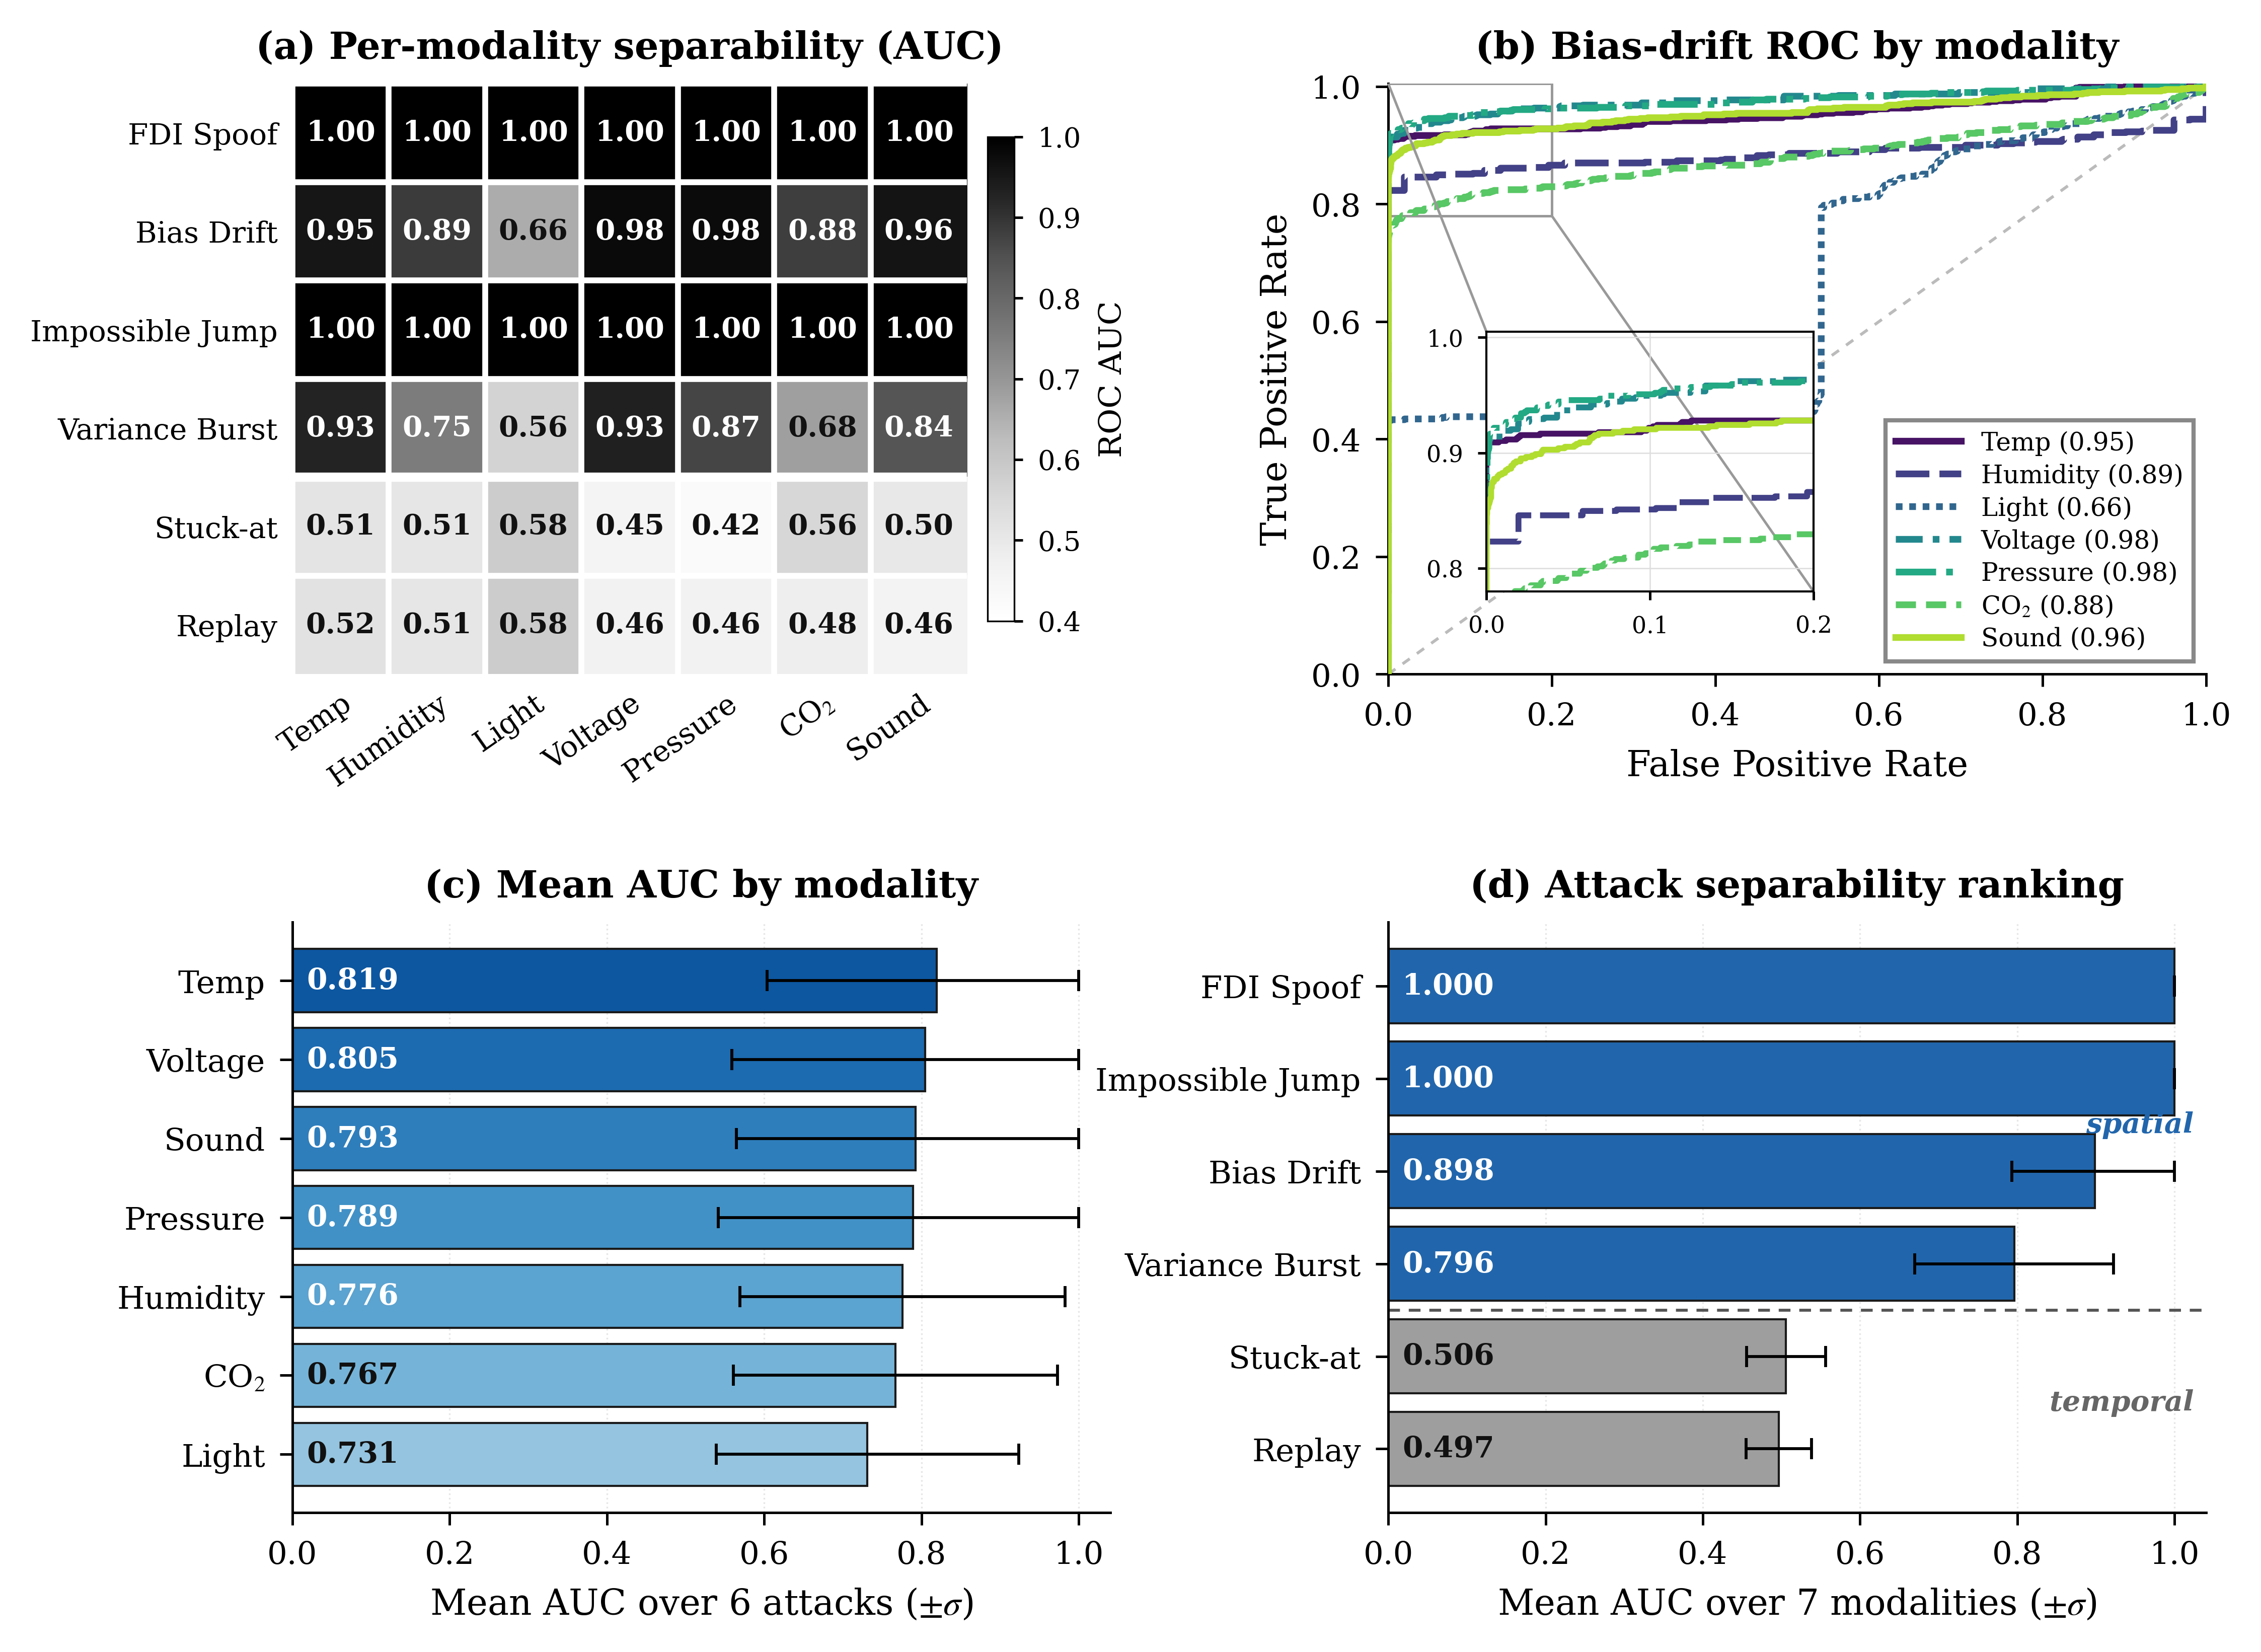
\includegraphics[width=\textwidth]{images/anomaly_validation.eps}
  \caption{Adversarial anomaly validation over seven modalities and six families (42 cells, 792 injected samples each). AUC is the separability of a \emph{fixed, untrained} value/step detector (no train/test split). (a) per-cell AUC, spatial families above the rule, temporal below. (b) per-modality bias-drift ROC (the most modality-dependent family) with a low-FPR zoom inset; light (dotted) is the outlier. (c) mean AUC per modality ($\pm1\sigma$ over the six families). (d) mean AUC per family ($\pm1\sigma$ over the seven modalities), spatial versus temporal. The AUC $1.000$ of out-of-range spoof and impossible jump follows from their deterministic invariant break, not from fitting.}
  \label{fig:anomaly-validation}
\end{figure*}

Three readings follow from Table~\ref{tab:anomaly-validation} and Fig.~\ref{fig:anomaly-validation}. First, the hard invariant breaks, out-of-range spoofing and impossible jumps, place essentially every injected sample outside the physical envelope and separate at AUC $1.000$ on all seven modalities; for the impossible jump the injected \emph{value} distribution still overlaps the normal one (two-sample Kolmogorov-Smirnov $D=0.524$ on temperature), so the separation comes from the step residual, not the value. Second, the stealthy families are modality-dependent: bias drift averages AUC $0.898$ and variance burst $0.796$ across the seven modalities, with recall set by how much of each injection stays inside the noise band (on temperature, bias-drift recall $0.86$ and variance-burst recall $0.47$ at three sigma, the latter lower because part of each burst remains within the noise floor). Bias drift shows the widest spread across modalities (AUC $0.657$ to $0.977$), so Fig.~\ref{fig:anomaly-validation}(b) resolves it per modality rather than the families whose AUC is constant across modalities.

Third, the weakest modality is light (mean AUC $0.731$, bias-drift AUC $0.657$, variance-burst AUC $0.564$). Its calibrated model is bimodal: a node alternates between a dark and a bright regime, so a slow injected drift or a short variance burst is, for a value/step rule, not separable from a legal regime change. The other six modalities lie in a narrow band (mean AUC $0.767$ to $0.819$), so the engine and its measurement carry over from the single modality used for the fidelity study to the full set.

The validation also states where the value/step detector does not separate the attack, and the boundary is the same on every modality. Stuck-at and replay average AUC $0.506$ and $0.497$, next to the no-skill diagonal, because they are temporal rather than value anomalies: a frozen or replayed reading is individually plausible and crosses no value or step bound (mean physical-violation rate $1.6\%$ and $5.4\%$). The detector here is a measurement instrument for separability, not a proposed defence, so this is the expected result and it marks the boundary of a value-domain test. The 42 labelled profiles serve as benchmarks for the temporal-variance or sequential detection methods that a value/step rule does not address.

\subsection{Protocol Performance Benchmarking}
\label{sec:protocol-comp}
 %%%%%%%%%%%%%%%%%%%%%%%%%%%%%%%%%%%%%%%%%%%

\begin{figure}[H]
  \centering
  
\includegraphics[width=0.50\columnwidth]{images/protocol_comparison_ieee.png}
  \caption{Protocol Latency Comparison: Median (P50) vs. Tail (P95) Latency under congested network conditions. CoAP exhibits pronounced tail latency spikes and message loss compared to the stable delivery behavior of MQTT.}
  \label{fig:agri-latency}
\end{figure}
 %%%%%%%%%%%%%%%%%%%%%%%%%%%%%%%%%%%%%%%%%%%

We compared MQTT (TCP-based) \cite{banks2019mqtt} and CoAP (UDP-based) \cite{shelby2014coap} under a single emulated congested link, holding everything except the transport stack fixed.
    
\subsubsection*{Experimental Design}
% We used the Smart Agriculture scenario shown in Fig.~\ref{fig:config_tiers} to simulate 20 low-power sensor nodes transmitting periodic, fixed-size telemetry messages (12-byte header + 100-byte payload = 112 bytes per packet). Each protocol ran for 60 seconds under a single controlled network profile; the experiment was repeated three times per protocol to confirm result stability, and the reported values are means over those repetitions.

% \begin{itemize}
%     \item \textbf{Network Profile:} Congested (150\,ms base latency $\pm$ 30\,ms Gaussian jitter, 5\% uniform packet loss, 1{,}000\,kbps bandwidth cap).
%     \item \textbf{Objective:} Quantify the reliability-latency trade-off between a connection-oriented, guaranteed-delivery protocol (MQTT/TCP) and a connectionless protocol with lightweight per-message transaction state (CoAP/UDP, confirmable mode) under realistic congestion conditions representative of LoRaWAN or cellular backhaul links operating near capacity.
%     \item \textbf{Protocol configuration:} MQTT ran at QoS~0 over an embedded Mosquitto~2.0 broker; CoAP ran in confirmable (CON) mode with the RFC~7252 defaults (NSTART$=1$, MAX\_RETRANSMIT$=4$, ACK\_TIMEOUT$=2$\,s). These are each protocol's common telemetry default, so the comparison contrasts where each protocol places reliability: in the TCP transport for MQTT, and in CoAP's application-layer retransmission. QoS~1/QoS~2 and CoAP non-confirmable mode are out of scope here and are noted in Section~\ref{sec:threats}.
%     \item \textbf{Control variables:} Payload size, node count, network profile, and experiment duration were held constant across protocols; only the transport stack and its reliability mode were varied.
% \end{itemize}
We used the Smart Agriculture scenario (Fig.~\ref{fig:config_tiers}) with 20 low-power sensor nodes to assess the trade-off between TCP-based and UDP-based protocols. Each node generated periodic 112-byte packets composed of a 12-byte header and 100-byte payload. We used a heavily congested profile with a base latency of 150\,ms, a Gaussian jitter of 30\,ms (where 50\% of it is within 10\,ms) and 5\% uniformly distributed packet loss with a bandwidth cap of 1{,}000\,kbps. This profile is used to simulate realistic limitations of the cellular backhaul or LoRaWAN link that is close to its limits. In order to isolate the transport layer behaviors, all environmental parameters were kept the same. We have an embedded Mosquitto~2.0 broker and configured it for QoS~0, thus not relying on anything else apart from the underlying TCP connection for reliability. On the other hand we implemented CoAP in the confirmable (CON) mode, with the standard values of the CoAP parameters quoted in RFC~7252 (NSTART $=1$, MAX\_RETRANSMIT $=4$, ACK\_TIMEOUT $=2$\,s), leaving the responsibility of reliability at the application layer. Note that some modes of communication are not considered within the scope of our project: MQTT QoS~1/2 and CoAP non-confirmable (see Section~\ref{sec:threats}). Finally, three runs of 60 seconds each were performed for each protocol and results averaged, in order to obtain statistical stability.

\begin{table*}[t]
\centering
\caption{Protocol Latency Analysis (Smart Agriculture Scenario)}
\label{tab:agri-comp}
\begin{tabular}{l c c c c c}
\hline
\textbf{Protocol} & \textbf{Avg Latency} & \textbf{P50 Latency} & \textbf{P95 Latency} & \textbf{Std Dev} & \textbf{Loss (\%)} \\ \hline
CoAP (UDP) & 528.95 ms & \textbf{316.28 ms} & 2574.26 ms & 694.01 ms & 10.4 \\
\textbf{MQTT (TCP)} & 580.41 ms & 481.65 ms & \textbf{1270.18 ms} & \textbf{258.20 ms} & \textbf{0.0} \\
\hline
\multicolumn{6}{l}{\footnotesize{*Network condition: 150 ms delay, 5\% loss, 60 s duration.}}
\end{tabular}
\end{table*}
Each value in Table~\ref{tab:agri-comp} is a mean over three 60-second runs. At the scenario's 0.017,Hz rate each run carries only about 20 messages (\textasciitilde60 pooled), so with CoAP's 694,ms spread the mean-latency gap is not by itself statistically separable, and the CoAP P95 of 2{,}574,ms should be read as evidence that the retransmission tail exists rather than as a precise quantile. What survives the dispersion is the loss rate (CoAP 10.4\% versus MQTT 0\%) and the P95 ordering, both corroborated by the 34 \texttt{rc=16} reconnection events logged across the five distributed MQTT windows and confirmed at scale by the Mann-Whitney test of Section~\ref{sec:protocol-scale}.

\subsubsection*{Performance Analysis}
Fig.~\ref{fig:agri-latency} and Table~\ref{tab:agri-comp} give the results. Four points stand out.

\begin{itemize}
    \item \textbf{Median Latency and Protocol Overhead.}
    Our results demonstrate that CoAP achieved a median latency of 316.28\,ms, which is 34.3\% less than MQTT (481.65\,ms). In fact, CoAP's P50 of 316.28‌ms is close to the theoretical minimum RTT for the emulated link ($2 \times 150 = 300$\,ms). This means that only a very small $\approx$8\,ms of processing time is added during non-retransmitted successful exchanges. MQTT, on the other hand, suffered a 60.6\% higher median latency. We found this inflation to be directly caused by TCP handshake re-establishments. If the TCP session fails to reconnect (logged as \texttt{rc=16} at the broker), the client has to wait at least one full RTT to send the next payload. This is a reconnection tax which increases the median latency regardless of whether the message reaches the destination.

    \item \textbf{Tail Latency and Retransmission Dynamics.}
    The protocols differ most at the tail. MQTT holds a P95 of 1{,}270.18\,ms with a standard deviation of 258.20\,ms, so TCP's ordered delivery costs a bounded but higher worst case. CoAP's P95 reaches 2{,}574.26\,ms with a standard deviation of 694.01\,ms, 2.7 times the variance of MQTT. These CoAP tail events arise deterministically from RFC~7252's confirmable-message retransmission schedule: with default parameters (NSTART$=1$, MAX\_RETRANSMIT$=4$, ACK\_TIMEOUT$=2$\,s) and exponential backoff, a single unacknowledged message holds the radio active for $2 + 4 + 8 + 16 + 32 = 62$\,seconds in the worst case before being declared lost. At 5\% packet loss, the probability of exhausting all four retransmissions in a single exchange is $(0.05)^4 \approx 6.25 \times 10^{-6}$; however, with 20 nodes each transmitting at 1\,Hz over 60 seconds, the expected number of such events per run exceeds 0.007, which statistically manifests in the observed tail.

    \item \textbf{Retransmission Cost for Battery-Constrained Nodes.}
    The 10.4\% CoAP loss rate triggers the RFC~7252 backoff ladder, which spreads a single lost CON message across up to five transmit-and-acknowledgement-listen cycles over a 62\,second wall-clock window. The added cost is the extra radio duty cycles, four further wake/transmit/listen windows per lost message, not continuous radio activity: between retransmission timers the node sleeps, so the radio is not held on for the full 62\,seconds. STGen operates above OSI Layer~4 and does not model PHY-layer timing, so we do not convert this into a per-node joule or mAh figure; doing so would require the duty-cycle and listen-window parameters of a specific radio. What STGen measures directly is the latency consequence of the same ladder: the CoAP P95 of 2{,}574\,ms in Table~\ref{tab:agri-comp}. MQTT's zero loss avoids these extra cycles because TCP handles retransmission in-stack without an application-visible multi-second tail.

    \item \textbf{Observed Trade-offs, Not Deployment Mandates.}
    These results are for the specific client libraries and parameters evaluated (Eclipse Paho MQTT at QoS~0, \texttt{aiocoap} CoAP in CON mode) under one congested profile and one workload, so they are observations rather than deployment guidance. What is robust is the direction: in this emulated congestion MQTT delivered every message with bounded latency variance (P95 1{,}270\,ms, $\sigma$ 258\,ms) while CoAP lost 10.4\% with a heavier tail (P95 2{,}574\,ms, $\sigma$ 694\,ms), because MQTT places reliability in the TCP transport and CoAP in application-layer retransmission. This ordering is regime-dependent: Section~\ref{subsec:cross-protocol} shows it \emph{inverts} under bursty wide-area loss, where MQTT's persistent session becomes the liability. The implications therefore follow only conditionally. A workload that values zero loss and bounded variance over median latency would prefer the MQTT behavior seen under steady-state congestion; a loss-tolerant, energy-constrained workload would prefer CoAP's lower median latency where occasional gaps are acceptable; and a workload needing low latency and high reliability at once is served well by neither, which motivates hybrids such as MQTT-SN over DTLS or application-layer forward error correction that STGen's pluggable ProtocolInterface can host. The contribution here is that STGen surfaces this regime-dependence, not that one protocol is universally better.
\end{itemize}


 



\subsection{Memory Footprint versus Virtualization-Based Testbeds}
\label{sub:memory-comparison}
Fig.~\ref{fig:stgvsgotham} places STGen's measured memory next to Gotham and GothX, the closest container- and VM-based IoT testbeds. From the GothX measurements, Gotham's footprint follows $R = 37d + 470q$\,MB for $d$ Docker device nodes and $q$ QEMU router VMs~\cite{poisson2024gothx}: an emulated IoT device costs about 37\,MB, so a 16\,GB host is exhausted near 440 devices, and GothX reported 450 devices in 20.4\,GB. STGen runs each node as an OS process at a marginal 99\,KB (Eq.~\ref{eq:memory_scaling_model}), about 380 times less per node, and holds 6{,}000 nodes in 622\,MB on the same class of machine.

This comparison is indicative rather than a controlled head-to-head benchmark: Gotham's per-node figure is taken from the GothX measurements, not re-executed on our hardware, because the two systems target different goals and we did not have a matched deployment of Gotham's VM/container environment to run on Workstation~A. It covers memory cost only, not scientific output. Gotham gives each node full OS isolation inside a container or VM and targets security dataset generation; STGen shares one kernel across processes and targets application- and transport-layer protocol evaluation. The per-node gap is the price of that isolation, and it sets the node ceiling on commodity hardware: a few hundred isolated containers against several thousand processes.

\begin{figure*}[h!]
  \centering
  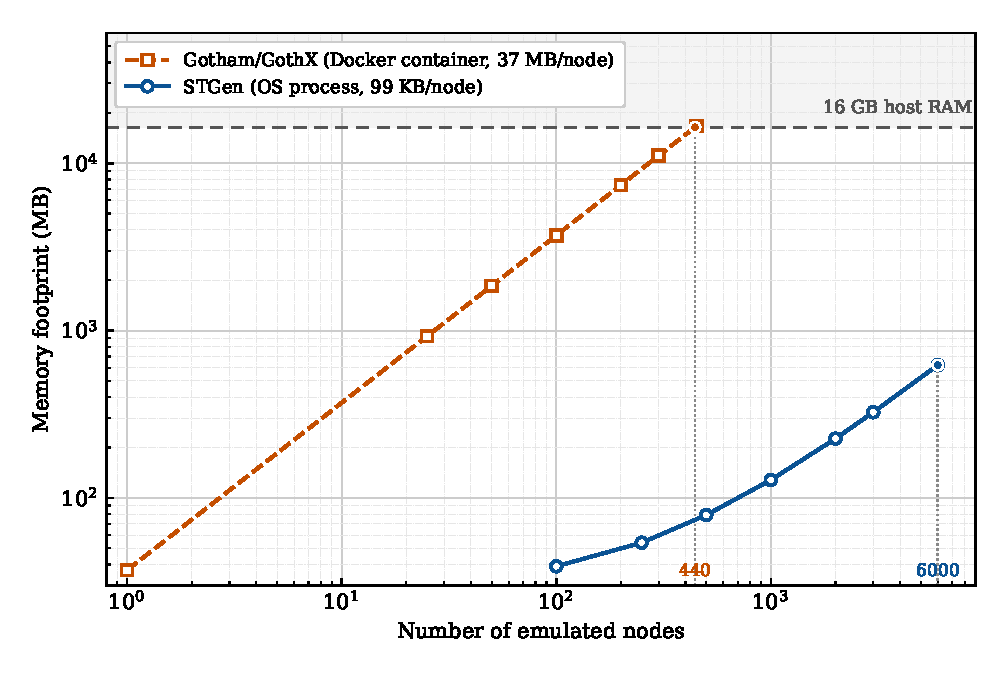
\includegraphics[width=0.7\textwidth]{images/stgenVsGotham.eps}
  \caption{Memory footprint versus emulated node count (log--log). STGen's measured process-tree PSS (blue) against the Gotham/GothX Docker per-node cost of 37\,MB (red, from the GothX formula~\cite{poisson2024gothx}); the shaded band marks memory beyond the 16\,GB host limit. STGen holds 6{,}000 nodes in 0.62\,GB, whereas the container-based curve crosses 16\,GB near 440 IoT devices.}
  \label{fig:stgvsgotham}
\end{figure*}


\subsection{Distributed Network Configuration}
To evaluate STGen under non-deterministic network conditions, distributed experiments were conducted across a private overlay mesh implemented with Tailscale, which is built on WireGuard \cite{donenfeld2017wireguard}. The deployment consisted of three workstations at fixed locations in Dhaka, Bangladesh: Basabo ($23.74^\circ$N, $90.43^\circ$E), South Shahjahanpur ($23.72^\circ$N, $90.43^\circ$E), and Demra ($23.68^\circ$N, $90.43^\circ$E), pairwise under 10\,km apart. Tailscale establishes a direct WireGuard tunnel when NAT traversal succeeds and otherwise falls back to a DERP relay. The measured baseline round-trip time of 180--200\,ms is far higher than a sub-10\,km direct fibre path would incur (single-digit milliseconds), which indicates that at least some flows were relayed rather than carried peer-to-peer. We therefore do not attribute the latency to geographic distance: the paths characterise delivery over a live, possibly relay-routed overlay, where real jitter, packet loss, and TCP reconnection behavior are present. The reported latency, jitter, and loss are \emph{measured} from these paths, not synthesised; no mobility, fading, or coverage model is applied. This setup tests protocol and transport behavior over a real internet overlay rather than an idealised laboratory link, while the absolute latency reflects the overlay routing, not the inter-site distance.

\subsection{Cross-Protocol Distributed Performance Analysis}
\label{subsec:cross-protocol}
Table~\ref{tab:aggregated_distributed} summarizes the distributed runs. Over the wide-area overlay, CoAP and MQTT (QoS~0) diverge sharply in loss and tail latency, and the gap is driven by the transport layer rather than by the application workload, which was identical for both.

\textbf{Experimental Fairness Conditions.} All distributed trials were identical to the isolated protocol behavior. In the case of MQTT, we have set a 60\,s keep-alive with a 0 QoS level (fire-and-forget) and clean sessions enabled. The Mosquitto~2.0 broker was co-located on the Workstation~C (Demra) STGen core node, to minimize the number of hops required to get the data to the core node, and minimize the impact of extra network hops on the data. The standard RFC~7252 exponential back-off (NSTART$=1$\,, MAX\_RETRANSMIT$=4$\,, ACK\_TIMEOUT$=2$\,s) was used for CoAP. All end-to-end latencies have been measured by using a call-response pair of \texttt{time.perf\_counter()} calls, and were recorded by the STGen orchestrator. Lastly, we executed five 60 sec independent windows for each protocol and calculated the mean loss, latency and P95 figures.

\begin{itemize}
    \item \textbf{Reliability Inversion Relative to Emulated Conditions.}
    Under controlled emulation, CoAP lost 10.4\% of messages while MQTT dropped zero. However, over the live overlay, MQTT suffered a 10.45\% loss rate compared to CoAP's 2.19\%. NetEm is very good at modelling uniform, \emph{steady-state} congestion. The packet loss, however, is unpredictable for live internet links, known as \emph{bursty} packet loss. In a bursty environment, a persistent TCP connection actually becomes a liability. If one segment burst is lost, TCP slows down until the lost segment can be retransmitted. When this stall is reached, and the keep-alive timer expires, the entire MQTT session fails. Exactly these failure modes we saw in our data where the individual MQTT runs were up to 43.51\% failure rate. Conversely, CoAP does not have such cascading failures. By sending independent datagrams over UDP, a single dropped CoAP message only results in one lost reading rather than a protocol-level breakdown.

    \item \textbf{Transport Layer Failure Signature.}
    The collapse mechanism is confirmed by STGen’s internal broker logs, which recorded 34 distinct \texttt{rc = 16} (Connection Lost) events across the five MQTT evaluation windows. Each event corresponds to a full TCP session teardown followed by a reconnect-and-resubscribe cycle. During the recovery interval (measured at 180--420\,ms per event), all in-flight messages for that subscriber are silently discarded because QoS~0 provides no broker-side buffering. No analogous failure mode exists in the connectionless CoAP model: the server processes each datagram in isolation, so jitter that would have killed an MQTT session merely introduces variable latency in CoAP.

    \item \textbf{Latency Determinism Under Wide-Area Jitter.}
    CoAP achieved a mean end-to-end latency of 195.45\,ms, approximately 2.6$\times$ lower than MQTT’s 506.49\,ms. The primary contributor to MQTT’s higher mean is not normal-path delivery (which should be comparable to CoAP) but rather the reconnect cycles: each \texttt{rc = 16} event adds a full TCP three-way handshake plus broker CONNACK round trip to the timing of the first subsequent delivery. These reconnect-inflated samples raise the arithmetic mean. CoAP's mean of 195.45\,ms is close to the measured baseline RTT of 180--200\,ms between Basabo and Demra, so absent retransmissions CoAP's per-message overhead stays within about 15\,ms of the network baseline.

    \item \textbf{P95 Tail Divergence and Deployment Implications.}
    The P95 gap is CoAP at 390.43\,ms against MQTT at 1{,}768.61\,ms, which is the worst-case cost of TCP's session model. MQTT's tail is 4.5 times CoAP's, and 1{,}768.61\,ms exceeds the deadline of many soft-real-time {IoT} control loops (roughly 1\,s for building automation, 500\,ms for industrial sensor feedback). This head-of-line blocking~\cite{mckeown1999high} grows in wide-area deployments, where round-trip times and path diversity are outside the application's control. For protocols intended for metropolitan or cross-campus use, the distributed mode of STGen gives a more realistic tail-latency reading than the emulated NetEm mode.
\end{itemize}
%%%%%%%%%%%%%%%%%%%%%%%%%%%%%%%%%%%%%%%%%%%%%%%

 %%%%%%%%%%%%%%%%%%%%%%%%%%%%%%%%%%%%%%%%%%%

\begin{table*}[!t]
\centering
\caption{Aggregated Performance Summary of MQTT and CoAP in Distributed Metropolitan Nodes (A, B, C)}
\label{tab:aggregated_distributed}
\begin{tabular}{l c c c l}
\toprule
\textbf{Protocol} & \textbf{Avg. Loss (\%)} & \textbf{Avg. Latency (ms)} & \textbf{P95 Latency (ms)} & \textbf{Resilience} \\
\midrule
MQTT (TCP) & 10.45 & 506.49 & 1768.61 & Low \\
CoAP (UDP) & 2.19 & 195.45 & 390.43 & High \\
\bottomrule
\end{tabular}
\end{table*}
%%%%%%%%%%%%%%%%%%%%%%%%%%%%%%%%%%%%%%%%%%%%%%
% \section{Protocol-Agnostic Nature of STGen}
% \label{sec:protocol-agnosticism}
% STGen's protocol-agnostic design spans the application and transport layers: the orchestration core runs independently of any specific communication protocol, framing format, or connection model. Rather than arguing agnosticism only by example, we ground it in an established software-engineering principle: the Strategy behavioral pattern~\cite{gamma1994design}, in which a family of interchangeable algorithms sits behind a common interface so that the algorithm varies independently of the client that uses it. In STGen, the transport protocol is the interchangeable strategy and the STGen Core is the client. The coupling is further inverted through the Dependency Inversion Principle~\cite{martin1996dependency}: the Core depends only on the abstract \texttt{ProtocolInterface} (Table~\ref{tab:protocol-interface}), never on a concrete protocol implementation, so adding a protocol cannot, by construction, require any change to the Core.

% This abstraction yields a precise and falsifiable agnosticism claim: \emph{any} protocol whose communication lifecycle can be expressed as the tuple $\langle$\texttt{start\_server}, \texttt{start\_clients}, \texttt{send\_data}, \texttt{stop}$\rangle$ is integrable without recompiling or modifying the Core. The claim is therefore bounded and verifiable, not open-ended: it holds for protocols expressible through this lifecycle (a class that includes connection-oriented, datagram, request-response, and publish-subscribe transports) and explicitly excludes physical- and link-layer mechanisms, which STGen does not model. The following subsections describe the integration workflow and report the three structurally distinct protocols already validated against this contract.


% \subsection{Integration Workflow}
% \label{sub:integration-workflow}
% The modular architecture of STGen enables the integration of new protocols without requiring any modification to the core engine. Protocol integration begins with implementing the base interface \texttt{ProtocolInterface}, whose abstract contract is formally defined in Table~\ref{tab:protocol-interface}. The interface enforces a strict invocation order: the orchestrator calls \texttt{start\_server()}, then \texttt{start\_clients($n$)}, then enters the data-generation loop invoking \texttt{send\_data()} per packet, and finally calls \texttt{stop()} on experiment completion. Any protocol expressible through these four primitives is a valid STGen protocol, regardless of transport mechanism, framing format, or connection model. We verified the contract on three structurally different protocol families: a connection-oriented session protocol (MQTT/TCP via Paho), a connectionless request-response protocol (CoAP/UDP via aiocoap), and a custom publish-subscribe protocol over raw UDP sockets. Covering all three shows the abstraction boundary is not tailored to one protocol.

% \begin{table}[H]
% \centering
% \caption{Formal contract of the \texttt{ProtocolInterface} base class. Any protocol integrated into STGen must override all four abstract methods. The framework invokes them in the order shown; \texttt{send\_data()} is called in a tight generation loop between steps 2 and 4. Passive-mode protocols may delegate transport execution to an external subprocess inside \texttt{start\_server()} and \texttt{start\_clients()}, using \texttt{send\_data()} solely for payload serialisation.}
% \label{tab:protocol-interface}
% \small
% \begin{tabular}{c l l p{5.2cm}}
% \hline
% \textbf{Order} & \textbf{Method} & \textbf{Signature} & \textbf{Responsibility} \\
% \hline
% 1 & \texttt{start\_server()} & \texttt{() $\to$ None} & Bind listener, broker, or sink node; must be non-blocking \\
% 2 & \texttt{start\_clients()} & \texttt{(n: int) $\to$ None} & Spawn $n$ virtual sensor client processes or threads \\
% 3 & \texttt{send\_data()} & \texttt{(cid: str, data: dict) $\to$ None} & Serialise STGen payload into protocol frame and transmit \\
% 4 & \texttt{stop()} & \texttt{() $\to$ None} & Teardown all sockets, threads, and child processes \\
% \hline
% \end{tabular}
% \end{table}

% At present, STGen supports two protocol integration modes: active and passive. In active mode, STGen orchestrates protocol execution through the \texttt{ProtocolInterface}. In passive mode, client and server binaries execute independently, allowing STGen to operate as an observer that collects timing and loss metrics without controlling the transport stack. The integration of a custom UDP-based protocol is presented below as a reference implementation.

% \subsection{ Custom Protocol Integration Example}
% \label{sub:custom-UDP}
% As a worked example, a custom UDP protocol (\texttt{CustomUDP}) was integrated into STGen by subclassing \texttt{ProtocolInterface}. The four abstract methods were overridden for passive-mode operation, so the protocol runs on its own logic while STGen records its behavior. The implemented abstract methods are:
% \begin{enumerate}
%     \item \texttt{start\_server()}: Initializes the protocol's listener, broker, or sink node.
%     \item \texttt{start\_clients(num)}: Spawns the specified number of virtual clients.
%     \item \texttt{send\_data(client\_id, data)}: Formats synthetic data into protocol-specific   payloads for transmission.
%     \item \texttt{stop()}: Shuts down active threads, network sockets, and child processes.
% \end{enumerate} 
\section{Protocol-Agnostic Nature of STGen}
\label{sec:protocol-agnosticism}
% STGen decouples the application and transport layers from the core engine. The orchestrator runs independently of any specific communication protocol, framing format, or connection model. We ground this architecture in the Strategy behavioral pattern~\cite{gamma1994design}, where a family of interchangeable algorithms sits behind a common interface. In STGen, the transport protocol acts as the interchangeable strategy, while the Core operates as the client. Applying the Dependency Inversion Principle~\cite{martin1996dependency}, the Core depends exclusively on an abstract \texttt{ProtocolInterface} (Table~\ref{tab:protocol-interface}) rather than concrete implementations. Consequently, adding a new protocol requires zero modifications to the Core itself.

% This yields a falsifiable agnosticism claim: any protocol whose communication lifecycle maps to the tuple $\langle$\texttt{start\_server}, \texttt{start\_clients}, \texttt{send\_data}, \texttt{stop}$\rangle$ integrates natively. This bounds the framework logically. It supports connection-oriented, datagram, request-response, and publish-subscribe transports, but explicitly excludes physical and link-layer mechanisms.

STGen decouples the application layer and transport layer from the engine. The orchestrator runs independently of any specific communication protocol, framing format, or connection model. This architecture is based on the Strategy behavioral pattern~\cite{gamma1994design} which involves a family of interchangeable algorithms behind a common interface. The interchangeable strategy in STGen is the transport protocol and the Core is the client. To apply the Dependency Inversion Principle~\cite{martin1996dependency} the Core is only dependent on an abstract \texttt{ProtocolInterface} (Table~\ref{tab:protocol-interface}) rather than concrete implementations. 

This yields a falsifiable agnosticism claim: any protocol whose communication lifecycle maps to the tuple $\langle$\texttt{start\_server}, \texttt{start\_clients}, \texttt{send\_data}, \texttt{stop}$\rangle$ integrates natively. This bounds the framework logically. It supports connection-oriented, datagram, request-response, and publish-subscribe transports, but explicitly excludes physical-layer mechanisms.
\subsection{Integration Workflow}
\label{sub:integration-workflow}
Protocol integration strictly requires implementing the \texttt{ProtocolInterface} defined in Table~\ref{tab:protocol-interface}. The framework enforces a hard execution sequence. Firstly, the orchestrator boots the server, spawns $n$ clients, and executes a tight data-generation loop. Finally, the system is destroyed after the execution of the data-generation loop. We verified three structurally different families: a connection-oriented MQTT via paho, a connectionless CoAP  via aiocoap, and a custom pub-sub protocol over raw UDP sockets to prove that this abstraction holds across distinct networking models.

% \begin{table}[H]
% \centering
% \caption{Formal contract of the \texttt{ProtocolInterface} base class. Any protocol integrated into STGen must override all four abstract methods. The framework invokes them in the order shown; \texttt{send\_data()} executes inside a tight generation loop between steps 2 and 4. Passive-mode protocols may delegate transport execution to external subprocesses inside \texttt{start\_server()} and \texttt{start\_clients()}, using \texttt{send\_data()} solely to serialise the payload.}
% \label{tab:protocol-interface}
% \small
% \begin{tabular}{c l l p{5.2cm}}
% \hline
% \textbf{Order} & \textbf{Method} & \textbf{Signature} & \textbf{Responsibility} \\
% \hline
% 1 & \texttt{start\_server()} & \texttt{() $\to$ None} & Bind listener, broker, or sink node; must be non-blocking \\
% 2 & \texttt{start\_clients()} & \texttt{(n: int) $\to$ None} & Spawn $n$ virtual sensor client processes or threads \\
% 3 & \texttt{send\_data()} & \texttt{(cid: str, data: dict) $\to$ None} & Serialise STGen payload into protocol frame and transmit \\
% 4 & \texttt{stop()} & \texttt{() $\to$ None} & Teardown all sockets, threads, and child processes \\
% \hline
% \end{tabular}
% \end{table}
\begin{table}[H]
\centering
\caption{Formal contract of the \texttt{ProtocolInterface} base class. Any protocol integrated into STGen must override all four abstract methods. The framework invokes them in the order shown; \texttt{send\_data()} executes inside a tight generation loop between steps 2 and 4. Passive-mode protocols may delegate transport execution to external subprocesses inside \texttt{start\_server()} and \texttt{start\_clients()}, using \texttt{send\_data()} solely to serialise the payload.}
\label{tab:protocol-interface}
\small
\begin{tabularx}{\textwidth}{c l l >{\raggedright\arraybackslash}X}
\hline
\textbf{Order} & \textbf{Method} & \textbf{Signature} & \textbf{Responsibility} \\
\hline
1 & \texttt{start\_server()} & \texttt{() $\to$ None} & Bind listener, broker, or sink node; must be non-blocking \\
2 & \texttt{start\_clients()} & \texttt{(n: int) $\to$ None} & Spawn $n$ virtual sensor client processes or threads \\
3 & \texttt{send\_data()} & \texttt{(cid: str, data: dict) $\to$ None} & Serialise STGen payload into protocol frame and transmit \\
4 & \texttt{stop()} & \texttt{() $\to$ None} & Teardown all sockets, threads, and child processes \\
\hline
\end{tabularx}
\end{table}

STGen currently provides two integration modes. In active mode, the engine orchestrates the protocol execution directly. In passive mode, external client and server binaries run independently while STGen passively extracts timing and loss metrics without interfering with the transport stack.

\subsection{Custom Protocol Integration and Scenario Compatibility}
\label{sub:custom-UDP}
To validate this extensibility, we integrated a custom UDP protocol (\texttt{CustomUDP}) by subclassing the interface in passive mode. Here, the \texttt{start\_server()} and \texttt{start\_clients()} methods simply spawn external C binaries as background subprocesses. The \texttt{send\_data()} method serialises the synthetic physics data into the custom UDP frame, and \texttt{stop()} issues POSIX termination signals to clean up the environment.

Crucially, once developers write a protocol adapter, it inherits full scenario compatibility automatically. A researcher can transition a Smart Agriculture workload from testing MQTT to testing the custom UDP protocol by altering a single JSON field (\texttt{"protocol": "mqtt"} $\to$ \texttt{"protocol": "custom\_udp"}) in the Tier 2 configuration. This structural boundary ensures rapid, cross-domain protocol validation without forcing researchers to rebuild the underlying sensor topologies.

\subsection{Scenario Compatibility}
\label{sub:scenario-compatibiliy}
Once a protocol is integrated via the \texttt{ProtocolInterface}, it works with any application context in the Tier 2 scenario layer (Fig.~\ref{fig:config_tiers}) without further changes. For instance, a researcher can evaluate a newly added protocol within a Smart Agriculture or Healthcare scenario simply by updating a single JSON field: 
\texttt{"protocol": "mqtt"} $\rightarrow$ \texttt{"protocol": "custom\_udp"}. 
This functional architectural advantage allows for rapid, cross-domain protocol validation without additional implementation effort.
%%%%%%%%%%%%%%%%%%%%%%%%%%%%%%%%%%%%%%%%%%%%%%

\begin{figure}[H]
  \centering  \includegraphics[width=.95\textwidth]{images/future_work.jpg }
  \caption{\centering Universal {IoT} Middleware Architecture: Foundation and Future Work Directions
}
  \label{stgen-futurework}
\end{figure}

\section{Limitations and Threats to Validity}
\label{sec:threats}

All emulation frameworks operate within specific boundaries. This section defines the exact conditions under which STGen's measurements hold and identifies the limits of their generalizability. This analysis is divided into discussions of internal and external validity.



\subsection*{Internal Validity}
Internal validity evaluates the specific factors within our experimental design, calibration choices, and execution environment that can directly affect the consistency and precision of STGen’s measurements. Specifically, we identify three primary threats to internal validity:

\begin{enumerate}

\item \textbf{Process-Based Emulation vs.\ Physical Hardware Fidelity.}
STGen instantiates sensor nodes as OS processes, hence, it does not simulate physical-layer mechanics by ignoring MAC-layer collisions and complex battery discharge dynamics. Consequently, STGen cannot replace hardware-in-the-loop testing for lower-level mechanisms like IEEE 802.15.4 CSMA/CA or {LoRa} chirp modulation. The research community who are building strict duty-cycled MAC protocols should treat STGen data as an upper-bound performance baseline, requiring physical hardware for final physical validation. For the same reason, STGen is not a replacement for packet-level simulators such as ns-3, OMNeT++, or Cooja: those answer PHY- and MAC-layer questions, while STGen targets the early-stage evaluation of application- and transport-layer protocols, where PHY/MAC fidelity is not the variable under study and node-count scalability is the priority.


\item \textbf{Sensor Model Calibration Scope.}
We calibrated the Ornstein-Uhlenbeck temperature
parameters ($\theta = 0.0755$, $\sigma = 1.313$) and the temperature-humidity coupling ($\rho = -0.38$) using the IBRL indoor dataset~\cite{intel-berkeley-lab}. This 37 day record is from a climate controlled office with a median temperature of $22.4\,^\circ\text{C}$ and a thermal relaxation time of 4 hours. Manual recalibration of $\theta$, $\mu$, and $\sigma$ is needed for deployments in radically different regimes, like outdoor agriculture with huge diurnal temperature variations, cold-chain logistics, or industrial furnaces. These constants can be changed directly in the JSON configuration, but the factory settings are carefully optimized for typical indoor WSNs.

\item \textbf{Scalability Measurement Hardware Dependency.}
The 6{,}000-node scalability metrics (Table~\ref{tab:scalability}) were obtained on one machine: Workstation~A. Consequently, the linear regressions for startup time ($T(n) \approx 1.17\times10^{-4}\,n + 0.31$\,s) and memory ($M(n) \approx 98.7\,n + 29{,}000$\,KB) reflect this specific CPU and OS scheduler. The slopes and intercepts will change if the core is moved to a system with non-uniform memory access (NUMA) or to an older I/O subsystem. The $R^2$ values are very close to 1, indicating structural linearity, but external users will need to execute the baseline scalability script on their own machines to make predictions of maximum node density.

\end{enumerate}

\subsection*{External Validity}
The following points outline the environmental, architectural, and configuration factors that may limit the generalisability of STGen's findings to broader production environments:


\begin{enumerate}

\item \textbf{Network Emulation vs.\ Production Network Dynamics.}
The protocol benchmarks are based on Linux NetEm at IP Layer~3 (Section~\ref{sec:protocol-comp}) for our localized protocol. This engine introduces independent Bernoulli packet loss and Gaussian jitter without considering complex packet loss phenomena such as correlated burst drops (Gilbert-Elliott), TCP slow-start dynamics or QUIC path migration. To compensate, the distributed experiments (Section~\ref{sec:Experiment}) transmit traffic over a real wide area Tailscale overlay. This reflects the asymmetry of paths and the TCP reconnection penalty in the real world, but the results come with two important caveats. The first is that the 180-200\,ms RTT on a short geographic baseline is consistent with DERP relay routing rather than real-world distance. Secondly, testing has been limited to a single metropolitan area. Transcontinental links will have totally different jitter profiles. Finally, the millisecond figures are not relevant across the networks, but the mechanical conclusions (such as CoAP's tail latency increasing) are.

\item \textbf{Protocol Coverage and QoS Tier Scope.}
The study isolates specific protocol configurations: MQTT at QoS 0 and CoAP in default confirmable (CON) mode. Ramping MQTT to QoS 1 or QoS 2 forces heavy broker-side state tracking and multi-step handshakes, drastically altering throughput under loss. We also bypassed CoAP over DTLS and long-lived Observe subscriptions (RFC~7641). The data in Table~\ref{tab:agri-comp} proves the underlying transport differences, but engineers building secure or state-heavy infrastructure must run their own validations at the appropriate QoS tier before deploying. These configurations also raise the per-node memory above the figures in Section~\ref{sec:scalability}: CoAP over DTLS keeps per-session keys and a handshake state machine, and MQTT QoS~1/2 retain in-flight message stores, so each adds state per node and lowers the single-machine ceiling relative to the lightweight protocols measured here. The 99\,KB-per-node cost is therefore a floor that must be re-measured for each heavier protocol.

\item \textbf{Scenario Generalisability.}
The emulated tests relied exclusively on the Smart Agriculture profile (sparse traffic, 20 nodes, sub-1\,Hz sampling). Pushing the testbed into dense urban sensing (thousands of nodes at high frequencies) or industrial robotics (sub-100\,ms deadlines) could easily trigger Python GIL contention or kernel scheduling bottlenecks that a 20-node cluster hides. We proved loopback P95 stability up to 6{,}000 nodes (Section~\ref{sec:scalability}) and mapped library saturation points for MQTT/CoAP (Section~\ref{sec:protocol-scale}), but loopback isolates local CPU queuing. It completely ignores network stack congestion. Measuring true end-to-end latency across hundreds of heavily loaded, geographically separated nodes requires further investigation.

\end{enumerate}
%%%%%%%%%%%%%%%%%%%%%%%%%%%%%%%%%%%%%%%%%%%%%
\section{Future Work}
\label{sec:future-work}
Fig.~\ref{stgen-futurework} outlines planned future work aimed at developing a protocol-agnostic middleware for {IoT} devices. This middleware is intended to bridge heterogeneous {IoT} devices and real-world applications by abstracting complexities of the underlying protocols. Consistent with the layer scope defined in Section~\ref{sec:introduction}, STGen is agnostic across both the application and transport layers: the \texttt{ProtocolInterface} of Table~\ref{tab:protocol-interface} imposes no assumption on whether the underlying transport is connection-oriented or datagram-based. Accordingly, the roadmap includes integration of MQTT~\cite{quincozes2019mqtt} and CoAP~\cite{6159216} alongside transport-layer protocols such as QUIC.

Four extensions are planned as follows.
\begin{itemize}
    \item \textbf{Broader distributed validation:}
    The wide-area study used a single Tailscale overlay across one metropolitan area, and the 180--200\,ms baseline indicates relay-routed rather than direct paths. Future runs will add direct-routed overlays and transcontinental sites, so that overlay-routing effects can be separated from geographic distance and the loss and tail-latency findings can be confirmed across more than one network regime.

    \item \textbf{Cross-platform network emulation:}
    STGen currently uses the Linux \texttt{tc} (Traffic Control) subsystem for network emulation. As a result, capabilities such as latency injection and bandwidth throttling are currently limited to Linux-based environments. Future work will investigate automated integration with WSL2 to ensure consistent behavior in Windows and macOS.

    \item \textbf{No-code experiment design:}  
    A centralized web-based user interface will be re-integrated to provide a no-code environment for experiment design. This interface will provide deep-link integration with the ELK stack, enabling real-time visual monitoring of P95 latency trends and overall system health across thousands of emulated nodes.

    \item \textbf{Adaptive protocol optimization:}
    Moreover, in the proposed middleware, edge intelligence will be integrated using Reinforcement Learning (RL)~\cite{al2015application} based algorithms to support dynamic protocol switching during runtime.  This will enable runtime optimization for objectives such as energy and latency for the IoT devices.
\end{itemize}


%%%%%%%%%%%%%%%%%%%%%%%%%%%%%%%%%%%%%%%%%%%%%%
\section{Reproducibility and Artifact Availability}
\label{sec:reproducibility}
Every experiment in this article is executed via a specific script in the public repository\footnote{\url{https://github.com/DhmaiNetRG/STGenTestbed}}, and each script writes its results to a file that the corresponding table or figure is built from. Table~\ref{tab:reproducibility} states, for each experiment, the script, where its output is written, and whether it reproduces on a single machine. The accompanying \texttt{EXPERIMENTS.md} gives the exact command, expected runtime, and the expected quantitative outputs.

Certain results require testbed environments extending beyond a single local workstation. The distributed evaluation (Section~\ref{sec:Experiment}) needs three networked machines joined by a Tailscale overlay, so it requires the same multi-site setup rather than a single workstation. The Gotham memory comparison (Fig.~\ref{fig:stgvsgotham}) is reconstructed from the GothX-derived per-node figure of 37\,MB for Docker IoT devices~\cite{poisson2024gothx} rather than re-executed, because reproducing it needs the container- and VM-based environment Gotham ships. One single-machine case is partial: the custom UDP driver did not produce a receipt log at 500 nodes in any of the three runs (Table~\ref{tab:protocol-scale}), under one-process-per-node socket and PID pressure on the test host, so that cell is marked as failed rather than estimated.

\begin{table}[H]
\centering
\caption{Reproducibility status of each experiment. ``One machine'' marks whether the result can be regenerated on a single workstation.}
\label{tab:reproducibility}
\resizebox{\textwidth}{!}{
\begin{tabular}{l l l c}
\hline
\textbf{Experiment} & \textbf{Artifact} & \textbf{Script} & \textbf{One machine} \\ \hline
Process-based resource scaling & Table~\ref{tab:scalability} & \texttt{run\_scalability.py} & Yes \\
Protocol latency and throughput at scale & Table~\ref{tab:protocol-scale} & \texttt{run\_protocol\_scalability.py} & Yes$^{\ast}$ \\
Protocol latency significance (Mann-Whitney) & Section~\ref{sec:protocol-scale} & \texttt{run\_significance\_test.py} & Yes \\
Sensor-fidelity marginals and ACF & Tables~\ref{tab:fidelity-marginal}--\ref{tab:fidelity-acf} & \texttt{run\_fidelity\_analysis.py} & Yes \\
Gaussian-mixture light fidelity & Section~\ref{sec:fidelity} & \texttt{run\_light\_gmm\_eval.py} & Yes \\
Adversarial anomaly generation and validation & Table~\ref{tab:anomaly-validation} & \texttt{run\_anomaly\_validation.py} & Yes \\
MQTT vs.\ CoAP under congestion (20 nodes) & Table~\ref{tab:agri-comp} & \texttt{run\_comparison\_test.py} & Yes$^{\dagger}$ \\
Distributed metropolitan evaluation & Table~\ref{tab:aggregated_distributed} & \texttt{distributed/} & No$^{\ddagger}$ \\
Gotham memory comparison & Fig.~\ref{fig:stgvsgotham} & \texttt{generate\_gotham\_comparison.py} & No$^{\S}$ \\
\hline
\multicolumn{4}{l}{\footnotesize{$^{\ast}$The 500-node custom UDP point failed (Table~\ref{tab:protocol-scale}); MQTT and CoAP reproduce at all three sizes.}} \\
\multicolumn{4}{l}{\footnotesize{$^{\dagger}$Requires \texttt{sudo} for Linux NetEm impairment injection.}} \\
\multicolumn{4}{l}{\footnotesize{$^{\ddagger}$Requires three networked hosts joined by a Tailscale overlay.}} \\
\multicolumn{4}{l}{\footnotesize{$^{\S}$Reconstructed from the GothX-derived 37\,MB/Docker-node figure, not re-executed.}} \\
\end{tabular}
}
\end{table}

%%%%%%%%%%%%%%%%%%%%%%%%%%%%%%%%%%%%%%%%%%%%%%
\section{Conclusion}
\label{sec:conclusion}

This paper introduced STGen, a sensor traffic generator for {IoT} protocol experimentation that emulates wireless sensor networks (WSNs) on commodity hardware. STGen targets three costs of physical-testbed deployment, namely hardware expense, resource limits, and limited scalability, using a process-based design rather than heavy virtualization. Its three-tier architecture separates protocol, scenario, and network concerns, which reduces configuration effort from a multiplicative $N \times M \times L$ problem to an additive $N + M + L$ one.

A central contribution of this work is the quantitative validation of STGen's stochastic sensor models against 1,826,223 real-world readings from the Intel Berkeley Research Laboratory's 54-node Mica2Dot deployment. For temperature, the synthetic and measured distributions agree to KS~$D = 0.071$ and JSD~$= 0.018$ with sample means within $0.12\%$, and the Ornstein-Uhlenbeck process holds the autocorrelation within $0.035$ of the measured curve across all tested lags. The temperature-humidity cross-correlation is $r = -0.403$ against the measured $-0.426$, a $5.4\%$ relative error, which shows that the Cholesky-decomposed noise model carries the evaporative-cooling coupling between the two channels. These results establish that STGen's streams match both the marginal and the temporal statistics of real sensor data.

STGen supports multiple interaction interfaces, including a command-line interface (CLI), a web-based dashboard, and RESTful API endpoints that comply with the OpenAPI specification. These interfaces support workflows from automating test environments and measuring protocol performance under load to generating traffic for network-security research. Container- and VM-based testbeds reach a few hundred nodes on commodity hardware because each emulated IoT device carries about 37\,MB of container overhead and each router VM about 470\,MB~\cite{poisson2024gothx}. STGen runs 6{,}000 emulated nodes, each an independent OS process, on a mid-range workstation, starting in 1.02\,s and using 0.62\,GB at 99\,KB per node, more than two orders of magnitude less memory per node. Because STGen models only OSI Layers~4 and above, these figures are an upper bound on protocol-layer performance: a physical MAC layer under localized spectrum congestion adds loss and delay that STGen does not reproduce, so the results read as a best-case baseline for the transport and application protocols under test. Within that scope, STGen exposed deployment failures that simplified simulators miss, including MQTT reconnect storms under wide-area jitter and CoAP retransmission tail latency.
%%%%%%%%%%%%%%%%%%%%%%%%%%%%%%%%%%%%%%%%%%

\vspace{6pt}

% NOTE: Verify the CRediT roles below reflect each author's actual contribution
% before submission. Initials: H.M.I.=Hasan MA Islam, M.R.M.=Md MR Maharaz,
% M.G.=Michael Georgiades, S.M.N.S.=S. M. Nafis Shahriar, P.A.=Pulok Akibuzzaman,
% N.J.A.=NJ Aurna, R.I.=Riadul Islam.
\authorcontributions{Conceptualization, H.M.I.\ and M.R.M.; methodology, H.M.I., M.R.M.\ and S.M.N.S.; software, M.R.M., S.M.N.S., P.A.\ and N.J.A.; validation, M.R.M., S.M.N.S.\ and P.A.; formal analysis, M.R.M.\ and N.J.A.; investigation, P.A.\ and N.J.A.; resources, H.M.I.\ and R.I.; data curation, S.M.N.S.\ and N.J.A.; writing---original draft preparation, M.R.M., S.M.N.S.\ and P.A.; writing---review and editing, H.M.I., M.G.\ and R.I.; visualization, P.A.\ and N.J.A.; supervision, H.M.I., M.G.\ and R.I.; project administration, H.M.I.; funding acquisition, R.I.\ and M.G. All authors have read and agreed to the published version of the manuscript.}

\funding{This research received no external funding.}

\dataavailability{The STGen source code, the protocol adapters, the three-tier configuration files, and the scripts that reproduce every experiment and figure in this article (the scalability sweep, the sensor-fidelity validation against the Intel Berkeley dataset, the protocol benchmarking, and the distributed evaluation) are available in a public repository at \url{https://github.com/DhmaiNetRG/STGenTestbed}. The Intel Berkeley Research Laboratory dataset used for fidelity validation is available at \url{https://db.csail.mit.edu/labdata/labdata.html}~\cite{intel-berkeley-lab}.}

\acknowledgments{During the preparation of this manuscript, the authors used Claude 
(Anthropic; Claude Opus, accessed via the Claude Code CLI) for the following purposes: 
(i) language editing and rewriting of portions of the manuscript text for clarity and 
concision; (ii) writing and refactoring the Python code used to generate and statistically 
validate the synthetic-sensor and anomaly-injection results and to render the corresponding 
figures; and (iii) producing the graphical abstract from the authors' own architecture diagram.
 All AI-assisted output was re
 viewed, verified, and edited by the authors, who take full 
 responsibility for the content of this publication. No text, data, or citations were 
 generated for inclusion without author verification.}

\conflictsofinterest{The authors declare no conflicts of interest.}

%\section{Patents}



%%%%%%%%%%%%%%%%%%%%%%%%%%%%%%%%%%%%%%%%%%
\vspace{6pt} 

%%%%%%%%%%%%%%%%%%%%%%%%%%%%%%%%%%%%%%%%%%
%% optional
%\supplementary{The following supporting information can be downloaded at:  \linksupplementary{s1}, Figure S1: title; Table S1: title; Video S1: title.}

% Only for journal Methods and Protocols:
% If you wish to submit a video article, please do so with any other supplementary material.
% \supplementary{The following supporting information can be downloaded at: \linksupplementary{s1}, Figure S1: title; Table S1: title; Video S1: title. A supporting video article is available at doi: link.}

% Only used for preprtints:
% \supplementary{The following supporting information can be downloaded at the website of this paper posted on \href{https://www.preprints.org/}{Preprints.org}.}

% Only for journal Hardware:
% If you wish to submit a video article, please do so with any other supplementary material.
% \supplementary{The following supporting information can be downloaded at: \linksupplementary{s1}, Figure S1: title; Table S1: title; Video S1: title.\vspace{6pt}\\
%\begin{tabularx}{\textwidth}{lll}
%\toprule
%\textbf{Name} & \textbf{Type} & \textbf{Description} \\
%\midrule
%S1 & Python script (.py) & Script of python source code used in XX \\
%S2 & Text (.txt) & Script of modelling code used to make Figure X \\
%S3 & Text (.txt) & Raw data from experiment X \\
%S4 & Video (.mp4) & Video demonstrating the hardware in use \\
%... & ... & ... \\
%\bottomrule
%\end{tabularx}
%}

%%%%%%%%%%%%%%%%%%%%%%%%%%%%%%%%%%%%%%%%%%

%\authorcontributions{For research articles with several authors, a short paragraph specifying their individual contributions must be provided. The following statements should be used ``Conceptualization, X.X. and Y.Y.; methodology, X.X.; software, X.X.; validation, X.X., Y.Y. and Z.Z.; formal analysis, X.X.; investigation, X.X.; resources, X.X.; data curation, X.X.; writing---original draft preparation, X.X.; writing---review and editing, X.X.; visualization, X.X.; supervision, X.X.; project administration, X.X.; funding acquisition, Y.Y. All authors have read and agreed to the published version of the manuscript.'', please turn to the  \href{http://img.mdpi.org/data/contributor-role-instruction.pdf}{CRediT taxonomy} for the term explanation. Authorship must be limited to those who have contributed substantially to the work~reported.}

%\funding{Please add: ``This research received no external funding'' or ``This research was funded by NAME OF FUNDER grant number XXX.'' and  and ``The APC was funded by XXX''. Check carefully that the details given are accurate and use the standard spelling of funding agency names at \url{https://search.crossref.org/funding}, any errors may affect your future funding.}

%\institutionalreview{In this section, you should add the Institutional Review Board Statement and approval number, if relevant to your study. You might choose to exclude this statement if the study did not require ethical approval. Please note that the Editorial Office might ask you for further information. Please add “The study was conducted in accordance with the Declaration of Helsinki, and approved by the Institutional Review Board (or Ethics Committee) of NAME OF INSTITUTE (protocol code XXX and date of approval).” for studies involving humans. OR “The animal study protocol was approved by the Institutional Review Board (or Ethics Committee) of NAME OF INSTITUTE (protocol code XXX and date of approval).” for studies involving animals. OR “Ethical review and approval were waived for this study due to REASON (please provide a detailed justification).” OR “Not applicable” for studies not involving humans or animals.}

%\informedconsent{Any research article describing a study involving humans should contain this statement. Please add ``Informed consent was obtained from all subjects involved in the study.'' OR ``Patient consent was waived due to REASON (please provide a detailed justification).'' OR ``Not applicable'' for studies not involving humans. You might also choose to exclude this statement if the study did not involve humans.

%Written informed consent for publication must be obtained from participating patients who can be identified (including by the patients themselves). Please state ``Written informed consent has been obtained from the patient(s) to publish this paper'' if applicable.}

%\dataavailability{We encourage all authors of articles published in MDPI journals to share their research data. In this section, please provide details regarding where data supporting reported results can be found, including links to publicly archived datasets analyzed or generated during the study. Where no new data were created, or where data is unavailable due to privacy or ethical restrictions, a statement is still required. Suggested Data Availability Statements are available in section ``MDPI Research Data Policies'' at \url{https://www.mdpi.com/ethics}.} 



%\acknowledgments{In this section you can acknowledge any support given which is not covered by the author contribution or funding sections. This may include administrative and technical support, or donations in kind (e.g., materials used for experiments). Where GenAI has been used for purposes such as generating text, data, or graphics, or for study design, data collection, analysis, or interpretation of data, please add “During the preparation of this manuscript/study, the author(s) used [tool name, version information] for the purposes of [description of use]. The authors have reviewed and edited the output and take full responsibility for the content of this publication.”}

%\conflictsofinterest{Declare conflicts of interest or state ``The authors declare no conflicts of interest.'' Authors must identify and declare any personal circumstances or interest that may be perceived as inappropriately influencing the representation or interpretation of reported research results. Any role of the funders in the design of the study; in the collection, analyses or interpretation of data; in the writing of the manuscript; or in the decision to publish the results must be declared in this section. If there is no role, please state ``The funders had no role in the design of the study; in the collection, analyses, or interpretation of data; in the writing of the manuscript; or in the decision to publish the results''.} 
\newpage
%%%%%%%%%%%%%%%%%%%%%%%%%%%%%%%%%%%%%%%%%%

%%%%%%%%%%%%%%%%%%%%%%%%%%%%%%%%%%%%%%%%%%
% Code/command block colors: light background, dark text, legible in grayscale print
\definecolor{terminal-bg}{HTML}{F7F7F7}
\definecolor{terminal-text}{HTML}{1A1A1A}
\definecolor{terminal-border}{HTML}{BBBBBB}

% Command-line listing environment (print-safe, B/W friendly)
\newtcblisting{terminal}{
  enhanced,
  breakable,
  colback=terminal-bg,
  colframe=terminal-border,
  boxrule=0.4pt,
  arc=1pt,
  outer arc=1pt,
  left=1em,
  right=1em,
  top=0.6ex,
  bottom=0.6ex,
  listing only,
  listing options={
    basicstyle=\ttfamily\small\color{terminal-text},
    breaklines=true,
    columns=fullflexible,
    showstringspaces=false,
    escapeinside={(*@}{@*)},
  },
}
%%%%%%%%%%%%%%%%%%%%%%%%%%%%%%%%%%%%%%%%%
\appendixtitles{yes} % Appendix sections below carry headings, so titles are enabled.
\appendixstart
\appendix
\section{Command-Line Reference}
\label{sec:appendix_cli}

Every experiment in this article was launched through one headless entry point, \texttt{python -m stgen.main}; the REST API and the web dashboard call the same path internally, so a run defined in the GUI reproduces from the shell. Table~\ref{tab:cli_options} lists the orchestrator arguments. Appendix~\ref{app:reproduce} maps each reported table and figure to the command that produced it, and Appendix~\ref{app:protocol} gives the code needed to register a new protocol.

\begin{table*}[htbp]
\centering
\caption{Arguments accepted by \texttt{python -m stgen.main}.}
\label{tab:cli_options}
\small
\begin{tabular}{@{}lp{0.66\linewidth}@{}}
\toprule
\textbf{Argument} & \textbf{Description} \\ \midrule
\texttt{config} & Positional. Path to a JSON experiment file; when given, it overrides the individual flags below. \\
\texttt{--scenario} \textit{name} & Scenario-tier preset, e.g.\ \texttt{smart\_agriculture}, \texttt{smart\_home}. \\
\texttt{--protocol} \textit{name} & Protocol under test: \texttt{mqtt}, \texttt{coap}, or \texttt{custom\_udp}. \\
\texttt{--compare} \textit{list} & Comma-separated protocols to benchmark in a single run. \\
\texttt{--num-clients} \textit{N} & Number of concurrent emulated sensor nodes. \\
\texttt{--duration} \textit{S} & Run length in seconds. \\
\texttt{--inject-failures} \textit{r} & Stochastic link-failure rate, $r \in [0.0, 1.0]$. \\
\texttt{--validate} & Run post-run integrity checks on the recorded telemetry. \\
\texttt{--list-scenarios} & Print the registered scenarios and exit. \\
\texttt{--list-protocols} & Print the registered protocols and exit. \\
\texttt{--debug} & Enable verbose logging. \\
\bottomrule
\end{tabular}
\end{table*}

\begin{lstlisting}[frame=single, basicstyle=\footnotesize\ttfamily, framesep=4pt, breaklines=true]
# discover what is registered
python -m stgen.main --list-protocols
python -m stgen.main --list-scenarios

# run one protocol under a scenario
python -m stgen.main --scenario smart_agriculture --protocol coap \
    --num-clients 20 --duration 60

# benchmark several protocols in a single pass, then check integrity
python -m stgen.main --scenario smart_agriculture \
    --compare mqtt,coap,custom_udp --num-clients 20 --duration 60 --validate
\end{lstlisting}


\section{Reproducing the Reported Results}
\label{app:reproduce}

Each table and figure is produced by a named script that writes a result file under \texttt{results/}; the repository's \texttt{EXPERIMENTS.md} records the expected numbers and runtime for each. Table~\ref{tab:repro-commands} gives the commands. The distributed evaluation needs three networked hosts joined by a Tailscale overlay and is launched with the commands that follow.

\begin{table*}[t] % Note: table* does not support [ht], use [t] for top of page
\centering
\caption{Command that regenerates each reported artifact.}
\label{tab:repro-commands}
\small
\begin{tabularx}{\textwidth}{@{}ll>{\raggedright\arraybackslash}X@{}}
\toprule
\textbf{Artifact} & \textbf{Script} & \textbf{Command} \\ \midrule
Table~\ref{tab:scalability} & \texttt{run\_scalability.py} & \texttt{STGEN\_RATE=1.0 python3 run\_scalability.py 100 250 500 1000 2000 3000 6000} \\ \addlinespace
Table~\ref{tab:protocol-scale} & \texttt{run\_protocol\_scalability.py} & \texttt{python3 run\_protocol\_scalability.py} \\ \addlinespace
\S\ref{sec:protocol-scale} (significance) & \texttt{run\_significance\_test.py} & \texttt{STGEN\_SIG\_NODES=40 STGEN\_SIG\_DUR=12 python3 run\_significance\_test.py} \\ \addlinespace
Tables~\ref{tab:fidelity-marginal}--\ref{tab:fidelity-acf} & \texttt{run\_fidelity\_analysis.py} & \texttt{python3 run\_fidelity\_analysis.py} \\ \addlinespace
Light GMM (\S\ref{sec:fidelity}) & \texttt{run\_light\_gmm\_eval.py} & \texttt{python3 run\_light\_gmm\_eval.py} \\ \addlinespace
Table~\ref{tab:anomaly-validation} & \texttt{run\_anomaly\_validation.py} & \texttt{python3 run\_anomaly\_validation.py} (figure: \texttt{python3 generate\_anomaly\_figure.py}) \\ \addlinespace
Table~\ref{tab:agri-comp} & \texttt{run\_comparison\_test.py} & \texttt{sudo python3 run\_comparison\_test.py --nodes 20 --duration 60 --impairment --loss 5 --latency 150 --jitter 30} \\ \addlinespace
Fig.~\ref{fig:stgvsgotham} & \texttt{generate\_gotham\_comparison.py} & \texttt{python3 generate\_gotham\_comparison.py} \\ \addlinespace
Table~\ref{tab:aggregated_distributed} & \texttt{distributed/} & three hosts; see the commands below \\
\bottomrule
\end{tabularx}
\end{table*}

The distributed run uses one core (sink) host and two sensor hosts on a shared overlay. On the core host (Workstation~C):
\begin{lstlisting}[frame=single, basicstyle=\footnotesize\ttfamily, framesep=4pt, breaklines=true]
python3 distributed/core_node.py --protocol mqtt --bind-ip 0.0.0.0 --duration 60
\end{lstlisting}
On each sensor host (Workstations~A and~B):
\begin{lstlisting}[frame=single, basicstyle=\footnotesize\ttfamily, framesep=4pt, breaklines=true]
python3 distributed/sensor_node.py --core-ip <CORE_OVERLAY_IP> --core-port 5000 \
    --node-id W1 --sensors 100 --protocol mqtt --duration 60
\end{lstlisting}
After the run, the per-host logs are merged into the aggregate of Table~\ref{tab:aggregated_distributed}:
\begin{lstlisting}[frame=single, basicstyle=\footnotesize\ttfamily, framesep=4pt, breaklines=true]
python3 distributed/aggregate_results.py
\end{lstlisting}
\section{Integrating a New Protocol}
\label{app:protocol}

A protocol is added by subclassing \texttt{ProtocolInterface} and overriding the four methods of Table~\ref{tab:protocol-interface}; the orchestrator then selects it by name through \texttt{--protocol}, with no change to the Core (Section~\ref{sec:protocol-agnosticism}). The skeleton below is the complete contract: \texttt{start\_server} binds the listener, broker, or sink; \texttt{start\_clients} creates the sender endpoints (as OS processes, threads, or async clients, whichever the transport needs); \texttt{send\_data} serialises and transmits one payload and returns a \texttt{(delivered, latency)} pair that the orchestrator records; and \texttt{stop} tears the run down.

\begin{lstlisting}[language=Python, frame=single, framerule=0.4pt, rulecolor=\color{terminal-border}, backgroundcolor=\color{terminal-bg}, basicstyle=\footnotesize\ttfamily\color{terminal-text}, commentstyle=\color{terminal-text}, keywordstyle=\bfseries, breaklines=true, columns=fullflexible, showstringspaces=false, xleftmargin=1em, xrightmargin=1em]
from typing import Dict, Tuple
from stgen.protocol_interface import ProtocolInterface

class MyProtocol(ProtocolInterface):
    def start_server(self) -> None:
        # Bind the listener, broker, or sink. Must return promptly.
        ...

    def start_clients(self, num: int) -> None:
        # Create `num` sender endpoints (process, thread, or async client).
        ...

    def send_data(self, client_id: str, data: Dict) -> Tuple[bool, float]:
        # Serialise one payload, transmit it, and return
        # (delivered, end_to_end_latency_seconds).
        return delivered, latency_s

    def stop(self) -> None:
        # Tear down sockets, threads, and child processes.
        ...
\end{lstlisting}

Once the class is on the import path, the same scenario and network-profile tiers drive it unchanged, so the protocol is immediately testable across every scenario and impairment preset of Section~\ref{sec:setup}.

%%%%%%%%%%%%%%%%%%%%%%%%%%%%%%%%%%%%%%%%%%

\begin{adjustwidth}{-\extralength}{0cm}

%%%%%%%%%%%%%%%%%%%%%%%%%%%%%%%%%%%%%%%%%%%%%%%%
\reftitle{References}
\externalbibliography{yes}
\bibliography{refs}
%%%%%%%%%%%%%%%%%%%%%%%%%%%%%%%%%%%%%%%%%%%%%%%%

\end{adjustwidth}
\end{document}

